% =====================================================================
%  PTM benchmark manuscript — Bioinformatics (OUP) Original Paper
%  review 版草稿 / Reviewer-facing draft (article class)
%
%  说明 / Note:
%   本文件为可独立编译的 review 版草稿（article 类，单栏、结构清晰）。
%   正式 OUP 投稿版见 `main_oup.tex`（oup-authoring-template 类）。
%   两者的正文均通过 % =====================================================================
%  sections.tex — 稿件正文（在 main.tex 与 main_oup.tex 之间共享）
%  Manuscript body, shared by the article draft (main.tex) and the OUP
%  submission (main_oup.tex) so that a text fix never has to be applied twice.
%  由 % =====================================================================
%  sections.tex — 稿件正文（在 main.tex 与 main_oup.tex 之间共享）
%  Manuscript body, shared by the article draft (main.tex) and the OUP
%  submission (main_oup.tex) so that a text fix never has to be applied twice.
%  由 % =====================================================================
%  sections.tex — 稿件正文（在 main.tex 与 main_oup.tex 之间共享）
%  Manuscript body, shared by the article draft (main.tex) and the OUP
%  submission (main_oup.tex) so that a text fix never has to be applied twice.
%  由 \input{sections} 引入；不得在此文件内 \documentclass / \begin{document}。
% =====================================================================
\section{Introduction}
\label{sec:intro}

Phosphorylation is the most prevalent regulatory post-translational
modification (PTM). By altering local electrostatics, hydrogen bonding and
backbone flexibility, a single phosphate group can propagate structural
rearrangements far from the modified residue, switching a protein between
functional states \citep{johnson2001structural}. Reconstructing the structural
consequences of phosphorylation is therefore central to mechanistic
interpretation of signalling, and it is precisely the kind of
``instance-specific'' question that structure-prediction models are now
expected to answer.

AlphaFold3 (AF3) marked a qualitative change in this expectation: unlike
earlier protein-only predictors, it accepts explicit chemical components
and modified residues as input, including phosphoserine (SEP),
phosphothreonine (TPO) and phosphotyrosine (PTR)
\citep{abramson2024alphafold3}. Because the modification is part of the input, it seems
natural to read a difference between an unmodified and a modified AF3
prediction as the model's view of the phosphorylation-induced structural
change. Several studies have begun to use AF3 in exactly this
``mechanistic'' mode \citep{nam2026alphafold3,ramasamy2026phosphoaf3}, and AF3's per-residue
confidence (pLDDT) and predicted aligned error (PAE) are frequently quoted
as reassurance that the predicted change is trustworthy
\citep{carugo2023plddt,akdel2022structural}.

Three gaps complicate this practice. First, benchmarking structural
responses to phosphorylation requires a pair of experimental structures
that differ \emph{only} in the modification. In the Protein Data Bank
(PDB), however, a phospho form and a non-phospho form of the same protein
are usually crystallised as different constructs: different oligomeric
states, different bound ligands, different domain boundaries, sometimes
different partners. Any of these covariates induces large
conformational differences that have nothing to do with the phosphate,
yet we could not find a published phosphorylation-pairing benchmark that
audits whether the paired structures are genuinely comparable. Second,
the metrics used to summarise agreement (typically a mean displacement
magnitude or an amplitude ratio) are dominated by a handful of
disordered, highly mobile residues, so that a large apparent
``under-prediction'' can be a measurement artefact. Third, pLDDT and PAE
measure \emph{self-consistency} of a single prediction, not agreement with
a reference; using them as proxies for correctness of a PTM-induced change
is a category error unless it is tested.

This work reports a conservative benchmark that addresses these gaps and,
in doing so, returns a negative result. Our contributions are threefold.

\begin{enumerate}
\item \textbf{A purity audit with biological criteria.} We formalise a
five-criterion gate (P1--P5) covering identity, presence of a genuine
modified residue, two-state coverage, overlap about the target site, and
chain-composition consistency, and we show that a substantial fraction of
apparently usable phosphorylation pairs fail at least one criterion.
\item \textbf{A negative result on a cleaned cohort.} On the pairs that
survive the gate we find no evidence that AF3's predicted
phosphorylation-induced displacements track the experimentally observed
ones, we show that AF3's predicted displacement is close to a constant,
and we find that a second, sequence-only predictor (ESMFold) behaves the
same way.
\item \textbf{Two falsified confidence hypotheses.} We test whether site
pLDDT or $\Delta$PAE predicts agreement, and show that both apparent
associations are produced by a single leverage point and disappear when it
is removed.
\end{enumerate}

We do not claim that AF3 is incapable of modelling phosphorylation
effects; we claim that the widely used benchmark protocol cannot
currently demonstrate that it does, and we give concrete,
low-cost practices that avoid the two failure modes we identify.

% =====================================================================
\section{Background and related work}
\label{sec:background}

\noindent\textbf{AF3 and explicit modified residues.} AF3 takes an
explicit list of residues and ligands, so a phospho form can be specified
directly \citep{abramson2024alphafold3}. This capability is orthogonal to accuracy on
modification-induced change, yet the two are often conflated. Prior
evaluations of AF3 on modified or non-protein components
\citep{nam2026alphafold3} focus on local geometry around the modified
residue rather than on global conformational responses, and an assessment
of the relation between phosphorylation, AF3 models and conformational
variability \citep{ramasamy2026phosphoaf3} concludes that it remains
unclear whether the models capture PTM-driven conformational change.

\noindent\textbf{Structural-change benchmarks.} Comparing two states of a
protein is a mature problem: one superposes a common core (e.g.\ Kabsch
\citep{kabsch1976solution}) and measures per-residue displacement, or decomposes
the motion into rigid-block (hinge) components \citep{hayward1998systematic}. The
choice of core and the treatment of disordered regions strongly affect the
reported magnitude, which is why amplitude summaries must be interpreted
against a noise model.

\noindent\textbf{Confidence as a proxy for correctness.} pLDDT and PAE are
estimates of local and pairwise geometric confidence within a single
prediction \citep{abramson2024alphafold3}. Their use as proxies for agreement with an
independent reference is common but rarely validated on a paired
structural-change benchmark; when it has been examined, the relationship
is weak or confounded \citep{carugo2023plddt,akdel2022structural}.

% =====================================================================
\section{Materials and methods}
\label{sec:methods}

\subsection{Benchmark construction}
\label{sec:bench-construction}

Candidate pairs were collected from the PDB as pairs of structures of the
same UniProt entry in which exactly one state carries a phosphorylated
residue, and were labelled with an effect type (\emph{local
rearrangement}, \emph{allosteric}, or \emph{disorder-to-order}). After
curation the benchmark contains 18 entries, of which 16 are two-state
pairs; AF3 models for both states were obtained for 15 of them, and these
15 form the \emph{primary cohort} (Table~\ref{tab:benchmark}).
All downstream analysis uses a single frozen manifest
(\texttt{manifest\_frozen.json}) that binds each protein to its UniProt
accession, phosphorylated site(s) in UniProt coordinates, and its
phospho/unphospho PDB identifiers and chains, so that every number in this
paper is traceable to one immutable table.

\subsection{Pairing-purity gate (P1--P5)}
\label{sec:purity}

Each candidate pair is adjudicated by five biological criteria, evaluated
independently for the phospho and non-phospho structures.

\noindent\textbf{P1 (identity).} Both structures map to the same UniProt
entry at high sequence identity.

\noindent\textbf{P2 (genuine modification).} The phospho structure contains
at least one modified residue (SEP, TPO or PTR) recorded in the PDB MODRES
records. P2 constrains only the presence of the modification; it does not
require the non-phospho state to be wild type, and engineered substitutions
carried by either state are recorded as caveats
(Sec.~\ref{sec:purity}) rather than treated as disqualifying.

\noindent\textbf{P3 (two-state coverage).} Each state covers at least 50\%
of the UniProt sequence.

\noindent\textbf{P4 (overlap about the site).} The two states share at
least 20 common residues and the shared region includes the target site.

\noindent\textbf{P5 (composition consistency).} The two states have the
same chain composition, so that differences in oligomeric state or in
bound partners cannot be mistaken for a phosphorylation effect.
A pair that fails P1 (identity) or P2 (a genuine, MODRES-recorded
phospho-residue) is discarded outright. P3, P4 and P5 are recorded as
quality flags: the primary cohort comprises every pair that passes P1--P2
and for which models exist in both states (15 pairs,
Table~\ref{tab:benchmark}), and each cohort-level result is also reported
after removing the pairs that fail P3 (Supplementary Table~S1) or P5
(Sec.~\ref{sec:res-purity}, Fig.~\ref{fig:funnel}b). Within
the primary cohort, 9 pairs pass all five criteria (the \emph{pure} cohort)
and 6 carry at least one flag: all six fail P5, and two of these
(AMPK$\alpha$2, TBK1) also fail P3. A further pair passes the five criteria
but has no model and therefore lies outside the cohort altogether.
P5 violations are the most common and the most easily
overlooked source of confounding, which is why the flag is displayed rather
than silently acted upon: the phospho and non-phospho entries differ in
chain count or partners, exactly the covariate that a naive amplitude
comparison would attribute to phosphorylation.

\noindent\textbf{What ``pure'' does and does not mean.} P5 asks only that
the two states share the same chain composition. It is deliberately blind
to bound ligands, engineered substitutions and additional modification
sites, so ``pure'' must be read as \emph{chain-composition-matched}, not as
``identical apart from the phosphate''. Auditing the nine pure pairs
(\texttt{audit\_confounds.py};
\texttt{pair\_confound\_audit.json} in the archived repository) shows how
much heterogeneity remains: seven of the nine differ in bound ligands
between the two states, and only two of the sixteen paired entries
(ERK2, p38$\alpha$) are composition-matched in the stricter sense of
sharing the same ligands and carrying no substitutions. Two of the nine
pure pairs do carry engineered substitutions: the AURKA non-phospho state
carries T287D, one residue from the phosphosite T288, and PAK1 carries
K299R in both states. Outside the pure stratum, the IKBKB non-phospho
reference (4E3C, an entry that fails P5) is an S177E/S181E phosphomimetic
double mutant at exactly the two sites under study. Three phospho states
additionally carry experimental phosphorylation
sites that AF3 was not asked to model (CDK7 pS164; IKBKB pS257; and
AMPK$\alpha$2 pS108, which lies on the $\beta$ subunit rather than on the
target chain), and AF3 was run on the apo full-length sequence against
ligand-bearing crystals. These caveats do not rescue the negative
result, and they do not act in one direction: the phosphomimetic and
engineered substitutions sit in the non-phospho references and therefore
\emph{remove} part of the difference the model would have to reproduce,
whereas any residual covariate mismatch adds variance that biases a
correlation toward zero and could manufacture a negative result. The check
that answers this is the pure stratum itself, on which the negative result
holds with the same sign and a wider interval ($r=+0.22$, $n=9$, spanning
zero; Sec.~\ref{sec:res-purity}); these caveats therefore bound what
``pure'' means rather than weakening the conclusion.

\subsection{Prediction protocols}
\label{sec:predict}

\noindent\textbf{AlphaFold3.} For each protein we submitted the full-length
UniProt sequence with the approved site(s) specified as modified residues
using the corresponding CCD codes, and collected 15 models per state (five
diffusion samples across three random seeds). The displacement and
amplitude statistics aggregate all 15 models; the single-model exceptions
are stated where they arise --- the pLDDT, geometric-decomposition and
residue-spectrum analyses use the first diffusion sample of the first seed,
and the $\Delta$PAE analysis uses model~0 across seeds
(Secs.~\ref{sec:res-confidence} and~\ref{sec:res-explore}). The seed axis is
treated as sampling repetition, not biological replication.

\noindent\textbf{ESMFold (comparison line).} As an independent,
sequence-only predictor we folded the same full-length sequences with
ESMFold \citep{lin2023evolutionary}. ESMFold does not parse CCD modified residues,
so the phospho state was represented by a phosphomimetic substitution
(pSer/pThr$\rightarrow$Asp, pTyr$\rightarrow$Glu); this limitation is
stated explicitly and the comparison is therefore qualitative.

\subsection{Displacement metrics}
\label{sec:metrics}

All comparisons share one coordinate protocol. The non-phospho
experimental structure defines the reference frame; the phospho
experimental structure is superposed onto it over common C$\alpha$ atoms
by the Kabsch algorithm \citep{kabsch1976solution}, giving the experimental
displacement field $\Delta_{\mathrm{exp}}$. Predicted fields are obtained
by superposing each predicted state onto the common experimental
non-phospho reference frame with the Kabsch algorithm, independently for
the two states, so that each state's arbitrary internal frame is removed
while both remain expressed in one common frame, giving
$\Delta_{\mathrm{pred}}$.
Because the two predicted states are independent samples of unrelated
conformers, only two rigid-body conventions are physically defined ---
independent superposition onto the experimental references (used
throughout) and direct superposition of the two predicted states onto each
other; both yield the same cohort-level result (Supplementary
Table~S1). From these fields we compute:
(i) the per-residue displacement magnitude;
(ii) the amplitude ratio, $|\Delta_{\mathrm{pred}}|/|\Delta_{\mathrm{exp}}|$;
(iii) the direction cosine between $\Delta_{\mathrm{pred}}$ and
$\Delta_{\mathrm{exp}}$;
(iv) the Pearson correlation $r$ of the per-residue magnitude profiles;
(v) a hinge index from a rigid-block superposition; and
(vi) a site window of $\pm10$ residues around each modified site.
Modified residues (SEP/TPO/PTR) are retained throughout; omitting them, as
a naive HETATM filter does, silently removes the residue of interest from
both sides of the comparison.

\subsection{Statistics}
\label{sec:stats}

The independent unit is the \emph{protein}, not the model: the 15 AF3
models of one protein share a single experimental reference and are not
independent observations. Cohort correlations are therefore computed over
proteins, and bootstrap confidence intervals resample proteins, not
models. Sensitivity to single points is assessed by leave-one-out and
leverage diagnostics. Correlations are reported as Pearson $r$ with
Spearman $\rho$ where a monotone alternative is relevant; no correction
for multiplicity is applied to the exploratory correlations, which are
labelled as such.

\subsection{Same-state noise floor}
\label{sec:noise}

To decide whether experimentally observed displacements are distinguishable
from noise, we computed two \emph{same-state} controls: (i) an
experimental floor, the C$\alpha$ dispersion after superposing
crystallographically independent copies (NCS) of the same chain in the same
state; and (ii) a predictor floor, the dispersion among the 15 AF3 models
of the same state. Because AF3 predicts full-length sequences whereas
experimental structures cover only the ordered core, the predictor floor
is evaluated on the residues actually resolved in the experiment, so that
unmodelled termini do not inflate it.

% =====================================================================
\section{Results}
\label{sec:results}

\subsection{The benchmark shrinks under a purity gate}
\label{sec:res-purity}

\input{../results/tables/Table1_benchmark.tex}

Of 24 screened candidates, 6 were dropped for lacking a
MODRES-recorded phospho-residue, leaving 18 curated entries. Of these, 16
are two-state pairs and 15 have AF3 models for both states
(Fig.~\ref{fig:funnel}a). Applying P1--P5 leaves 9 pure pairs; the remaining
6 all fail P5, because the phospho and non-phospho entries differ in chain
count or partners --- exactly the covariate that a naive amplitude
comparison would attribute to phosphorylation --- and two of these
(AMPK$\alpha$2, TBK1) additionally fail the P3 coverage criterion.

This is not a cosmetic filter. Stratifying the same frozen per-protein
results by purity changes the apparent behaviour of the model
(Fig.~\ref{fig:funnel}b): the median amplitude ratio is $0.46$ for pure
pairs but $0.30$ for impure pairs, and the magnitude correlation is
$r=+0.22$ ($n=9$, 95\% CI $[-0.39,+0.91]$) for pure pairs but $r=-0.24$
($n=6$, 95\% CI $[-1.00,+0.84]$) for impure ones. Both stratum estimates
are individually indistinguishable from zero at this sample size, and a
permutation test on their difference is not significant ($p=0.40$;
Supplementary Table~S1); the stratification is therefore evidence that the
pooled mixture is unstable, not a demonstrated contrast between two
populations. Any headline computed on the uncleaned cohort is a
mixture of model behaviour and pairing confounding. We report all
subsequent statistics on the full 15-pair cohort while flagging the pure
subset, and we avoid any claim whose sign depends on the mixture; removing
the two P3-failing pairs leaves the cohort correlation essentially
unchanged ($r=+0.21$, $n=13$; Supplementary Table~S1).

\subsection{No evidence that AF3 tracks the phosphorylation-induced
displacement}
\label{sec:res-main}

\input{../results/tables/Table2_metrics.tex}

Over the 15-pair cohort the per-protein mean predicted displacement is
essentially uncorrelated with the experimental displacement: Pearson
$r=+0.11$ (95\% CI $[-0.34,+0.57]$), slope $+0.053$\,\AA/\AA, Spearman
$\rho=+0.15$ ($p=0.59$) (Fig.~\ref{fig:fig2}a). The confidence interval is
wide, as $n=15$ is small, but it excludes the strong positive association
that ``AF3 models phosphorylation'' would require. The predicted
displacement is also close to constant: $0.52\pm0.36$\,\AA\ across all
proteins, against an experimental span of $0.25$--$2.51$\,\AA\
(median $1.50$\,\AA). The model's output moves by roughly the same small
amount regardless of whether the true response is negligible (PAK1,
$0.25$\,\AA) or large (Src, $2.51$\,\AA). ``Near-constant'' describes this
cohort-mean behaviour rather than a reproducible per-protein value: within a
single protein the AF3 samples of one state are themselves unstable (median
within-protein coefficient of variation of the mean displacement $0.33$;
8 of 15 proteins exceed $0.3$), and for CDK2 the per-sample mean ranges from
$0.22$ to $2.02$\,\AA.

Leave-one-out analysis shows the coefficient is not driven by a single
outlier in the sense of an extreme $r$; the largest change is the removal
of Src, which raises $r$ to $+0.22$, still far from significant. The
per-protein picture is heterogeneous rather than uniformly null: a few
proteins show high magnitude correlation (p38, $r=+0.96$; AURKA,
$r=+0.85$), but several show none (Src, $r=+0.03$) even though their
experimental displacements are among the largest. Aggregated over the
cohort, this heterogeneity averages out to noise.

\subsection{A second, sequence-only predictor fails in the same way}
\label{sec:res-esm}

The non-response could in principle be specific to AF3's structure module,
which consumes an MSA. We therefore repeated the identical coordinate
protocol with ESMFold, a single-sequence language-model predictor, using a
phosphomimetic substitution to represent the phospho state
(Sec.~\ref{sec:predict}). The outcome is the same and, quantitatively,
even flatter: the cohort-mean predicted displacement is
$0.25\pm0.41$\,\AA\ (against $0.52\pm0.36$\,\AA\ for AF3) and shows no
association with the experimental displacement ($r=-0.36$, 95\% CI
$[-0.72,+0.31]$; Spearman $\rho=-0.24$, $p=0.40$) (Table~\ref{tab:metrics},
Fig.~\ref{fig:fig2}a). For most proteins the phosphomimetic substitution
moves the predicted structure by less than $0.1$\,\AA, i.e.\ essentially
not at all, so the near-constant prediction is not unique to AF3.
Leave-one-out again exposes the small cohort: removing the lowest-
displacement protein (PAK1) moves the correlation to $r=-0.47$, while no
single removal produces a significant positive association. ESMFold, like
AF3, does retain local shape agreement --- its mean per-protein magnitude
correlation is $+0.50$, essentially the same as AF3's $+0.46$, and its mean
direction cosine is $+0.19$ against AF3's $+0.22$
(Table~\ref{tab:metrics}, Fig.~\ref{fig:fig2}b) --- while under-predicting
amplitude about an order of magnitude more severely (median predicted to
experimental ratio $0.04$, against $0.39$ for AF3). The shared failure is
thus amplitude and cohort-level tracking rather than local shape, and it
appears across two predictors, two input modalities (MSA-based and
sequence-only) and two ways of representing the phosphate, which argues
that it is a property of the benchmark question rather than of one model.

\subsection{The predicted signal sits at the same-state noise floor}
\label{sec:res-noise}

The negative result is only meaningful if the experimental signal exceeds
noise. At cohort level it does, and per protein the statement must be
narrower. The same-state experimental floor has a median of
$0.335$\,\AA\ and a maximum of $1.309$\,\AA\ across the seven proteins
with crystallographically independent copies (the other eight pairs have a
single experimental structure each, so no experimental floor can be
estimated for them), whereas the
phosphorylation-induced experimental displacement has a median of
$1.50$\,\AA\ and a span of $0.25$--$2.51$\,\AA\ (Fig.~\ref{fig:noise}).
Each of those seven proteins exceeds its own floor --- marginally for IRF3
($0.33$ vs $0.29$\,\AA) and GSK3B ($0.63$ vs $0.50$\,\AA) --- but the
largest floor ($1.309$\,\AA, IKBKB) exceeds several cohort signals (CDK7
$0.53$, GSK3B $0.63$, CDK2 $0.78$, PYGM $0.94$\,\AA) and is not usable as a
cohort-wide threshold. PAK1, which has no replicate structure, has the
smallest experimental displacement in the cohort ($0.25$\,\AA), below the
median floor, and cannot be checked against its own noise level at all. The
claim the data support is therefore per protein rather than cohort-wide:
wherever a floor is measurable the phospho signal exceeds it, so the
absence of predicted tracking is not an artefact of a reference noisier
than the effect. The predictor's own same-state floor (median
$0.389$\,\AA, maximum $3.03$\,\AA\ for AKT1, about four times that protein's
own predicted displacement of $0.81$\,\AA, and available for all 15 pairs
because each has 15 models) is of
the same order as its putative phospho signal
($0.52$\,\AA); AF3's between-state displacement is therefore close to its
own sampling variability.

\subsection{Two confidence-based hypotheses are refuted}
\label{sec:res-confidence}

If the model's internal confidence flagged where it was right, a user
could at least triage predictions. We tested two natural hypotheses on the
15-pair cohort.

\noindent\textbf{Site pLDDT.} The correlation between the
unphosphorylated site pLDDT and the amplitude ratio is $r=+0.48$
(Fig.~\ref{fig:plddt}). The relation is carried almost entirely by IRF3,
whose amplitude ratio ($2.22$) and site pLDDT (89.9) are both extreme:
removing this single protein drops the correlation to $r=+0.21$
($n=14$). A companion analysis using the site-minus-global pLDDT contrast
($r=+0.43$) behaves the same way.

\noindent\textbf{$\Delta$PAE.} PAE is the more natural signal for a
\emph{pairwise} question such as ``does the domain carrying the site move
relative to the rest?''. The correlation between $\Delta$PAE
(site$\rightarrow$rest) and the amplitude ratio is $r=+0.60$
(Fig.~\ref{fig:pae}), the strongest association we observe. It is again an
IRF3 effect: removing IRF3 drops it to $r=+0.14$ ($n=14$), and the
analogous statistic for global $\Delta$PAE falls from $r=+0.49$ to
$r=+0.06$.

Both confidence signals are thus indistinguishable from single-point
artefacts on this benchmark. Their apparent strength comes from a small
cohort containing one protein whose prediction and reference happen
to disagree in both magnitude and confidence in the same direction.

\subsection{Exploratory: what does the model respond to?}
\label{sec:res-explore}

We therefore asked whether AF3 under-responds most where the true motion
is largest. Across the 15 pairs the amplitude ratio
is inversely related to the overall deformation magnitude
($r=-0.54$, $p=0.040$ against the full-structure RMSD; $r=-0.58$,
$p=0.023$ against mean displacement) and to the block-wise deformation
($r=-0.53$, $p=0.041$); the relation with the hinge index is weaker and
not significant ($r=-0.38$, $p=0.16$). A residue-level view agrees in
sign: binning all 5{,}148 common residues across the 15 proteins by
experimental displacement, the median predicted/experimental ratio falls
steeply from $0.50$ in the smallest-displacement bin to $0.07$ in the
largest, monotonically across the six bins ($0.50$, $0.31$, $0.27$,
$0.22$, $0.17$, $0.07$); AF3's response
saturates while the true response grows (Fig.~\ref{fig:spectrum}). This
analysis uses the first AF3 model of each state rather than a multi-model
average. A distance decomposition is
weaker still --- the
bin ratios vary non-monotonically ($0.15$--$0.31$) with no trend, and the
lowest ratio occurs in the immediate $0$--$5$-residue window where the
experimental displacement is largest, not at long range --- so we do
\emph{not} support a hinge-geometry explanation. Because these
stratifications are exploratory and uncorrected for multiplicity, we
present them as hypotheses, not conclusions; in particular, the hinge
comparison and any distance dependence are not significant and we do not
claim that hinge motion is
harder to predict.

% =====================================================================
\section{Discussion}
\label{sec:discussion}

\noindent\textbf{What the benchmark does and does not show.} Our central
empirical claim is narrow: on a 15-pair phosphorylation structure
benchmark, AF3's predicted conformational response is not related to the
observed one, and the two most commonly cited internal confidence signals
do not identify where it succeeds. We deliberately do \emph{not} claim
that AF3 cannot model phosphorylation. The cohort is small; the metric is
a single, rigid-body-based displacement field; and ``no detectable
correlation at $n=15$'' is weaker than ``no correlation''. The current,
commonly used protocol cannot demonstrate the capability it is assumed to
have.

\noindent\textbf{Why the result is easy to miss.} Two artefacts work in
the same direction. First, pairing impurity inflates apparent agreement:
phospho and non-phospho entries that differ in oligomeric state or partner
differ in structure for reasons unrelated to the phosphate, and pooling
such pairs changes the sign of the cohort correlation
(Sec.~\ref{sec:res-purity}, Fig.~\ref{fig:funnel}b). Second, amplitude
summaries are dominated by a few highly mobile residues, so a large
apparent ``under-prediction'' can reflect disorder rather than a mechanical
failure. Both artefacts are avoidable at essentially no cost: apply a
composition check before pairing, and report displacement statistics
against a same-state noise floor.

\noindent\textbf{Confidence effects reduce to a single point.} Our two refutations share
a mechanism: IRF3 is extreme in both the predictor's confidence and in
its disagreement, and in a cohort of 15 one such protein can manufacture
a correlation of $0.5$--$0.6$. This is a warning
about study design as much as about AF3: on small structural benchmarks,
leverage diagnostics are not optional.

\noindent\textbf{Practical guidance.} (i) Audit pair purity before
computing any agreement statistic; a composition check (P5) removes the
largest confounder. (ii) Never drop modified residues from the comparison;
they are the object of study. (iii) Calibrate measured displacements
against same-state replicates; an effect smaller than the same-state floor
is not interpretable. (iv) Do not use pLDDT or PAE as evidence that a
PTM-induced change is correct; test that association explicitly and check
its leverage.

\noindent\textbf{Limitations.} The cohort is modest ($n=15$, 9 pure) and
kinase-dominated: by curated effect type it comprises 11 local
rearrangements, 3 allosteric effects and 1 disorder-to-order transition, so
the non-local strata hold too few proteins to support separate statistics
and we do not report them as such. ESMFold is included as a second,
sequence-only line; because it cannot represent CCD modified residues its
phospho state is phosphomimetic, so that line is qualitative, yet it
agrees with AF3 in showing no tracking ($r=-0.36$).
No molecular-dynamics reference is used. These limitations bound the
generality of the negative result; they do not affect the two
methodological findings, which are properties of the protocol.

% =====================================================================
\section{Conclusion}
\label{sec:conclusion}

On a phosphorylation structure benchmark cleaned by biological purity
criteria, AF3's predicted conformational response does not track the
experimental one, its predicted displacement is near-constant, and its
internal confidence signals fail to identify where it is right once
single-point leverage is removed. The broader lesson is methodological: on
paired structural-change benchmarks, pairing purity and same-state noise
calibration, not model capability, can dominate the apparent result, and
both are cheap to enforce.

% =====================================================================
\section*{Availability and implementation}
\addcontentsline{toc}{section}{Availability and implementation}

The frozen benchmark manifest, analysis scripts (Python~3.12), and all
intermediate results are archived at
\url{https://github.com/tjogzt/ptm-phospho-af3-benchmark}
(Zenodo DOI: \url{https://doi.org/10.5281/zenodo.24087962}). The
analysis is deterministic given the frozen manifest; random seeds are
fixed. AF3 predictions were generated with the AlphaFold Server
(alphafoldserver.com); ESMFold inference was run locally with
\texttt{transformers} on macOS (Apple Silicon, MPS backend). Codes are
released under the MIT licence.

\section*{Funding}
This work was supported by the National Natural Science Foundation of
China (Grant Nos.\ 82403759 to C.X.\ and 82403616 to Y.W.).

\section*{Conflict of interest}
None declared.
 引入；不得在此文件内 \documentclass / \begin{document}。
% =====================================================================
\section{Introduction}
\label{sec:intro}

Phosphorylation is the most prevalent regulatory post-translational
modification (PTM). By altering local electrostatics, hydrogen bonding and
backbone flexibility, a single phosphate group can propagate structural
rearrangements far from the modified residue, switching a protein between
functional states \citep{johnson2001structural}. Reconstructing the structural
consequences of phosphorylation is therefore central to mechanistic
interpretation of signalling, and it is precisely the kind of
``instance-specific'' question that structure-prediction models are now
expected to answer.

AlphaFold3 (AF3) marked a qualitative change in this expectation: unlike
earlier protein-only predictors, it accepts explicit chemical components
and modified residues as input, including phosphoserine (SEP),
phosphothreonine (TPO) and phosphotyrosine (PTR)
\citep{abramson2024alphafold3}. Because the modification is part of the input, it seems
natural to read a difference between an unmodified and a modified AF3
prediction as the model's view of the phosphorylation-induced structural
change. Several studies have begun to use AF3 in exactly this
``mechanistic'' mode \citep{nam2026alphafold3,ramasamy2026phosphoaf3}, and AF3's per-residue
confidence (pLDDT) and predicted aligned error (PAE) are frequently quoted
as reassurance that the predicted change is trustworthy
\citep{carugo2023plddt,akdel2022structural}.

Three gaps complicate this practice. First, benchmarking structural
responses to phosphorylation requires a pair of experimental structures
that differ \emph{only} in the modification. In the Protein Data Bank
(PDB), however, a phospho form and a non-phospho form of the same protein
are usually crystallised as different constructs: different oligomeric
states, different bound ligands, different domain boundaries, sometimes
different partners. Any of these covariates induces large
conformational differences that have nothing to do with the phosphate,
yet we could not find a published phosphorylation-pairing benchmark that
audits whether the paired structures are genuinely comparable. Second,
the metrics used to summarise agreement (typically a mean displacement
magnitude or an amplitude ratio) are dominated by a handful of
disordered, highly mobile residues, so that a large apparent
``under-prediction'' can be a measurement artefact. Third, pLDDT and PAE
measure \emph{self-consistency} of a single prediction, not agreement with
a reference; using them as proxies for correctness of a PTM-induced change
is a category error unless it is tested.

This work reports a conservative benchmark that addresses these gaps and,
in doing so, returns a negative result. Our contributions are threefold.

\begin{enumerate}
\item \textbf{A purity audit with biological criteria.} We formalise a
five-criterion gate (P1--P5) covering identity, presence of a genuine
modified residue, two-state coverage, overlap about the target site, and
chain-composition consistency, and we show that a substantial fraction of
apparently usable phosphorylation pairs fail at least one criterion.
\item \textbf{A negative result on a cleaned cohort.} On the pairs that
survive the gate we find no evidence that AF3's predicted
phosphorylation-induced displacements track the experimentally observed
ones, we show that AF3's predicted displacement is close to a constant,
and we find that a second, sequence-only predictor (ESMFold) behaves the
same way.
\item \textbf{Two falsified confidence hypotheses.} We test whether site
pLDDT or $\Delta$PAE predicts agreement, and show that both apparent
associations are produced by a single leverage point and disappear when it
is removed.
\end{enumerate}

We do not claim that AF3 is incapable of modelling phosphorylation
effects; we claim that the widely used benchmark protocol cannot
currently demonstrate that it does, and we give concrete,
low-cost practices that avoid the two failure modes we identify.

% =====================================================================
\section{Background and related work}
\label{sec:background}

\noindent\textbf{AF3 and explicit modified residues.} AF3 takes an
explicit list of residues and ligands, so a phospho form can be specified
directly \citep{abramson2024alphafold3}. This capability is orthogonal to accuracy on
modification-induced change, yet the two are often conflated. Prior
evaluations of AF3 on modified or non-protein components
\citep{nam2026alphafold3} focus on local geometry around the modified
residue rather than on global conformational responses, and an assessment
of the relation between phosphorylation, AF3 models and conformational
variability \citep{ramasamy2026phosphoaf3} concludes that it remains
unclear whether the models capture PTM-driven conformational change.

\noindent\textbf{Structural-change benchmarks.} Comparing two states of a
protein is a mature problem: one superposes a common core (e.g.\ Kabsch
\citep{kabsch1976solution}) and measures per-residue displacement, or decomposes
the motion into rigid-block (hinge) components \citep{hayward1998systematic}. The
choice of core and the treatment of disordered regions strongly affect the
reported magnitude, which is why amplitude summaries must be interpreted
against a noise model.

\noindent\textbf{Confidence as a proxy for correctness.} pLDDT and PAE are
estimates of local and pairwise geometric confidence within a single
prediction \citep{abramson2024alphafold3}. Their use as proxies for agreement with an
independent reference is common but rarely validated on a paired
structural-change benchmark; when it has been examined, the relationship
is weak or confounded \citep{carugo2023plddt,akdel2022structural}.

% =====================================================================
\section{Materials and methods}
\label{sec:methods}

\subsection{Benchmark construction}
\label{sec:bench-construction}

Candidate pairs were collected from the PDB as pairs of structures of the
same UniProt entry in which exactly one state carries a phosphorylated
residue, and were labelled with an effect type (\emph{local
rearrangement}, \emph{allosteric}, or \emph{disorder-to-order}). After
curation the benchmark contains 18 entries, of which 16 are two-state
pairs; AF3 models for both states were obtained for 15 of them, and these
15 form the \emph{primary cohort} (Table~\ref{tab:benchmark}).
All downstream analysis uses a single frozen manifest
(\texttt{manifest\_frozen.json}) that binds each protein to its UniProt
accession, phosphorylated site(s) in UniProt coordinates, and its
phospho/unphospho PDB identifiers and chains, so that every number in this
paper is traceable to one immutable table.

\subsection{Pairing-purity gate (P1--P5)}
\label{sec:purity}

Each candidate pair is adjudicated by five biological criteria, evaluated
independently for the phospho and non-phospho structures.

\noindent\textbf{P1 (identity).} Both structures map to the same UniProt
entry at high sequence identity.

\noindent\textbf{P2 (genuine modification).} The phospho structure contains
at least one modified residue (SEP, TPO or PTR) recorded in the PDB MODRES
records. P2 constrains only the presence of the modification; it does not
require the non-phospho state to be wild type, and engineered substitutions
carried by either state are recorded as caveats
(Sec.~\ref{sec:purity}) rather than treated as disqualifying.

\noindent\textbf{P3 (two-state coverage).} Each state covers at least 50\%
of the UniProt sequence.

\noindent\textbf{P4 (overlap about the site).} The two states share at
least 20 common residues and the shared region includes the target site.

\noindent\textbf{P5 (composition consistency).} The two states have the
same chain composition, so that differences in oligomeric state or in
bound partners cannot be mistaken for a phosphorylation effect.
A pair that fails P1 (identity) or P2 (a genuine, MODRES-recorded
phospho-residue) is discarded outright. P3, P4 and P5 are recorded as
quality flags: the primary cohort comprises every pair that passes P1--P2
and for which models exist in both states (15 pairs,
Table~\ref{tab:benchmark}), and each cohort-level result is also reported
after removing the pairs that fail P3 (Supplementary Table~S1) or P5
(Sec.~\ref{sec:res-purity}, Fig.~\ref{fig:funnel}b). Within
the primary cohort, 9 pairs pass all five criteria (the \emph{pure} cohort)
and 6 carry at least one flag: all six fail P5, and two of these
(AMPK$\alpha$2, TBK1) also fail P3. A further pair passes the five criteria
but has no model and therefore lies outside the cohort altogether.
P5 violations are the most common and the most easily
overlooked source of confounding, which is why the flag is displayed rather
than silently acted upon: the phospho and non-phospho entries differ in
chain count or partners, exactly the covariate that a naive amplitude
comparison would attribute to phosphorylation.

\noindent\textbf{What ``pure'' does and does not mean.} P5 asks only that
the two states share the same chain composition. It is deliberately blind
to bound ligands, engineered substitutions and additional modification
sites, so ``pure'' must be read as \emph{chain-composition-matched}, not as
``identical apart from the phosphate''. Auditing the nine pure pairs
(\texttt{audit\_confounds.py};
\texttt{pair\_confound\_audit.json} in the archived repository) shows how
much heterogeneity remains: seven of the nine differ in bound ligands
between the two states, and only two of the sixteen paired entries
(ERK2, p38$\alpha$) are composition-matched in the stricter sense of
sharing the same ligands and carrying no substitutions. Two of the nine
pure pairs do carry engineered substitutions: the AURKA non-phospho state
carries T287D, one residue from the phosphosite T288, and PAK1 carries
K299R in both states. Outside the pure stratum, the IKBKB non-phospho
reference (4E3C, an entry that fails P5) is an S177E/S181E phosphomimetic
double mutant at exactly the two sites under study. Three phospho states
additionally carry experimental phosphorylation
sites that AF3 was not asked to model (CDK7 pS164; IKBKB pS257; and
AMPK$\alpha$2 pS108, which lies on the $\beta$ subunit rather than on the
target chain), and AF3 was run on the apo full-length sequence against
ligand-bearing crystals. These caveats do not rescue the negative
result, and they do not act in one direction: the phosphomimetic and
engineered substitutions sit in the non-phospho references and therefore
\emph{remove} part of the difference the model would have to reproduce,
whereas any residual covariate mismatch adds variance that biases a
correlation toward zero and could manufacture a negative result. The check
that answers this is the pure stratum itself, on which the negative result
holds with the same sign and a wider interval ($r=+0.22$, $n=9$, spanning
zero; Sec.~\ref{sec:res-purity}); these caveats therefore bound what
``pure'' means rather than weakening the conclusion.

\subsection{Prediction protocols}
\label{sec:predict}

\noindent\textbf{AlphaFold3.} For each protein we submitted the full-length
UniProt sequence with the approved site(s) specified as modified residues
using the corresponding CCD codes, and collected 15 models per state (five
diffusion samples across three random seeds). The displacement and
amplitude statistics aggregate all 15 models; the single-model exceptions
are stated where they arise --- the pLDDT, geometric-decomposition and
residue-spectrum analyses use the first diffusion sample of the first seed,
and the $\Delta$PAE analysis uses model~0 across seeds
(Secs.~\ref{sec:res-confidence} and~\ref{sec:res-explore}). The seed axis is
treated as sampling repetition, not biological replication.

\noindent\textbf{ESMFold (comparison line).} As an independent,
sequence-only predictor we folded the same full-length sequences with
ESMFold \citep{lin2023evolutionary}. ESMFold does not parse CCD modified residues,
so the phospho state was represented by a phosphomimetic substitution
(pSer/pThr$\rightarrow$Asp, pTyr$\rightarrow$Glu); this limitation is
stated explicitly and the comparison is therefore qualitative.

\subsection{Displacement metrics}
\label{sec:metrics}

All comparisons share one coordinate protocol. The non-phospho
experimental structure defines the reference frame; the phospho
experimental structure is superposed onto it over common C$\alpha$ atoms
by the Kabsch algorithm \citep{kabsch1976solution}, giving the experimental
displacement field $\Delta_{\mathrm{exp}}$. Predicted fields are obtained
by superposing each predicted state onto the common experimental
non-phospho reference frame with the Kabsch algorithm, independently for
the two states, so that each state's arbitrary internal frame is removed
while both remain expressed in one common frame, giving
$\Delta_{\mathrm{pred}}$.
Because the two predicted states are independent samples of unrelated
conformers, only two rigid-body conventions are physically defined ---
independent superposition onto the experimental references (used
throughout) and direct superposition of the two predicted states onto each
other; both yield the same cohort-level result (Supplementary
Table~S1). From these fields we compute:
(i) the per-residue displacement magnitude;
(ii) the amplitude ratio, $|\Delta_{\mathrm{pred}}|/|\Delta_{\mathrm{exp}}|$;
(iii) the direction cosine between $\Delta_{\mathrm{pred}}$ and
$\Delta_{\mathrm{exp}}$;
(iv) the Pearson correlation $r$ of the per-residue magnitude profiles;
(v) a hinge index from a rigid-block superposition; and
(vi) a site window of $\pm10$ residues around each modified site.
Modified residues (SEP/TPO/PTR) are retained throughout; omitting them, as
a naive HETATM filter does, silently removes the residue of interest from
both sides of the comparison.

\subsection{Statistics}
\label{sec:stats}

The independent unit is the \emph{protein}, not the model: the 15 AF3
models of one protein share a single experimental reference and are not
independent observations. Cohort correlations are therefore computed over
proteins, and bootstrap confidence intervals resample proteins, not
models. Sensitivity to single points is assessed by leave-one-out and
leverage diagnostics. Correlations are reported as Pearson $r$ with
Spearman $\rho$ where a monotone alternative is relevant; no correction
for multiplicity is applied to the exploratory correlations, which are
labelled as such.

\subsection{Same-state noise floor}
\label{sec:noise}

To decide whether experimentally observed displacements are distinguishable
from noise, we computed two \emph{same-state} controls: (i) an
experimental floor, the C$\alpha$ dispersion after superposing
crystallographically independent copies (NCS) of the same chain in the same
state; and (ii) a predictor floor, the dispersion among the 15 AF3 models
of the same state. Because AF3 predicts full-length sequences whereas
experimental structures cover only the ordered core, the predictor floor
is evaluated on the residues actually resolved in the experiment, so that
unmodelled termini do not inflate it.

% =====================================================================
\section{Results}
\label{sec:results}

\subsection{The benchmark shrinks under a purity gate}
\label{sec:res-purity}

\begin{table}[htbp]
\centering
\resizebox{\linewidth}{!}{%
\begin{tabular}{lllll lcc ccccc ccl}
\toprule
Protein & UniProt & Effect & PTM & Site(s) & Unphos PDB & Phos PDB & P1 & P2 & P3 & P4 & P5 & Verdict & Pure & In cohort & Note \\
\midrule
CDK2 & P24941 & local & pT & Thr160 (pT) & 2C5N & 1H1R & Y & Y & Y & Y & Y & PASS & Y & Y &  \\
MAPK1 & P28482 & local & pT/pY & Thr185/Tyr187 (pT/pY) & 1ERK & 2ERK & Y & Y & Y & Y & Y & PASS & Y & Y &  \\
AURKA & O14965 & local & pT & Thr288 (pT) & 4J8M & 5DNR & Y & Y & Y & Y & Y & PASS & Y & Y &  \\
IRF3 & Q14653 & allost. & pS & Ser386/Ser402 (pS) & 1QWT & 3A77 & Y & Y & Y & Y & N & WARN & N & Y &  \\
MAPK14 & Q16539 & local & pT/pY & Thr180/Tyr182 (pT/pY) & 1WFC & 3PY3 & Y & Y & Y & Y & Y & PASS & Y & Y &  \\
CDK7 & P50613 & local & pT & Thr170 (pT) & 8P79 & 8PYR & Y & Y & Y & Y & N & WARN & N & Y &  \\
SRC & P12931 & allost. & pY & Tyr419 (pY) & 7NG7 & 9NS0 & Y & Y & Y & Y & Y & PASS & Y & Y &  \\
PRKAA2 & P54646 & allost. & pT & Thr172 (pT) & 2H6D & 6B1U & Y & Y & N & Y & N & FAIL & N & Y &  \\
PRKACA & P17612 & allost. & pT & Thr198 (pT) & -- & 6QJ7 & n/a & n/a & n/a & n/a & n/a & n/a & n/a & N & single state \\
POLR2A & P24928 & disorder & pS & Ser1614/Ser1621 (pS) & -- & 4JXT & n/a & n/a & n/a & n/a & n/a & n/a & n/a & N & single state \\
PYGM & P00489 & disorder & pS & Ser15 (pS) & 2GJ4 & 1LWO & Y & Y & Y & Y & Y & PASS & Y & Y &  \\
CDK1 & P06493 & local & pT & Thr161 (pT) & 4YC3 & 9SKQ & Y & Y & Y & Y & N & WARN & N & Y &  \\
MAPK3 & P27361 & local & pT/pY & Thr202/Tyr204 (pT/pY) & 4QTB & 2ZOQ & Y & Y & Y & Y & Y & PASS & Y & N & AF3 models missing \\
GSK3B & P49841 & local & pY & Tyr216 (pY) & 1J1B & 6Y9S & Y & Y & Y & Y & Y & PASS & Y & Y &  \\
PAK1 & Q13153 & local & pT & Thr423 (pT) & 1YHW & 3FXZ & Y & Y & Y & Y & Y & PASS & Y & Y &  \\
AKT1 & P31749 & local & pT & Thr308 (pT) & 3O96 & 4GV1 & Y & Y & Y & Y & Y & PASS & Y & Y &  \\
TBK1 & Q9UHD2 & local & pS & Ser172 (pS) & 4IM0 & 4EUU & Y & Y & N & Y & N & FAIL & N & Y &  \\
IKBKB & O14920 & local & pS & Ser177/Ser181 (pS) & 4E3C & 4KIK & Y & Y & Y & Y & N & WARN & N & Y &  \\
\bottomrule
\end{tabular}
}
\caption{Benchmark cohort and pairing-purity gate (P1--P5). P1 identity, P2 real phospho-residue (MODRES), P3 coverage $\geq$0.5 in both states, P4 $\geq$20-residue overlap covering the target site, P5 identical chain composition. ``n/a'' marks single-state entries that have no unphosphorylated counterpart, so the gate does not apply. The Pure column reports whether P1--P5 all pass; In cohort additionally requires the models to be available. Note gives the reason an entry lies outside the primary cohort. Site numbers follow UniProt (canonical) numbering; the MODRES records of the corresponding PDB entries use PDB numbering, which can be offset (e.g.\ 6QJ7 MODRES TPO\,197 is UniProt Thr198, and 4JXT MODRES SEP\,1621/1628 are UniProt Ser1614/Ser1621).}
\label{tab:benchmark}
\end{table}


Of 24 screened candidates, 6 were dropped for lacking a
MODRES-recorded phospho-residue, leaving 18 curated entries. Of these, 16
are two-state pairs and 15 have AF3 models for both states
(Fig.~\ref{fig:funnel}a). Applying P1--P5 leaves 9 pure pairs; the remaining
6 all fail P5, because the phospho and non-phospho entries differ in chain
count or partners --- exactly the covariate that a naive amplitude
comparison would attribute to phosphorylation --- and two of these
(AMPK$\alpha$2, TBK1) additionally fail the P3 coverage criterion.

This is not a cosmetic filter. Stratifying the same frozen per-protein
results by purity changes the apparent behaviour of the model
(Fig.~\ref{fig:funnel}b): the median amplitude ratio is $0.46$ for pure
pairs but $0.30$ for impure pairs, and the magnitude correlation is
$r=+0.22$ ($n=9$, 95\% CI $[-0.39,+0.91]$) for pure pairs but $r=-0.24$
($n=6$, 95\% CI $[-1.00,+0.84]$) for impure ones. Both stratum estimates
are individually indistinguishable from zero at this sample size, and a
permutation test on their difference is not significant ($p=0.40$;
Supplementary Table~S1); the stratification is therefore evidence that the
pooled mixture is unstable, not a demonstrated contrast between two
populations. Any headline computed on the uncleaned cohort is a
mixture of model behaviour and pairing confounding. We report all
subsequent statistics on the full 15-pair cohort while flagging the pure
subset, and we avoid any claim whose sign depends on the mixture; removing
the two P3-failing pairs leaves the cohort correlation essentially
unchanged ($r=+0.21$, $n=13$; Supplementary Table~S1).

\subsection{No evidence that AF3 tracks the phosphorylation-induced
displacement}
\label{sec:res-main}

\begin{table}[htbp]
\centering
\resizebox{\textwidth}{!}{%
\begin{tabular}{ll c cccccc ccc c}
\toprule
Protein & UniProt & $n_{common}$ & exp disp (\AA) & AF3 disp (\AA) & AF3 ratio & AF3 cos & AF3 $r$ & ESM disp (\AA) & ESM ratio & ESM cos & ESM $r$ & Pure \\
\midrule
AKT1 & P31749 & 262 & 2.05 & 0.81 & 0.39 & -0.40 & +0.73 & 0.08 & 0.04 & +0.55 & +0.68 & Y \\
PRKAA2 & P54646 & 255 & 2.22 & 0.20 & 0.09 & +0.02 & +0.10 & 0.04 & 0.02 & +0.18 & +0.77 & N \\
AURKA & O14965 & 263 & 2.44 & 0.29 & 0.12 & +0.34 & +0.85 & 0.04 & 0.02 & +0.20 & +0.68 & Y \\
CDK1 & P06493 & 283 & 1.44 & 0.71 & 0.49 & +0.43 & +0.62 & 0.06 & 0.04 & +0.41 & +0.39 & N \\
CDK2 & P24941 & 296 & 0.78 & 0.44 & 0.56 & +0.26 & +0.37 & 0.10 & 0.13 & +0.17 & +0.63 & Y \\
CDK7 & P50613 & 259 & 0.53 & 0.18 & 0.34 & +0.22 & +0.43 & 0.07 & 0.12 & -0.72 & +0.10 & N \\
MAPK1 & P28482 & 352 & 1.64 & 1.06 & 0.65 & +0.66 & +0.61 & 0.07 & 0.04 & -0.01 & +0.55 & Y \\
GSK3B & P49841 & 344 & 0.63 & 0.15 & 0.24 & +0.17 & +0.45 & 1.53 & 2.43 & +0.14 & +0.13 & Y \\
PYGM & P00489 & 803 & 0.94 & 0.43 & 0.46 & -0.08 & +0.34 & 0.61 & 0.65 & +0.73 & +0.99 & Y \\
IKBKB & O14920 & 617 & 1.96 & 0.53 & 0.27 & +0.17 & +0.38 & 0.05 & 0.02 & +0.15 & +0.40 & N \\
IRF3 & Q14653 & 232 & 0.33 & 0.73 & 2.22 & +0.06 & +0.38 & 0.61 & 1.85 & +0.31 & +0.33 & N \\
MAPK14 & Q16539 & 338 & 1.57 & 1.39 & 0.89 & +0.70 & +0.96 & 0.06 & 0.04 & +0.38 & +0.52 & Y \\
PAK1 & Q13153 & 291 & 0.25 & 0.24 & 0.95 & -- & +0.26 & 0.03 & 0.12 & -- & +0.00 & Y \\
TBK1 & Q9UHD2 & 279 & 1.50 & 0.40 & 0.27 & +0.56 & +0.40 & 0.05 & 0.03 & +0.07 & +0.67 & N \\
SRC & P12931 & 274 & 2.51 & 0.25 & 0.10 & -0.07 & +0.03 & 0.40 & 0.16 & +0.09 & +0.72 & Y \\
\bottomrule
\end{tabular}
}
\caption{Per-protein comparison of experimental versus predicted phospho-induced C$\alpha$ displacement. Displacements are mean per-residue magnitudes (\AA). Ratio $=$ predicted/experimental. cos $=$ mean direction cosine over residues moving $>$1\,\AA. $r$ $=$ Pearson $r$ of the per-residue magnitude profiles.}
\label{tab:metrics}
\end{table}


Over the 15-pair cohort the per-protein mean predicted displacement is
essentially uncorrelated with the experimental displacement: Pearson
$r=+0.11$ (95\% CI $[-0.34,+0.57]$), slope $+0.053$\,\AA/\AA, Spearman
$\rho=+0.15$ ($p=0.59$) (Fig.~\ref{fig:fig2}a). The confidence interval is
wide, as $n=15$ is small, but it excludes the strong positive association
that ``AF3 models phosphorylation'' would require. The predicted
displacement is also close to constant: $0.52\pm0.36$\,\AA\ across all
proteins, against an experimental span of $0.25$--$2.51$\,\AA\
(median $1.50$\,\AA). The model's output moves by roughly the same small
amount regardless of whether the true response is negligible (PAK1,
$0.25$\,\AA) or large (Src, $2.51$\,\AA). ``Near-constant'' describes this
cohort-mean behaviour rather than a reproducible per-protein value: within a
single protein the AF3 samples of one state are themselves unstable (median
within-protein coefficient of variation of the mean displacement $0.33$;
8 of 15 proteins exceed $0.3$), and for CDK2 the per-sample mean ranges from
$0.22$ to $2.02$\,\AA.

Leave-one-out analysis shows the coefficient is not driven by a single
outlier in the sense of an extreme $r$; the largest change is the removal
of Src, which raises $r$ to $+0.22$, still far from significant. The
per-protein picture is heterogeneous rather than uniformly null: a few
proteins show high magnitude correlation (p38, $r=+0.96$; AURKA,
$r=+0.85$), but several show none (Src, $r=+0.03$) even though their
experimental displacements are among the largest. Aggregated over the
cohort, this heterogeneity averages out to noise.

\subsection{A second, sequence-only predictor fails in the same way}
\label{sec:res-esm}

The non-response could in principle be specific to AF3's structure module,
which consumes an MSA. We therefore repeated the identical coordinate
protocol with ESMFold, a single-sequence language-model predictor, using a
phosphomimetic substitution to represent the phospho state
(Sec.~\ref{sec:predict}). The outcome is the same and, quantitatively,
even flatter: the cohort-mean predicted displacement is
$0.25\pm0.41$\,\AA\ (against $0.52\pm0.36$\,\AA\ for AF3) and shows no
association with the experimental displacement ($r=-0.36$, 95\% CI
$[-0.72,+0.31]$; Spearman $\rho=-0.24$, $p=0.40$) (Table~\ref{tab:metrics},
Fig.~\ref{fig:fig2}a). For most proteins the phosphomimetic substitution
moves the predicted structure by less than $0.1$\,\AA, i.e.\ essentially
not at all, so the near-constant prediction is not unique to AF3.
Leave-one-out again exposes the small cohort: removing the lowest-
displacement protein (PAK1) moves the correlation to $r=-0.47$, while no
single removal produces a significant positive association. ESMFold, like
AF3, does retain local shape agreement --- its mean per-protein magnitude
correlation is $+0.50$, essentially the same as AF3's $+0.46$, and its mean
direction cosine is $+0.19$ against AF3's $+0.22$
(Table~\ref{tab:metrics}, Fig.~\ref{fig:fig2}b) --- while under-predicting
amplitude about an order of magnitude more severely (median predicted to
experimental ratio $0.04$, against $0.39$ for AF3). The shared failure is
thus amplitude and cohort-level tracking rather than local shape, and it
appears across two predictors, two input modalities (MSA-based and
sequence-only) and two ways of representing the phosphate, which argues
that it is a property of the benchmark question rather than of one model.

\subsection{The predicted signal sits at the same-state noise floor}
\label{sec:res-noise}

The negative result is only meaningful if the experimental signal exceeds
noise. At cohort level it does, and per protein the statement must be
narrower. The same-state experimental floor has a median of
$0.335$\,\AA\ and a maximum of $1.309$\,\AA\ across the seven proteins
with crystallographically independent copies (the other eight pairs have a
single experimental structure each, so no experimental floor can be
estimated for them), whereas the
phosphorylation-induced experimental displacement has a median of
$1.50$\,\AA\ and a span of $0.25$--$2.51$\,\AA\ (Fig.~\ref{fig:noise}).
Each of those seven proteins exceeds its own floor --- marginally for IRF3
($0.33$ vs $0.29$\,\AA) and GSK3B ($0.63$ vs $0.50$\,\AA) --- but the
largest floor ($1.309$\,\AA, IKBKB) exceeds several cohort signals (CDK7
$0.53$, GSK3B $0.63$, CDK2 $0.78$, PYGM $0.94$\,\AA) and is not usable as a
cohort-wide threshold. PAK1, which has no replicate structure, has the
smallest experimental displacement in the cohort ($0.25$\,\AA), below the
median floor, and cannot be checked against its own noise level at all. The
claim the data support is therefore per protein rather than cohort-wide:
wherever a floor is measurable the phospho signal exceeds it, so the
absence of predicted tracking is not an artefact of a reference noisier
than the effect. The predictor's own same-state floor (median
$0.389$\,\AA, maximum $3.03$\,\AA\ for AKT1, about four times that protein's
own predicted displacement of $0.81$\,\AA, and available for all 15 pairs
because each has 15 models) is of
the same order as its putative phospho signal
($0.52$\,\AA); AF3's between-state displacement is therefore close to its
own sampling variability.

\subsection{Two confidence-based hypotheses are refuted}
\label{sec:res-confidence}

If the model's internal confidence flagged where it was right, a user
could at least triage predictions. We tested two natural hypotheses on the
15-pair cohort.

\noindent\textbf{Site pLDDT.} The correlation between the
unphosphorylated site pLDDT and the amplitude ratio is $r=+0.48$
(Fig.~\ref{fig:plddt}). The relation is carried almost entirely by IRF3,
whose amplitude ratio ($2.22$) and site pLDDT (89.9) are both extreme:
removing this single protein drops the correlation to $r=+0.21$
($n=14$). A companion analysis using the site-minus-global pLDDT contrast
($r=+0.43$) behaves the same way.

\noindent\textbf{$\Delta$PAE.} PAE is the more natural signal for a
\emph{pairwise} question such as ``does the domain carrying the site move
relative to the rest?''. The correlation between $\Delta$PAE
(site$\rightarrow$rest) and the amplitude ratio is $r=+0.60$
(Fig.~\ref{fig:pae}), the strongest association we observe. It is again an
IRF3 effect: removing IRF3 drops it to $r=+0.14$ ($n=14$), and the
analogous statistic for global $\Delta$PAE falls from $r=+0.49$ to
$r=+0.06$.

Both confidence signals are thus indistinguishable from single-point
artefacts on this benchmark. Their apparent strength comes from a small
cohort containing one protein whose prediction and reference happen
to disagree in both magnitude and confidence in the same direction.

\subsection{Exploratory: what does the model respond to?}
\label{sec:res-explore}

We therefore asked whether AF3 under-responds most where the true motion
is largest. Across the 15 pairs the amplitude ratio
is inversely related to the overall deformation magnitude
($r=-0.54$, $p=0.040$ against the full-structure RMSD; $r=-0.58$,
$p=0.023$ against mean displacement) and to the block-wise deformation
($r=-0.53$, $p=0.041$); the relation with the hinge index is weaker and
not significant ($r=-0.38$, $p=0.16$). A residue-level view agrees in
sign: binning all 5{,}148 common residues across the 15 proteins by
experimental displacement, the median predicted/experimental ratio falls
steeply from $0.50$ in the smallest-displacement bin to $0.07$ in the
largest, monotonically across the six bins ($0.50$, $0.31$, $0.27$,
$0.22$, $0.17$, $0.07$); AF3's response
saturates while the true response grows (Fig.~\ref{fig:spectrum}). This
analysis uses the first AF3 model of each state rather than a multi-model
average. A distance decomposition is
weaker still --- the
bin ratios vary non-monotonically ($0.15$--$0.31$) with no trend, and the
lowest ratio occurs in the immediate $0$--$5$-residue window where the
experimental displacement is largest, not at long range --- so we do
\emph{not} support a hinge-geometry explanation. Because these
stratifications are exploratory and uncorrected for multiplicity, we
present them as hypotheses, not conclusions; in particular, the hinge
comparison and any distance dependence are not significant and we do not
claim that hinge motion is
harder to predict.

% =====================================================================
\section{Discussion}
\label{sec:discussion}

\noindent\textbf{What the benchmark does and does not show.} Our central
empirical claim is narrow: on a 15-pair phosphorylation structure
benchmark, AF3's predicted conformational response is not related to the
observed one, and the two most commonly cited internal confidence signals
do not identify where it succeeds. We deliberately do \emph{not} claim
that AF3 cannot model phosphorylation. The cohort is small; the metric is
a single, rigid-body-based displacement field; and ``no detectable
correlation at $n=15$'' is weaker than ``no correlation''. The current,
commonly used protocol cannot demonstrate the capability it is assumed to
have.

\noindent\textbf{Why the result is easy to miss.} Two artefacts work in
the same direction. First, pairing impurity inflates apparent agreement:
phospho and non-phospho entries that differ in oligomeric state or partner
differ in structure for reasons unrelated to the phosphate, and pooling
such pairs changes the sign of the cohort correlation
(Sec.~\ref{sec:res-purity}, Fig.~\ref{fig:funnel}b). Second, amplitude
summaries are dominated by a few highly mobile residues, so a large
apparent ``under-prediction'' can reflect disorder rather than a mechanical
failure. Both artefacts are avoidable at essentially no cost: apply a
composition check before pairing, and report displacement statistics
against a same-state noise floor.

\noindent\textbf{Confidence effects reduce to a single point.} Our two refutations share
a mechanism: IRF3 is extreme in both the predictor's confidence and in
its disagreement, and in a cohort of 15 one such protein can manufacture
a correlation of $0.5$--$0.6$. This is a warning
about study design as much as about AF3: on small structural benchmarks,
leverage diagnostics are not optional.

\noindent\textbf{Practical guidance.} (i) Audit pair purity before
computing any agreement statistic; a composition check (P5) removes the
largest confounder. (ii) Never drop modified residues from the comparison;
they are the object of study. (iii) Calibrate measured displacements
against same-state replicates; an effect smaller than the same-state floor
is not interpretable. (iv) Do not use pLDDT or PAE as evidence that a
PTM-induced change is correct; test that association explicitly and check
its leverage.

\noindent\textbf{Limitations.} The cohort is modest ($n=15$, 9 pure) and
kinase-dominated: by curated effect type it comprises 11 local
rearrangements, 3 allosteric effects and 1 disorder-to-order transition, so
the non-local strata hold too few proteins to support separate statistics
and we do not report them as such. ESMFold is included as a second,
sequence-only line; because it cannot represent CCD modified residues its
phospho state is phosphomimetic, so that line is qualitative, yet it
agrees with AF3 in showing no tracking ($r=-0.36$).
No molecular-dynamics reference is used. These limitations bound the
generality of the negative result; they do not affect the two
methodological findings, which are properties of the protocol.

% =====================================================================
\section{Conclusion}
\label{sec:conclusion}

On a phosphorylation structure benchmark cleaned by biological purity
criteria, AF3's predicted conformational response does not track the
experimental one, its predicted displacement is near-constant, and its
internal confidence signals fail to identify where it is right once
single-point leverage is removed. The broader lesson is methodological: on
paired structural-change benchmarks, pairing purity and same-state noise
calibration, not model capability, can dominate the apparent result, and
both are cheap to enforce.

% =====================================================================
\section*{Availability and implementation}
\addcontentsline{toc}{section}{Availability and implementation}

The frozen benchmark manifest, analysis scripts (Python~3.12), and all
intermediate results are archived at
\url{https://github.com/tjogzt/ptm-phospho-af3-benchmark}
(Zenodo DOI: \url{https://doi.org/10.5281/zenodo.24087962}). The
analysis is deterministic given the frozen manifest; random seeds are
fixed. AF3 predictions were generated with the AlphaFold Server
(alphafoldserver.com); ESMFold inference was run locally with
\texttt{transformers} on macOS (Apple Silicon, MPS backend). Codes are
released under the MIT licence.

\section*{Funding}
This work was supported by the National Natural Science Foundation of
China (Grant Nos.\ 82403759 to C.X.\ and 82403616 to Y.W.).

\section*{Conflict of interest}
None declared.
 引入；不得在此文件内 \documentclass / \begin{document}。
% =====================================================================
\section{Introduction}
\label{sec:intro}

Phosphorylation is the most prevalent regulatory post-translational
modification (PTM). By altering local electrostatics, hydrogen bonding and
backbone flexibility, a single phosphate group can propagate structural
rearrangements far from the modified residue, switching a protein between
functional states \citep{johnson2001structural}. Reconstructing the structural
consequences of phosphorylation is therefore central to mechanistic
interpretation of signalling, and it is precisely the kind of
``instance-specific'' question that structure-prediction models are now
expected to answer.

AlphaFold3 (AF3) marked a qualitative change in this expectation: unlike
earlier protein-only predictors, it accepts explicit chemical components
and modified residues as input, including phosphoserine (SEP),
phosphothreonine (TPO) and phosphotyrosine (PTR)
\citep{abramson2024alphafold3}. Because the modification is part of the input, it seems
natural to read a difference between an unmodified and a modified AF3
prediction as the model's view of the phosphorylation-induced structural
change. Several studies have begun to use AF3 in exactly this
``mechanistic'' mode \citep{nam2026alphafold3,ramasamy2026phosphoaf3}, and AF3's per-residue
confidence (pLDDT) and predicted aligned error (PAE) are frequently quoted
as reassurance that the predicted change is trustworthy
\citep{carugo2023plddt,akdel2022structural}.

Three gaps complicate this practice. First, benchmarking structural
responses to phosphorylation requires a pair of experimental structures
that differ \emph{only} in the modification. In the Protein Data Bank
(PDB), however, a phospho form and a non-phospho form of the same protein
are usually crystallised as different constructs: different oligomeric
states, different bound ligands, different domain boundaries, sometimes
different partners. Any of these covariates induces large
conformational differences that have nothing to do with the phosphate,
yet we could not find a published phosphorylation-pairing benchmark that
audits whether the paired structures are genuinely comparable. Second,
the metrics used to summarise agreement (typically a mean displacement
magnitude or an amplitude ratio) are dominated by a handful of
disordered, highly mobile residues, so that a large apparent
``under-prediction'' can be a measurement artefact. Third, pLDDT and PAE
measure \emph{self-consistency} of a single prediction, not agreement with
a reference; using them as proxies for correctness of a PTM-induced change
is a category error unless it is tested.

This work reports a conservative benchmark that addresses these gaps and,
in doing so, returns a negative result. Our contributions are threefold.

\begin{enumerate}
\item \textbf{A purity audit with biological criteria.} We formalise a
five-criterion gate (P1--P5) covering identity, presence of a genuine
modified residue, two-state coverage, overlap about the target site, and
chain-composition consistency, and we show that a substantial fraction of
apparently usable phosphorylation pairs fail at least one criterion.
\item \textbf{A negative result on a cleaned cohort.} On the pairs that
survive the gate we find no evidence that AF3's predicted
phosphorylation-induced displacements track the experimentally observed
ones, we show that AF3's predicted displacement is close to a constant,
and we find that a second, sequence-only predictor (ESMFold) behaves the
same way.
\item \textbf{Two falsified confidence hypotheses.} We test whether site
pLDDT or $\Delta$PAE predicts agreement, and show that both apparent
associations are produced by a single leverage point and disappear when it
is removed.
\end{enumerate}

We do not claim that AF3 is incapable of modelling phosphorylation
effects; we claim that the widely used benchmark protocol cannot
currently demonstrate that it does, and we give concrete,
low-cost practices that avoid the two failure modes we identify.

% =====================================================================
\section{Background and related work}
\label{sec:background}

\noindent\textbf{AF3 and explicit modified residues.} AF3 takes an
explicit list of residues and ligands, so a phospho form can be specified
directly \citep{abramson2024alphafold3}. This capability is orthogonal to accuracy on
modification-induced change, yet the two are often conflated. Prior
evaluations of AF3 on modified or non-protein components
\citep{nam2026alphafold3} focus on local geometry around the modified
residue rather than on global conformational responses, and an assessment
of the relation between phosphorylation, AF3 models and conformational
variability \citep{ramasamy2026phosphoaf3} concludes that it remains
unclear whether the models capture PTM-driven conformational change.

\noindent\textbf{Structural-change benchmarks.} Comparing two states of a
protein is a mature problem: one superposes a common core (e.g.\ Kabsch
\citep{kabsch1976solution}) and measures per-residue displacement, or decomposes
the motion into rigid-block (hinge) components \citep{hayward1998systematic}. The
choice of core and the treatment of disordered regions strongly affect the
reported magnitude, which is why amplitude summaries must be interpreted
against a noise model.

\noindent\textbf{Confidence as a proxy for correctness.} pLDDT and PAE are
estimates of local and pairwise geometric confidence within a single
prediction \citep{abramson2024alphafold3}. Their use as proxies for agreement with an
independent reference is common but rarely validated on a paired
structural-change benchmark; when it has been examined, the relationship
is weak or confounded \citep{carugo2023plddt,akdel2022structural}.

% =====================================================================
\section{Materials and methods}
\label{sec:methods}

\subsection{Benchmark construction}
\label{sec:bench-construction}

Candidate pairs were collected from the PDB as pairs of structures of the
same UniProt entry in which exactly one state carries a phosphorylated
residue, and were labelled with an effect type (\emph{local
rearrangement}, \emph{allosteric}, or \emph{disorder-to-order}). After
curation the benchmark contains 18 entries, of which 16 are two-state
pairs; AF3 models for both states were obtained for 15 of them, and these
15 form the \emph{primary cohort} (Table~\ref{tab:benchmark}).
All downstream analysis uses a single frozen manifest
(\texttt{manifest\_frozen.json}) that binds each protein to its UniProt
accession, phosphorylated site(s) in UniProt coordinates, and its
phospho/unphospho PDB identifiers and chains, so that every number in this
paper is traceable to one immutable table.

\subsection{Pairing-purity gate (P1--P5)}
\label{sec:purity}

Each candidate pair is adjudicated by five biological criteria, evaluated
independently for the phospho and non-phospho structures.

\noindent\textbf{P1 (identity).} Both structures map to the same UniProt
entry at high sequence identity.

\noindent\textbf{P2 (genuine modification).} The phospho structure contains
at least one modified residue (SEP, TPO or PTR) recorded in the PDB MODRES
records. P2 constrains only the presence of the modification; it does not
require the non-phospho state to be wild type, and engineered substitutions
carried by either state are recorded as caveats
(Sec.~\ref{sec:purity}) rather than treated as disqualifying.

\noindent\textbf{P3 (two-state coverage).} Each state covers at least 50\%
of the UniProt sequence.

\noindent\textbf{P4 (overlap about the site).} The two states share at
least 20 common residues and the shared region includes the target site.

\noindent\textbf{P5 (composition consistency).} The two states have the
same chain composition, so that differences in oligomeric state or in
bound partners cannot be mistaken for a phosphorylation effect.
A pair that fails P1 (identity) or P2 (a genuine, MODRES-recorded
phospho-residue) is discarded outright. P3, P4 and P5 are recorded as
quality flags: the primary cohort comprises every pair that passes P1--P2
and for which models exist in both states (15 pairs,
Table~\ref{tab:benchmark}), and each cohort-level result is also reported
after removing the pairs that fail P3 (Supplementary Table~S1) or P5
(Sec.~\ref{sec:res-purity}, Fig.~\ref{fig:funnel}b). Within
the primary cohort, 9 pairs pass all five criteria (the \emph{pure} cohort)
and 6 carry at least one flag: all six fail P5, and two of these
(AMPK$\alpha$2, TBK1) also fail P3. A further pair passes the five criteria
but has no model and therefore lies outside the cohort altogether.
P5 violations are the most common and the most easily
overlooked source of confounding, which is why the flag is displayed rather
than silently acted upon: the phospho and non-phospho entries differ in
chain count or partners, exactly the covariate that a naive amplitude
comparison would attribute to phosphorylation.

\noindent\textbf{What ``pure'' does and does not mean.} P5 asks only that
the two states share the same chain composition. It is deliberately blind
to bound ligands, engineered substitutions and additional modification
sites, so ``pure'' must be read as \emph{chain-composition-matched}, not as
``identical apart from the phosphate''. Auditing the nine pure pairs
(\texttt{audit\_confounds.py};
\texttt{pair\_confound\_audit.json} in the archived repository) shows how
much heterogeneity remains: seven of the nine differ in bound ligands
between the two states, and only two of the sixteen paired entries
(ERK2, p38$\alpha$) are composition-matched in the stricter sense of
sharing the same ligands and carrying no substitutions. Two of the nine
pure pairs do carry engineered substitutions: the AURKA non-phospho state
carries T287D, one residue from the phosphosite T288, and PAK1 carries
K299R in both states. Outside the pure stratum, the IKBKB non-phospho
reference (4E3C, an entry that fails P5) is an S177E/S181E phosphomimetic
double mutant at exactly the two sites under study. Three phospho states
additionally carry experimental phosphorylation
sites that AF3 was not asked to model (CDK7 pS164; IKBKB pS257; and
AMPK$\alpha$2 pS108, which lies on the $\beta$ subunit rather than on the
target chain), and AF3 was run on the apo full-length sequence against
ligand-bearing crystals. These caveats do not rescue the negative
result, and they do not act in one direction: the phosphomimetic and
engineered substitutions sit in the non-phospho references and therefore
\emph{remove} part of the difference the model would have to reproduce,
whereas any residual covariate mismatch adds variance that biases a
correlation toward zero and could manufacture a negative result. The check
that answers this is the pure stratum itself, on which the negative result
holds with the same sign and a wider interval ($r=+0.22$, $n=9$, spanning
zero; Sec.~\ref{sec:res-purity}); these caveats therefore bound what
``pure'' means rather than weakening the conclusion.

\subsection{Prediction protocols}
\label{sec:predict}

\noindent\textbf{AlphaFold3.} For each protein we submitted the full-length
UniProt sequence with the approved site(s) specified as modified residues
using the corresponding CCD codes, and collected 15 models per state (five
diffusion samples across three random seeds). The displacement and
amplitude statistics aggregate all 15 models; the single-model exceptions
are stated where they arise --- the pLDDT, geometric-decomposition and
residue-spectrum analyses use the first diffusion sample of the first seed,
and the $\Delta$PAE analysis uses model~0 across seeds
(Secs.~\ref{sec:res-confidence} and~\ref{sec:res-explore}). The seed axis is
treated as sampling repetition, not biological replication.

\noindent\textbf{ESMFold (comparison line).} As an independent,
sequence-only predictor we folded the same full-length sequences with
ESMFold \citep{lin2023evolutionary}. ESMFold does not parse CCD modified residues,
so the phospho state was represented by a phosphomimetic substitution
(pSer/pThr$\rightarrow$Asp, pTyr$\rightarrow$Glu); this limitation is
stated explicitly and the comparison is therefore qualitative.

\subsection{Displacement metrics}
\label{sec:metrics}

All comparisons share one coordinate protocol. The non-phospho
experimental structure defines the reference frame; the phospho
experimental structure is superposed onto it over common C$\alpha$ atoms
by the Kabsch algorithm \citep{kabsch1976solution}, giving the experimental
displacement field $\Delta_{\mathrm{exp}}$. Predicted fields are obtained
by superposing each predicted state onto the common experimental
non-phospho reference frame with the Kabsch algorithm, independently for
the two states, so that each state's arbitrary internal frame is removed
while both remain expressed in one common frame, giving
$\Delta_{\mathrm{pred}}$.
Because the two predicted states are independent samples of unrelated
conformers, only two rigid-body conventions are physically defined ---
independent superposition onto the experimental references (used
throughout) and direct superposition of the two predicted states onto each
other; both yield the same cohort-level result (Supplementary
Table~S1). From these fields we compute:
(i) the per-residue displacement magnitude;
(ii) the amplitude ratio, $|\Delta_{\mathrm{pred}}|/|\Delta_{\mathrm{exp}}|$;
(iii) the direction cosine between $\Delta_{\mathrm{pred}}$ and
$\Delta_{\mathrm{exp}}$;
(iv) the Pearson correlation $r$ of the per-residue magnitude profiles;
(v) a hinge index from a rigid-block superposition; and
(vi) a site window of $\pm10$ residues around each modified site.
Modified residues (SEP/TPO/PTR) are retained throughout; omitting them, as
a naive HETATM filter does, silently removes the residue of interest from
both sides of the comparison.

\subsection{Statistics}
\label{sec:stats}

The independent unit is the \emph{protein}, not the model: the 15 AF3
models of one protein share a single experimental reference and are not
independent observations. Cohort correlations are therefore computed over
proteins, and bootstrap confidence intervals resample proteins, not
models. Sensitivity to single points is assessed by leave-one-out and
leverage diagnostics. Correlations are reported as Pearson $r$ with
Spearman $\rho$ where a monotone alternative is relevant; no correction
for multiplicity is applied to the exploratory correlations, which are
labelled as such.

\subsection{Same-state noise floor}
\label{sec:noise}

To decide whether experimentally observed displacements are distinguishable
from noise, we computed two \emph{same-state} controls: (i) an
experimental floor, the C$\alpha$ dispersion after superposing
crystallographically independent copies (NCS) of the same chain in the same
state; and (ii) a predictor floor, the dispersion among the 15 AF3 models
of the same state. Because AF3 predicts full-length sequences whereas
experimental structures cover only the ordered core, the predictor floor
is evaluated on the residues actually resolved in the experiment, so that
unmodelled termini do not inflate it.

% =====================================================================
\section{Results}
\label{sec:results}

\subsection{The benchmark shrinks under a purity gate}
\label{sec:res-purity}

\begin{table}[htbp]
\centering
\resizebox{\linewidth}{!}{%
\begin{tabular}{lllll lcc ccccc ccl}
\toprule
Protein & UniProt & Effect & PTM & Site(s) & Unphos PDB & Phos PDB & P1 & P2 & P3 & P4 & P5 & Verdict & Pure & In cohort & Note \\
\midrule
CDK2 & P24941 & local & pT & Thr160 (pT) & 2C5N & 1H1R & Y & Y & Y & Y & Y & PASS & Y & Y &  \\
MAPK1 & P28482 & local & pT/pY & Thr185/Tyr187 (pT/pY) & 1ERK & 2ERK & Y & Y & Y & Y & Y & PASS & Y & Y &  \\
AURKA & O14965 & local & pT & Thr288 (pT) & 4J8M & 5DNR & Y & Y & Y & Y & Y & PASS & Y & Y &  \\
IRF3 & Q14653 & allost. & pS & Ser386/Ser402 (pS) & 1QWT & 3A77 & Y & Y & Y & Y & N & WARN & N & Y &  \\
MAPK14 & Q16539 & local & pT/pY & Thr180/Tyr182 (pT/pY) & 1WFC & 3PY3 & Y & Y & Y & Y & Y & PASS & Y & Y &  \\
CDK7 & P50613 & local & pT & Thr170 (pT) & 8P79 & 8PYR & Y & Y & Y & Y & N & WARN & N & Y &  \\
SRC & P12931 & allost. & pY & Tyr419 (pY) & 7NG7 & 9NS0 & Y & Y & Y & Y & Y & PASS & Y & Y &  \\
PRKAA2 & P54646 & allost. & pT & Thr172 (pT) & 2H6D & 6B1U & Y & Y & N & Y & N & FAIL & N & Y &  \\
PRKACA & P17612 & allost. & pT & Thr198 (pT) & -- & 6QJ7 & n/a & n/a & n/a & n/a & n/a & n/a & n/a & N & single state \\
POLR2A & P24928 & disorder & pS & Ser1614/Ser1621 (pS) & -- & 4JXT & n/a & n/a & n/a & n/a & n/a & n/a & n/a & N & single state \\
PYGM & P00489 & disorder & pS & Ser15 (pS) & 2GJ4 & 1LWO & Y & Y & Y & Y & Y & PASS & Y & Y &  \\
CDK1 & P06493 & local & pT & Thr161 (pT) & 4YC3 & 9SKQ & Y & Y & Y & Y & N & WARN & N & Y &  \\
MAPK3 & P27361 & local & pT/pY & Thr202/Tyr204 (pT/pY) & 4QTB & 2ZOQ & Y & Y & Y & Y & Y & PASS & Y & N & AF3 models missing \\
GSK3B & P49841 & local & pY & Tyr216 (pY) & 1J1B & 6Y9S & Y & Y & Y & Y & Y & PASS & Y & Y &  \\
PAK1 & Q13153 & local & pT & Thr423 (pT) & 1YHW & 3FXZ & Y & Y & Y & Y & Y & PASS & Y & Y &  \\
AKT1 & P31749 & local & pT & Thr308 (pT) & 3O96 & 4GV1 & Y & Y & Y & Y & Y & PASS & Y & Y &  \\
TBK1 & Q9UHD2 & local & pS & Ser172 (pS) & 4IM0 & 4EUU & Y & Y & N & Y & N & FAIL & N & Y &  \\
IKBKB & O14920 & local & pS & Ser177/Ser181 (pS) & 4E3C & 4KIK & Y & Y & Y & Y & N & WARN & N & Y &  \\
\bottomrule
\end{tabular}
}
\caption{Benchmark cohort and pairing-purity gate (P1--P5). P1 identity, P2 real phospho-residue (MODRES), P3 coverage $\geq$0.5 in both states, P4 $\geq$20-residue overlap covering the target site, P5 identical chain composition. ``n/a'' marks single-state entries that have no unphosphorylated counterpart, so the gate does not apply. The Pure column reports whether P1--P5 all pass; In cohort additionally requires the models to be available. Note gives the reason an entry lies outside the primary cohort. Site numbers follow UniProt (canonical) numbering; the MODRES records of the corresponding PDB entries use PDB numbering, which can be offset (e.g.\ 6QJ7 MODRES TPO\,197 is UniProt Thr198, and 4JXT MODRES SEP\,1621/1628 are UniProt Ser1614/Ser1621).}
\label{tab:benchmark}
\end{table}


Of 24 screened candidates, 6 were dropped for lacking a
MODRES-recorded phospho-residue, leaving 18 curated entries. Of these, 16
are two-state pairs and 15 have AF3 models for both states
(Fig.~\ref{fig:funnel}a). Applying P1--P5 leaves 9 pure pairs; the remaining
6 all fail P5, because the phospho and non-phospho entries differ in chain
count or partners --- exactly the covariate that a naive amplitude
comparison would attribute to phosphorylation --- and two of these
(AMPK$\alpha$2, TBK1) additionally fail the P3 coverage criterion.

This is not a cosmetic filter. Stratifying the same frozen per-protein
results by purity changes the apparent behaviour of the model
(Fig.~\ref{fig:funnel}b): the median amplitude ratio is $0.46$ for pure
pairs but $0.30$ for impure pairs, and the magnitude correlation is
$r=+0.22$ ($n=9$, 95\% CI $[-0.39,+0.91]$) for pure pairs but $r=-0.24$
($n=6$, 95\% CI $[-1.00,+0.84]$) for impure ones. Both stratum estimates
are individually indistinguishable from zero at this sample size, and a
permutation test on their difference is not significant ($p=0.40$;
Supplementary Table~S1); the stratification is therefore evidence that the
pooled mixture is unstable, not a demonstrated contrast between two
populations. Any headline computed on the uncleaned cohort is a
mixture of model behaviour and pairing confounding. We report all
subsequent statistics on the full 15-pair cohort while flagging the pure
subset, and we avoid any claim whose sign depends on the mixture; removing
the two P3-failing pairs leaves the cohort correlation essentially
unchanged ($r=+0.21$, $n=13$; Supplementary Table~S1).

\subsection{No evidence that AF3 tracks the phosphorylation-induced
displacement}
\label{sec:res-main}

\begin{table}[htbp]
\centering
\resizebox{\textwidth}{!}{%
\begin{tabular}{ll c cccccc ccc c}
\toprule
Protein & UniProt & $n_{common}$ & exp disp (\AA) & AF3 disp (\AA) & AF3 ratio & AF3 cos & AF3 $r$ & ESM disp (\AA) & ESM ratio & ESM cos & ESM $r$ & Pure \\
\midrule
AKT1 & P31749 & 262 & 2.05 & 0.81 & 0.39 & -0.40 & +0.73 & 0.08 & 0.04 & +0.55 & +0.68 & Y \\
PRKAA2 & P54646 & 255 & 2.22 & 0.20 & 0.09 & +0.02 & +0.10 & 0.04 & 0.02 & +0.18 & +0.77 & N \\
AURKA & O14965 & 263 & 2.44 & 0.29 & 0.12 & +0.34 & +0.85 & 0.04 & 0.02 & +0.20 & +0.68 & Y \\
CDK1 & P06493 & 283 & 1.44 & 0.71 & 0.49 & +0.43 & +0.62 & 0.06 & 0.04 & +0.41 & +0.39 & N \\
CDK2 & P24941 & 296 & 0.78 & 0.44 & 0.56 & +0.26 & +0.37 & 0.10 & 0.13 & +0.17 & +0.63 & Y \\
CDK7 & P50613 & 259 & 0.53 & 0.18 & 0.34 & +0.22 & +0.43 & 0.07 & 0.12 & -0.72 & +0.10 & N \\
MAPK1 & P28482 & 352 & 1.64 & 1.06 & 0.65 & +0.66 & +0.61 & 0.07 & 0.04 & -0.01 & +0.55 & Y \\
GSK3B & P49841 & 344 & 0.63 & 0.15 & 0.24 & +0.17 & +0.45 & 1.53 & 2.43 & +0.14 & +0.13 & Y \\
PYGM & P00489 & 803 & 0.94 & 0.43 & 0.46 & -0.08 & +0.34 & 0.61 & 0.65 & +0.73 & +0.99 & Y \\
IKBKB & O14920 & 617 & 1.96 & 0.53 & 0.27 & +0.17 & +0.38 & 0.05 & 0.02 & +0.15 & +0.40 & N \\
IRF3 & Q14653 & 232 & 0.33 & 0.73 & 2.22 & +0.06 & +0.38 & 0.61 & 1.85 & +0.31 & +0.33 & N \\
MAPK14 & Q16539 & 338 & 1.57 & 1.39 & 0.89 & +0.70 & +0.96 & 0.06 & 0.04 & +0.38 & +0.52 & Y \\
PAK1 & Q13153 & 291 & 0.25 & 0.24 & 0.95 & -- & +0.26 & 0.03 & 0.12 & -- & +0.00 & Y \\
TBK1 & Q9UHD2 & 279 & 1.50 & 0.40 & 0.27 & +0.56 & +0.40 & 0.05 & 0.03 & +0.07 & +0.67 & N \\
SRC & P12931 & 274 & 2.51 & 0.25 & 0.10 & -0.07 & +0.03 & 0.40 & 0.16 & +0.09 & +0.72 & Y \\
\bottomrule
\end{tabular}
}
\caption{Per-protein comparison of experimental versus predicted phospho-induced C$\alpha$ displacement. Displacements are mean per-residue magnitudes (\AA). Ratio $=$ predicted/experimental. cos $=$ mean direction cosine over residues moving $>$1\,\AA. $r$ $=$ Pearson $r$ of the per-residue magnitude profiles.}
\label{tab:metrics}
\end{table}


Over the 15-pair cohort the per-protein mean predicted displacement is
essentially uncorrelated with the experimental displacement: Pearson
$r=+0.11$ (95\% CI $[-0.34,+0.57]$), slope $+0.053$\,\AA/\AA, Spearman
$\rho=+0.15$ ($p=0.59$) (Fig.~\ref{fig:fig2}a). The confidence interval is
wide, as $n=15$ is small, but it excludes the strong positive association
that ``AF3 models phosphorylation'' would require. The predicted
displacement is also close to constant: $0.52\pm0.36$\,\AA\ across all
proteins, against an experimental span of $0.25$--$2.51$\,\AA\
(median $1.50$\,\AA). The model's output moves by roughly the same small
amount regardless of whether the true response is negligible (PAK1,
$0.25$\,\AA) or large (Src, $2.51$\,\AA). ``Near-constant'' describes this
cohort-mean behaviour rather than a reproducible per-protein value: within a
single protein the AF3 samples of one state are themselves unstable (median
within-protein coefficient of variation of the mean displacement $0.33$;
8 of 15 proteins exceed $0.3$), and for CDK2 the per-sample mean ranges from
$0.22$ to $2.02$\,\AA.

Leave-one-out analysis shows the coefficient is not driven by a single
outlier in the sense of an extreme $r$; the largest change is the removal
of Src, which raises $r$ to $+0.22$, still far from significant. The
per-protein picture is heterogeneous rather than uniformly null: a few
proteins show high magnitude correlation (p38, $r=+0.96$; AURKA,
$r=+0.85$), but several show none (Src, $r=+0.03$) even though their
experimental displacements are among the largest. Aggregated over the
cohort, this heterogeneity averages out to noise.

\subsection{A second, sequence-only predictor fails in the same way}
\label{sec:res-esm}

The non-response could in principle be specific to AF3's structure module,
which consumes an MSA. We therefore repeated the identical coordinate
protocol with ESMFold, a single-sequence language-model predictor, using a
phosphomimetic substitution to represent the phospho state
(Sec.~\ref{sec:predict}). The outcome is the same and, quantitatively,
even flatter: the cohort-mean predicted displacement is
$0.25\pm0.41$\,\AA\ (against $0.52\pm0.36$\,\AA\ for AF3) and shows no
association with the experimental displacement ($r=-0.36$, 95\% CI
$[-0.72,+0.31]$; Spearman $\rho=-0.24$, $p=0.40$) (Table~\ref{tab:metrics},
Fig.~\ref{fig:fig2}a). For most proteins the phosphomimetic substitution
moves the predicted structure by less than $0.1$\,\AA, i.e.\ essentially
not at all, so the near-constant prediction is not unique to AF3.
Leave-one-out again exposes the small cohort: removing the lowest-
displacement protein (PAK1) moves the correlation to $r=-0.47$, while no
single removal produces a significant positive association. ESMFold, like
AF3, does retain local shape agreement --- its mean per-protein magnitude
correlation is $+0.50$, essentially the same as AF3's $+0.46$, and its mean
direction cosine is $+0.19$ against AF3's $+0.22$
(Table~\ref{tab:metrics}, Fig.~\ref{fig:fig2}b) --- while under-predicting
amplitude about an order of magnitude more severely (median predicted to
experimental ratio $0.04$, against $0.39$ for AF3). The shared failure is
thus amplitude and cohort-level tracking rather than local shape, and it
appears across two predictors, two input modalities (MSA-based and
sequence-only) and two ways of representing the phosphate, which argues
that it is a property of the benchmark question rather than of one model.

\subsection{The predicted signal sits at the same-state noise floor}
\label{sec:res-noise}

The negative result is only meaningful if the experimental signal exceeds
noise. At cohort level it does, and per protein the statement must be
narrower. The same-state experimental floor has a median of
$0.335$\,\AA\ and a maximum of $1.309$\,\AA\ across the seven proteins
with crystallographically independent copies (the other eight pairs have a
single experimental structure each, so no experimental floor can be
estimated for them), whereas the
phosphorylation-induced experimental displacement has a median of
$1.50$\,\AA\ and a span of $0.25$--$2.51$\,\AA\ (Fig.~\ref{fig:noise}).
Each of those seven proteins exceeds its own floor --- marginally for IRF3
($0.33$ vs $0.29$\,\AA) and GSK3B ($0.63$ vs $0.50$\,\AA) --- but the
largest floor ($1.309$\,\AA, IKBKB) exceeds several cohort signals (CDK7
$0.53$, GSK3B $0.63$, CDK2 $0.78$, PYGM $0.94$\,\AA) and is not usable as a
cohort-wide threshold. PAK1, which has no replicate structure, has the
smallest experimental displacement in the cohort ($0.25$\,\AA), below the
median floor, and cannot be checked against its own noise level at all. The
claim the data support is therefore per protein rather than cohort-wide:
wherever a floor is measurable the phospho signal exceeds it, so the
absence of predicted tracking is not an artefact of a reference noisier
than the effect. The predictor's own same-state floor (median
$0.389$\,\AA, maximum $3.03$\,\AA\ for AKT1, about four times that protein's
own predicted displacement of $0.81$\,\AA, and available for all 15 pairs
because each has 15 models) is of
the same order as its putative phospho signal
($0.52$\,\AA); AF3's between-state displacement is therefore close to its
own sampling variability.

\subsection{Two confidence-based hypotheses are refuted}
\label{sec:res-confidence}

If the model's internal confidence flagged where it was right, a user
could at least triage predictions. We tested two natural hypotheses on the
15-pair cohort.

\noindent\textbf{Site pLDDT.} The correlation between the
unphosphorylated site pLDDT and the amplitude ratio is $r=+0.48$
(Fig.~\ref{fig:plddt}). The relation is carried almost entirely by IRF3,
whose amplitude ratio ($2.22$) and site pLDDT (89.9) are both extreme:
removing this single protein drops the correlation to $r=+0.21$
($n=14$). A companion analysis using the site-minus-global pLDDT contrast
($r=+0.43$) behaves the same way.

\noindent\textbf{$\Delta$PAE.} PAE is the more natural signal for a
\emph{pairwise} question such as ``does the domain carrying the site move
relative to the rest?''. The correlation between $\Delta$PAE
(site$\rightarrow$rest) and the amplitude ratio is $r=+0.60$
(Fig.~\ref{fig:pae}), the strongest association we observe. It is again an
IRF3 effect: removing IRF3 drops it to $r=+0.14$ ($n=14$), and the
analogous statistic for global $\Delta$PAE falls from $r=+0.49$ to
$r=+0.06$.

Both confidence signals are thus indistinguishable from single-point
artefacts on this benchmark. Their apparent strength comes from a small
cohort containing one protein whose prediction and reference happen
to disagree in both magnitude and confidence in the same direction.

\subsection{Exploratory: what does the model respond to?}
\label{sec:res-explore}

We therefore asked whether AF3 under-responds most where the true motion
is largest. Across the 15 pairs the amplitude ratio
is inversely related to the overall deformation magnitude
($r=-0.54$, $p=0.040$ against the full-structure RMSD; $r=-0.58$,
$p=0.023$ against mean displacement) and to the block-wise deformation
($r=-0.53$, $p=0.041$); the relation with the hinge index is weaker and
not significant ($r=-0.38$, $p=0.16$). A residue-level view agrees in
sign: binning all 5{,}148 common residues across the 15 proteins by
experimental displacement, the median predicted/experimental ratio falls
steeply from $0.50$ in the smallest-displacement bin to $0.07$ in the
largest, monotonically across the six bins ($0.50$, $0.31$, $0.27$,
$0.22$, $0.17$, $0.07$); AF3's response
saturates while the true response grows (Fig.~\ref{fig:spectrum}). This
analysis uses the first AF3 model of each state rather than a multi-model
average. A distance decomposition is
weaker still --- the
bin ratios vary non-monotonically ($0.15$--$0.31$) with no trend, and the
lowest ratio occurs in the immediate $0$--$5$-residue window where the
experimental displacement is largest, not at long range --- so we do
\emph{not} support a hinge-geometry explanation. Because these
stratifications are exploratory and uncorrected for multiplicity, we
present them as hypotheses, not conclusions; in particular, the hinge
comparison and any distance dependence are not significant and we do not
claim that hinge motion is
harder to predict.

% =====================================================================
\section{Discussion}
\label{sec:discussion}

\noindent\textbf{What the benchmark does and does not show.} Our central
empirical claim is narrow: on a 15-pair phosphorylation structure
benchmark, AF3's predicted conformational response is not related to the
observed one, and the two most commonly cited internal confidence signals
do not identify where it succeeds. We deliberately do \emph{not} claim
that AF3 cannot model phosphorylation. The cohort is small; the metric is
a single, rigid-body-based displacement field; and ``no detectable
correlation at $n=15$'' is weaker than ``no correlation''. The current,
commonly used protocol cannot demonstrate the capability it is assumed to
have.

\noindent\textbf{Why the result is easy to miss.} Two artefacts work in
the same direction. First, pairing impurity inflates apparent agreement:
phospho and non-phospho entries that differ in oligomeric state or partner
differ in structure for reasons unrelated to the phosphate, and pooling
such pairs changes the sign of the cohort correlation
(Sec.~\ref{sec:res-purity}, Fig.~\ref{fig:funnel}b). Second, amplitude
summaries are dominated by a few highly mobile residues, so a large
apparent ``under-prediction'' can reflect disorder rather than a mechanical
failure. Both artefacts are avoidable at essentially no cost: apply a
composition check before pairing, and report displacement statistics
against a same-state noise floor.

\noindent\textbf{Confidence effects reduce to a single point.} Our two refutations share
a mechanism: IRF3 is extreme in both the predictor's confidence and in
its disagreement, and in a cohort of 15 one such protein can manufacture
a correlation of $0.5$--$0.6$. This is a warning
about study design as much as about AF3: on small structural benchmarks,
leverage diagnostics are not optional.

\noindent\textbf{Practical guidance.} (i) Audit pair purity before
computing any agreement statistic; a composition check (P5) removes the
largest confounder. (ii) Never drop modified residues from the comparison;
they are the object of study. (iii) Calibrate measured displacements
against same-state replicates; an effect smaller than the same-state floor
is not interpretable. (iv) Do not use pLDDT or PAE as evidence that a
PTM-induced change is correct; test that association explicitly and check
its leverage.

\noindent\textbf{Limitations.} The cohort is modest ($n=15$, 9 pure) and
kinase-dominated: by curated effect type it comprises 11 local
rearrangements, 3 allosteric effects and 1 disorder-to-order transition, so
the non-local strata hold too few proteins to support separate statistics
and we do not report them as such. ESMFold is included as a second,
sequence-only line; because it cannot represent CCD modified residues its
phospho state is phosphomimetic, so that line is qualitative, yet it
agrees with AF3 in showing no tracking ($r=-0.36$).
No molecular-dynamics reference is used. These limitations bound the
generality of the negative result; they do not affect the two
methodological findings, which are properties of the protocol.

% =====================================================================
\section{Conclusion}
\label{sec:conclusion}

On a phosphorylation structure benchmark cleaned by biological purity
criteria, AF3's predicted conformational response does not track the
experimental one, its predicted displacement is near-constant, and its
internal confidence signals fail to identify where it is right once
single-point leverage is removed. The broader lesson is methodological: on
paired structural-change benchmarks, pairing purity and same-state noise
calibration, not model capability, can dominate the apparent result, and
both are cheap to enforce.

% =====================================================================
\section*{Availability and implementation}
\addcontentsline{toc}{section}{Availability and implementation}

The frozen benchmark manifest, analysis scripts (Python~3.12), and all
intermediate results are archived at
\url{https://github.com/tjogzt/ptm-phospho-af3-benchmark}
(Zenodo DOI: \url{https://doi.org/10.5281/zenodo.24087962}). The
analysis is deterministic given the frozen manifest; random seeds are
fixed. AF3 predictions were generated with the AlphaFold Server
(alphafoldserver.com); ESMFold inference was run locally with
\texttt{transformers} on macOS (Apple Silicon, MPS backend). Codes are
released under the MIT licence.

\section*{Funding}
This work was supported by the National Natural Science Foundation of
China (Grant Nos.\ 82403759 to C.X.\ and 82403616 to Y.W.).

\section*{Conflict of interest}
None declared.
 从共享文件 `sections.tex` 引入，
%   因此正文修改只需维护一处，不会出现版本间正文漂移。
%   This is the reviewer-facing draft (article class). The OUP submission
%   build is `main_oup.tex`. Both \input the shared body `sections.tex`,
%   so a text fix is applied once and never diverges.
%
%  所有数值均取自 results/ 下的**冻结产物**（manifest_frozen.json、
%  af3_vs_pdb_summary.json、geometry_metrics.json、performance_explained.json、
%  pae_metrics.json、noise_floor.json、residue_spectrum.json、tables/*）。
%  All numbers are sourced from frozen artifacts under results/.
% =====================================================================
\documentclass[11pt]{article}

\usepackage[margin=2.4cm]{geometry}
\usepackage{graphicx}
\usepackage{booktabs}
\usepackage{amsmath,amssymb}
\usepackage[numbers,sort&compress]{natbib}
\usepackage{xcolor}
\usepackage{microtype}
\usepackage{hyperref}
\hypersetup{colorlinks=true,linkcolor=black,citecolor=blue,urlcolor=blue}

\graphicspath{{../results/figures/}}

% [VERIFY] 标记：所有需人工核对/补全之处
\newcommand{\verify}[1]{\textcolor{red}{[VERIFY: #1]}}

\title{\textbf{Data purity, not model capability, can dominate apparent
AlphaFold3 performance on phosphorylation benchmarks}}

% ---------------------------------------------------------------------
% Author contact details / ORCIDs (for the submission system):
%   Qingqing Mo   qingqingmo520@tjh.tjmu.edu.cn    ORCID 0009-0000-2946-2362  (first author)
%   Pingbo Chen   supercpb520@163.com              ORCID 0009-0009-2520-1697
%   Cheng Xu      watt15629030676@tjh.tjmu.edu.cn  ORCID 0009-0009-8304-5290
%   Ya Wang       misswangya@hotmail.com           ORCID 0000-0002-8295-0784
%   Ting Hu       huting_tj@163.com                ORCID 0000-0002-9693-4697
%   Qian Sun      sunqian@tjh.tjmu.edu.cn          ORCID 0000-0002-9313-8986
%   Tao Zhu       zhutao@tjh.tjmu.edu.cn           ORCID 0009-0001-0779-2245  (corresponding)
% ---------------------------------------------------------------------
\author{%
\parbox{0.92\textwidth}{\centering
Qingqing Mo\textsuperscript{1,2},
Pingbo Chen\textsuperscript{1,2},
Cheng Xu\textsuperscript{1,2},
Ya Wang\textsuperscript{1,2},
Ting Hu\textsuperscript{1,2},
Qian Sun\textsuperscript{1,2},
Tao Zhu\textsuperscript{1,2,*}\\[4pt]
\small \textsuperscript{1}Department of Obstetrics and Gynecology, National Clinical Research Center for Obstetrics and Gynecology, Tongji Hospital, Tongji Medical College, Huazhong University of Science and Technology, Wuhan, China\\
\small \textsuperscript{2}Key Laboratory of Cancer Invasion and Metastasis (Ministry of Education), Hubei Key Laboratory of Tumor Invasion and Metastasis, Tongji Hospital, Tongji Medical College, Huazhong University of Science and Technology, Wuhan, China\\[4pt]
\small \textsuperscript{*}Corresponding author. E-mail: zhutao@tjh.tjmu.edu.cn. ORCID: 0009-0001-0779-2245}%
}

\date{\today}

\begin{document}
\maketitle

% ---------------------------------------------------------------------
\begin{abstract}
\noindent
\textbf{Motivation:} AlphaFold3 (AF3) accepts explicit post-translational
modifications, which is widely taken to imply that it can model the
conformational consequences of phosphorylation. Testing that implication
requires a pair of experimental structures that are genuinely comparable,
yet we could not find a published phosphorylation benchmark that audits
this, so complex-composition effects can be mistaken for phosphorylation
effects.

\noindent
\textbf{Results:} We assembled a phosphorylation structure benchmark and
subjected every pair to a five-criterion biological purity gate
(P1--P5). Of 24 screened candidates, 6 were dropped for lacking a verified
phospho-residue, leaving 18 curated entries: 16 are two-state pairs and 15
have AF3 models for both states, of which 9 pass all five criteria. On
these 15 pairs the correlation between AF3-predicted and experimentally
observed mean C$\alpha$ displacement (one value per protein) is not
significant ($r=+0.11$, 95\% CI
$[-0.34,+0.57]$, $n=15$), while the predicted displacement is nearly
constant ($0.52\pm0.36$\,\AA) against an experimental span of
$0.25$--$2.51$\,\AA. Both AF3 internal confidence signals fare no better:
the association between site pLDDT and predictive agreement
($r=+0.48$) and that between $\Delta$PAE and predictive agreement
($r=+0.60$) are each carried by a single leverage point and collapse when
it is removed ($r=+0.21$ and $r=+0.14$). Restricting to purely paired
structures changes the headline statistic: pairing purity, not model
capability, can govern the apparent result ($r=+0.22$ for the 9
pure pairs versus $r=-0.24$ for the 6 that fail the
composition check; both intervals include zero and a permutation test on
their difference gives $p=0.40$). A second,
sequence-only ESMFold line, run with a phosphomimetic substitution, fails
to track the cohort-level response in the same way ($r=-0.36$), although
like AF3 it retains per-protein magnitude correlation.

\noindent
\textbf{Availability and Implementation:} Benchmark data, analysis code
and frozen intermediate results are available at
\url{https://github.com/tjogzt/ptm-phospho-af3-benchmark}
(archived at Zenodo: \url{https://doi.org/10.5281/zenodo.24087962});
implemented in Python~3.12.

\noindent
\textbf{Contact:} zhutao@tjh.tjmu.edu.cn

\noindent
\textbf{Supplementary information:} Supplementary figures and tables are
available at \textit{Bioinformatics} online.
\end{abstract}

\noindent\textbf{Keywords:} AlphaFold3, phosphorylation,
conformational change, benchmark, data purity, prediction confidence

% =====================================================================
% Body — shared with the OUP submission (main_oup.tex).
% 正文由共享文件引入，禁止在此重复正文。
% ---------------------------------------------------------------------
% =====================================================================
%  sections.tex — 稿件正文（在 main.tex 与 main_oup.tex 之间共享）
%  Manuscript body, shared by the article draft (main.tex) and the OUP
%  submission (main_oup.tex) so that a text fix never has to be applied twice.
%  由 % =====================================================================
%  sections.tex — 稿件正文（在 main.tex 与 main_oup.tex 之间共享）
%  Manuscript body, shared by the article draft (main.tex) and the OUP
%  submission (main_oup.tex) so that a text fix never has to be applied twice.
%  由 % =====================================================================
%  sections.tex — 稿件正文（在 main.tex 与 main_oup.tex 之间共享）
%  Manuscript body, shared by the article draft (main.tex) and the OUP
%  submission (main_oup.tex) so that a text fix never has to be applied twice.
%  由 \input{sections} 引入；不得在此文件内 \documentclass / \begin{document}。
% =====================================================================
\section{Introduction}
\label{sec:intro}

Phosphorylation is the most prevalent regulatory post-translational
modification (PTM). By altering local electrostatics, hydrogen bonding and
backbone flexibility, a single phosphate group can propagate structural
rearrangements far from the modified residue, switching a protein between
functional states \citep{johnson2001structural}. Reconstructing the structural
consequences of phosphorylation is therefore central to mechanistic
interpretation of signalling, and it is precisely the kind of
``instance-specific'' question that structure-prediction models are now
expected to answer.

AlphaFold3 (AF3) marked a qualitative change in this expectation: unlike
earlier protein-only predictors, it accepts explicit chemical components
and modified residues as input, including phosphoserine (SEP),
phosphothreonine (TPO) and phosphotyrosine (PTR)
\citep{abramson2024alphafold3}. Because the modification is part of the input, it seems
natural to read a difference between an unmodified and a modified AF3
prediction as the model's view of the phosphorylation-induced structural
change. Several studies have begun to use AF3 in exactly this
``mechanistic'' mode \citep{nam2026alphafold3,ramasamy2026phosphoaf3}, and AF3's per-residue
confidence (pLDDT) and predicted aligned error (PAE) are frequently quoted
as reassurance that the predicted change is trustworthy
\citep{carugo2023plddt,akdel2022structural}.

Three gaps complicate this practice. First, benchmarking structural
responses to phosphorylation requires a pair of experimental structures
that differ \emph{only} in the modification. In the Protein Data Bank
(PDB), however, a phospho form and a non-phospho form of the same protein
are usually crystallised as different constructs: different oligomeric
states, different bound ligands, different domain boundaries, sometimes
different partners. Any of these covariates induces large
conformational differences that have nothing to do with the phosphate,
yet we could not find a published phosphorylation-pairing benchmark that
audits whether the paired structures are genuinely comparable. Second,
the metrics used to summarise agreement (typically a mean displacement
magnitude or an amplitude ratio) are dominated by a handful of
disordered, highly mobile residues, so that a large apparent
``under-prediction'' can be a measurement artefact. Third, pLDDT and PAE
measure \emph{self-consistency} of a single prediction, not agreement with
a reference; using them as proxies for correctness of a PTM-induced change
is a category error unless it is tested.

This work reports a conservative benchmark that addresses these gaps and,
in doing so, returns a negative result. Our contributions are threefold.

\begin{enumerate}
\item \textbf{A purity audit with biological criteria.} We formalise a
five-criterion gate (P1--P5) covering identity, presence of a genuine
modified residue, two-state coverage, overlap about the target site, and
chain-composition consistency, and we show that a substantial fraction of
apparently usable phosphorylation pairs fail at least one criterion.
\item \textbf{A negative result on a cleaned cohort.} On the pairs that
survive the gate we find no evidence that AF3's predicted
phosphorylation-induced displacements track the experimentally observed
ones, we show that AF3's predicted displacement is close to a constant,
and we find that a second, sequence-only predictor (ESMFold) behaves the
same way.
\item \textbf{Two falsified confidence hypotheses.} We test whether site
pLDDT or $\Delta$PAE predicts agreement, and show that both apparent
associations are produced by a single leverage point and disappear when it
is removed.
\end{enumerate}

We do not claim that AF3 is incapable of modelling phosphorylation
effects; we claim that the widely used benchmark protocol cannot
currently demonstrate that it does, and we give concrete,
low-cost practices that avoid the two failure modes we identify.

% =====================================================================
\section{Background and related work}
\label{sec:background}

\noindent\textbf{AF3 and explicit modified residues.} AF3 takes an
explicit list of residues and ligands, so a phospho form can be specified
directly \citep{abramson2024alphafold3}. This capability is orthogonal to accuracy on
modification-induced change, yet the two are often conflated. Prior
evaluations of AF3 on modified or non-protein components
\citep{nam2026alphafold3} focus on local geometry around the modified
residue rather than on global conformational responses, and an assessment
of the relation between phosphorylation, AF3 models and conformational
variability \citep{ramasamy2026phosphoaf3} concludes that it remains
unclear whether the models capture PTM-driven conformational change.

\noindent\textbf{Structural-change benchmarks.} Comparing two states of a
protein is a mature problem: one superposes a common core (e.g.\ Kabsch
\citep{kabsch1976solution}) and measures per-residue displacement, or decomposes
the motion into rigid-block (hinge) components \citep{hayward1998systematic}. The
choice of core and the treatment of disordered regions strongly affect the
reported magnitude, which is why amplitude summaries must be interpreted
against a noise model.

\noindent\textbf{Confidence as a proxy for correctness.} pLDDT and PAE are
estimates of local and pairwise geometric confidence within a single
prediction \citep{abramson2024alphafold3}. Their use as proxies for agreement with an
independent reference is common but rarely validated on a paired
structural-change benchmark; when it has been examined, the relationship
is weak or confounded \citep{carugo2023plddt,akdel2022structural}.

% =====================================================================
\section{Materials and methods}
\label{sec:methods}

\subsection{Benchmark construction}
\label{sec:bench-construction}

Candidate pairs were collected from the PDB as pairs of structures of the
same UniProt entry in which exactly one state carries a phosphorylated
residue, and were labelled with an effect type (\emph{local
rearrangement}, \emph{allosteric}, or \emph{disorder-to-order}). After
curation the benchmark contains 18 entries, of which 16 are two-state
pairs; AF3 models for both states were obtained for 15 of them, and these
15 form the \emph{primary cohort} (Table~\ref{tab:benchmark}).
All downstream analysis uses a single frozen manifest
(\texttt{manifest\_frozen.json}) that binds each protein to its UniProt
accession, phosphorylated site(s) in UniProt coordinates, and its
phospho/unphospho PDB identifiers and chains, so that every number in this
paper is traceable to one immutable table.

\subsection{Pairing-purity gate (P1--P5)}
\label{sec:purity}

Each candidate pair is adjudicated by five biological criteria, evaluated
independently for the phospho and non-phospho structures.

\noindent\textbf{P1 (identity).} Both structures map to the same UniProt
entry at high sequence identity.

\noindent\textbf{P2 (genuine modification).} The phospho structure contains
at least one modified residue (SEP, TPO or PTR) recorded in the PDB MODRES
records. P2 constrains only the presence of the modification; it does not
require the non-phospho state to be wild type, and engineered substitutions
carried by either state are recorded as caveats
(Sec.~\ref{sec:purity}) rather than treated as disqualifying.

\noindent\textbf{P3 (two-state coverage).} Each state covers at least 50\%
of the UniProt sequence.

\noindent\textbf{P4 (overlap about the site).} The two states share at
least 20 common residues and the shared region includes the target site.

\noindent\textbf{P5 (composition consistency).} The two states have the
same chain composition, so that differences in oligomeric state or in
bound partners cannot be mistaken for a phosphorylation effect.
A pair that fails P1 (identity) or P2 (a genuine, MODRES-recorded
phospho-residue) is discarded outright. P3, P4 and P5 are recorded as
quality flags: the primary cohort comprises every pair that passes P1--P2
and for which models exist in both states (15 pairs,
Table~\ref{tab:benchmark}), and each cohort-level result is also reported
after removing the pairs that fail P3 (Supplementary Table~S1) or P5
(Sec.~\ref{sec:res-purity}, Fig.~\ref{fig:funnel}b). Within
the primary cohort, 9 pairs pass all five criteria (the \emph{pure} cohort)
and 6 carry at least one flag: all six fail P5, and two of these
(AMPK$\alpha$2, TBK1) also fail P3. A further pair passes the five criteria
but has no model and therefore lies outside the cohort altogether.
P5 violations are the most common and the most easily
overlooked source of confounding, which is why the flag is displayed rather
than silently acted upon: the phospho and non-phospho entries differ in
chain count or partners, exactly the covariate that a naive amplitude
comparison would attribute to phosphorylation.

\noindent\textbf{What ``pure'' does and does not mean.} P5 asks only that
the two states share the same chain composition. It is deliberately blind
to bound ligands, engineered substitutions and additional modification
sites, so ``pure'' must be read as \emph{chain-composition-matched}, not as
``identical apart from the phosphate''. Auditing the nine pure pairs
(\texttt{audit\_confounds.py};
\texttt{pair\_confound\_audit.json} in the archived repository) shows how
much heterogeneity remains: seven of the nine differ in bound ligands
between the two states, and only two of the sixteen paired entries
(ERK2, p38$\alpha$) are composition-matched in the stricter sense of
sharing the same ligands and carrying no substitutions. Two of the nine
pure pairs do carry engineered substitutions: the AURKA non-phospho state
carries T287D, one residue from the phosphosite T288, and PAK1 carries
K299R in both states. Outside the pure stratum, the IKBKB non-phospho
reference (4E3C, an entry that fails P5) is an S177E/S181E phosphomimetic
double mutant at exactly the two sites under study. Three phospho states
additionally carry experimental phosphorylation
sites that AF3 was not asked to model (CDK7 pS164; IKBKB pS257; and
AMPK$\alpha$2 pS108, which lies on the $\beta$ subunit rather than on the
target chain), and AF3 was run on the apo full-length sequence against
ligand-bearing crystals. These caveats do not rescue the negative
result, and they do not act in one direction: the phosphomimetic and
engineered substitutions sit in the non-phospho references and therefore
\emph{remove} part of the difference the model would have to reproduce,
whereas any residual covariate mismatch adds variance that biases a
correlation toward zero and could manufacture a negative result. The check
that answers this is the pure stratum itself, on which the negative result
holds with the same sign and a wider interval ($r=+0.22$, $n=9$, spanning
zero; Sec.~\ref{sec:res-purity}); these caveats therefore bound what
``pure'' means rather than weakening the conclusion.

\subsection{Prediction protocols}
\label{sec:predict}

\noindent\textbf{AlphaFold3.} For each protein we submitted the full-length
UniProt sequence with the approved site(s) specified as modified residues
using the corresponding CCD codes, and collected 15 models per state (five
diffusion samples across three random seeds). The displacement and
amplitude statistics aggregate all 15 models; the single-model exceptions
are stated where they arise --- the pLDDT, geometric-decomposition and
residue-spectrum analyses use the first diffusion sample of the first seed,
and the $\Delta$PAE analysis uses model~0 across seeds
(Secs.~\ref{sec:res-confidence} and~\ref{sec:res-explore}). The seed axis is
treated as sampling repetition, not biological replication.

\noindent\textbf{ESMFold (comparison line).} As an independent,
sequence-only predictor we folded the same full-length sequences with
ESMFold \citep{lin2023evolutionary}. ESMFold does not parse CCD modified residues,
so the phospho state was represented by a phosphomimetic substitution
(pSer/pThr$\rightarrow$Asp, pTyr$\rightarrow$Glu); this limitation is
stated explicitly and the comparison is therefore qualitative.

\subsection{Displacement metrics}
\label{sec:metrics}

All comparisons share one coordinate protocol. The non-phospho
experimental structure defines the reference frame; the phospho
experimental structure is superposed onto it over common C$\alpha$ atoms
by the Kabsch algorithm \citep{kabsch1976solution}, giving the experimental
displacement field $\Delta_{\mathrm{exp}}$. Predicted fields are obtained
by superposing each predicted state onto the common experimental
non-phospho reference frame with the Kabsch algorithm, independently for
the two states, so that each state's arbitrary internal frame is removed
while both remain expressed in one common frame, giving
$\Delta_{\mathrm{pred}}$.
Because the two predicted states are independent samples of unrelated
conformers, only two rigid-body conventions are physically defined ---
independent superposition onto the experimental references (used
throughout) and direct superposition of the two predicted states onto each
other; both yield the same cohort-level result (Supplementary
Table~S1). From these fields we compute:
(i) the per-residue displacement magnitude;
(ii) the amplitude ratio, $|\Delta_{\mathrm{pred}}|/|\Delta_{\mathrm{exp}}|$;
(iii) the direction cosine between $\Delta_{\mathrm{pred}}$ and
$\Delta_{\mathrm{exp}}$;
(iv) the Pearson correlation $r$ of the per-residue magnitude profiles;
(v) a hinge index from a rigid-block superposition; and
(vi) a site window of $\pm10$ residues around each modified site.
Modified residues (SEP/TPO/PTR) are retained throughout; omitting them, as
a naive HETATM filter does, silently removes the residue of interest from
both sides of the comparison.

\subsection{Statistics}
\label{sec:stats}

The independent unit is the \emph{protein}, not the model: the 15 AF3
models of one protein share a single experimental reference and are not
independent observations. Cohort correlations are therefore computed over
proteins, and bootstrap confidence intervals resample proteins, not
models. Sensitivity to single points is assessed by leave-one-out and
leverage diagnostics. Correlations are reported as Pearson $r$ with
Spearman $\rho$ where a monotone alternative is relevant; no correction
for multiplicity is applied to the exploratory correlations, which are
labelled as such.

\subsection{Same-state noise floor}
\label{sec:noise}

To decide whether experimentally observed displacements are distinguishable
from noise, we computed two \emph{same-state} controls: (i) an
experimental floor, the C$\alpha$ dispersion after superposing
crystallographically independent copies (NCS) of the same chain in the same
state; and (ii) a predictor floor, the dispersion among the 15 AF3 models
of the same state. Because AF3 predicts full-length sequences whereas
experimental structures cover only the ordered core, the predictor floor
is evaluated on the residues actually resolved in the experiment, so that
unmodelled termini do not inflate it.

% =====================================================================
\section{Results}
\label{sec:results}

\subsection{The benchmark shrinks under a purity gate}
\label{sec:res-purity}

\input{../results/tables/Table1_benchmark.tex}

Of 24 screened candidates, 6 were dropped for lacking a
MODRES-recorded phospho-residue, leaving 18 curated entries. Of these, 16
are two-state pairs and 15 have AF3 models for both states
(Fig.~\ref{fig:funnel}a). Applying P1--P5 leaves 9 pure pairs; the remaining
6 all fail P5, because the phospho and non-phospho entries differ in chain
count or partners --- exactly the covariate that a naive amplitude
comparison would attribute to phosphorylation --- and two of these
(AMPK$\alpha$2, TBK1) additionally fail the P3 coverage criterion.

This is not a cosmetic filter. Stratifying the same frozen per-protein
results by purity changes the apparent behaviour of the model
(Fig.~\ref{fig:funnel}b): the median amplitude ratio is $0.46$ for pure
pairs but $0.30$ for impure pairs, and the magnitude correlation is
$r=+0.22$ ($n=9$, 95\% CI $[-0.39,+0.91]$) for pure pairs but $r=-0.24$
($n=6$, 95\% CI $[-1.00,+0.84]$) for impure ones. Both stratum estimates
are individually indistinguishable from zero at this sample size, and a
permutation test on their difference is not significant ($p=0.40$;
Supplementary Table~S1); the stratification is therefore evidence that the
pooled mixture is unstable, not a demonstrated contrast between two
populations. Any headline computed on the uncleaned cohort is a
mixture of model behaviour and pairing confounding. We report all
subsequent statistics on the full 15-pair cohort while flagging the pure
subset, and we avoid any claim whose sign depends on the mixture; removing
the two P3-failing pairs leaves the cohort correlation essentially
unchanged ($r=+0.21$, $n=13$; Supplementary Table~S1).

\subsection{No evidence that AF3 tracks the phosphorylation-induced
displacement}
\label{sec:res-main}

\input{../results/tables/Table2_metrics.tex}

Over the 15-pair cohort the per-protein mean predicted displacement is
essentially uncorrelated with the experimental displacement: Pearson
$r=+0.11$ (95\% CI $[-0.34,+0.57]$), slope $+0.053$\,\AA/\AA, Spearman
$\rho=+0.15$ ($p=0.59$) (Fig.~\ref{fig:fig2}a). The confidence interval is
wide, as $n=15$ is small, but it excludes the strong positive association
that ``AF3 models phosphorylation'' would require. The predicted
displacement is also close to constant: $0.52\pm0.36$\,\AA\ across all
proteins, against an experimental span of $0.25$--$2.51$\,\AA\
(median $1.50$\,\AA). The model's output moves by roughly the same small
amount regardless of whether the true response is negligible (PAK1,
$0.25$\,\AA) or large (Src, $2.51$\,\AA). ``Near-constant'' describes this
cohort-mean behaviour rather than a reproducible per-protein value: within a
single protein the AF3 samples of one state are themselves unstable (median
within-protein coefficient of variation of the mean displacement $0.33$;
8 of 15 proteins exceed $0.3$), and for CDK2 the per-sample mean ranges from
$0.22$ to $2.02$\,\AA.

Leave-one-out analysis shows the coefficient is not driven by a single
outlier in the sense of an extreme $r$; the largest change is the removal
of Src, which raises $r$ to $+0.22$, still far from significant. The
per-protein picture is heterogeneous rather than uniformly null: a few
proteins show high magnitude correlation (p38, $r=+0.96$; AURKA,
$r=+0.85$), but several show none (Src, $r=+0.03$) even though their
experimental displacements are among the largest. Aggregated over the
cohort, this heterogeneity averages out to noise.

\subsection{A second, sequence-only predictor fails in the same way}
\label{sec:res-esm}

The non-response could in principle be specific to AF3's structure module,
which consumes an MSA. We therefore repeated the identical coordinate
protocol with ESMFold, a single-sequence language-model predictor, using a
phosphomimetic substitution to represent the phospho state
(Sec.~\ref{sec:predict}). The outcome is the same and, quantitatively,
even flatter: the cohort-mean predicted displacement is
$0.25\pm0.41$\,\AA\ (against $0.52\pm0.36$\,\AA\ for AF3) and shows no
association with the experimental displacement ($r=-0.36$, 95\% CI
$[-0.72,+0.31]$; Spearman $\rho=-0.24$, $p=0.40$) (Table~\ref{tab:metrics},
Fig.~\ref{fig:fig2}a). For most proteins the phosphomimetic substitution
moves the predicted structure by less than $0.1$\,\AA, i.e.\ essentially
not at all, so the near-constant prediction is not unique to AF3.
Leave-one-out again exposes the small cohort: removing the lowest-
displacement protein (PAK1) moves the correlation to $r=-0.47$, while no
single removal produces a significant positive association. ESMFold, like
AF3, does retain local shape agreement --- its mean per-protein magnitude
correlation is $+0.50$, essentially the same as AF3's $+0.46$, and its mean
direction cosine is $+0.19$ against AF3's $+0.22$
(Table~\ref{tab:metrics}, Fig.~\ref{fig:fig2}b) --- while under-predicting
amplitude about an order of magnitude more severely (median predicted to
experimental ratio $0.04$, against $0.39$ for AF3). The shared failure is
thus amplitude and cohort-level tracking rather than local shape, and it
appears across two predictors, two input modalities (MSA-based and
sequence-only) and two ways of representing the phosphate, which argues
that it is a property of the benchmark question rather than of one model.

\subsection{The predicted signal sits at the same-state noise floor}
\label{sec:res-noise}

The negative result is only meaningful if the experimental signal exceeds
noise. At cohort level it does, and per protein the statement must be
narrower. The same-state experimental floor has a median of
$0.335$\,\AA\ and a maximum of $1.309$\,\AA\ across the seven proteins
with crystallographically independent copies (the other eight pairs have a
single experimental structure each, so no experimental floor can be
estimated for them), whereas the
phosphorylation-induced experimental displacement has a median of
$1.50$\,\AA\ and a span of $0.25$--$2.51$\,\AA\ (Fig.~\ref{fig:noise}).
Each of those seven proteins exceeds its own floor --- marginally for IRF3
($0.33$ vs $0.29$\,\AA) and GSK3B ($0.63$ vs $0.50$\,\AA) --- but the
largest floor ($1.309$\,\AA, IKBKB) exceeds several cohort signals (CDK7
$0.53$, GSK3B $0.63$, CDK2 $0.78$, PYGM $0.94$\,\AA) and is not usable as a
cohort-wide threshold. PAK1, which has no replicate structure, has the
smallest experimental displacement in the cohort ($0.25$\,\AA), below the
median floor, and cannot be checked against its own noise level at all. The
claim the data support is therefore per protein rather than cohort-wide:
wherever a floor is measurable the phospho signal exceeds it, so the
absence of predicted tracking is not an artefact of a reference noisier
than the effect. The predictor's own same-state floor (median
$0.389$\,\AA, maximum $3.03$\,\AA\ for AKT1, about four times that protein's
own predicted displacement of $0.81$\,\AA, and available for all 15 pairs
because each has 15 models) is of
the same order as its putative phospho signal
($0.52$\,\AA); AF3's between-state displacement is therefore close to its
own sampling variability.

\subsection{Two confidence-based hypotheses are refuted}
\label{sec:res-confidence}

If the model's internal confidence flagged where it was right, a user
could at least triage predictions. We tested two natural hypotheses on the
15-pair cohort.

\noindent\textbf{Site pLDDT.} The correlation between the
unphosphorylated site pLDDT and the amplitude ratio is $r=+0.48$
(Fig.~\ref{fig:plddt}). The relation is carried almost entirely by IRF3,
whose amplitude ratio ($2.22$) and site pLDDT (89.9) are both extreme:
removing this single protein drops the correlation to $r=+0.21$
($n=14$). A companion analysis using the site-minus-global pLDDT contrast
($r=+0.43$) behaves the same way.

\noindent\textbf{$\Delta$PAE.} PAE is the more natural signal for a
\emph{pairwise} question such as ``does the domain carrying the site move
relative to the rest?''. The correlation between $\Delta$PAE
(site$\rightarrow$rest) and the amplitude ratio is $r=+0.60$
(Fig.~\ref{fig:pae}), the strongest association we observe. It is again an
IRF3 effect: removing IRF3 drops it to $r=+0.14$ ($n=14$), and the
analogous statistic for global $\Delta$PAE falls from $r=+0.49$ to
$r=+0.06$.

Both confidence signals are thus indistinguishable from single-point
artefacts on this benchmark. Their apparent strength comes from a small
cohort containing one protein whose prediction and reference happen
to disagree in both magnitude and confidence in the same direction.

\subsection{Exploratory: what does the model respond to?}
\label{sec:res-explore}

We therefore asked whether AF3 under-responds most where the true motion
is largest. Across the 15 pairs the amplitude ratio
is inversely related to the overall deformation magnitude
($r=-0.54$, $p=0.040$ against the full-structure RMSD; $r=-0.58$,
$p=0.023$ against mean displacement) and to the block-wise deformation
($r=-0.53$, $p=0.041$); the relation with the hinge index is weaker and
not significant ($r=-0.38$, $p=0.16$). A residue-level view agrees in
sign: binning all 5{,}148 common residues across the 15 proteins by
experimental displacement, the median predicted/experimental ratio falls
steeply from $0.50$ in the smallest-displacement bin to $0.07$ in the
largest, monotonically across the six bins ($0.50$, $0.31$, $0.27$,
$0.22$, $0.17$, $0.07$); AF3's response
saturates while the true response grows (Fig.~\ref{fig:spectrum}). This
analysis uses the first AF3 model of each state rather than a multi-model
average. A distance decomposition is
weaker still --- the
bin ratios vary non-monotonically ($0.15$--$0.31$) with no trend, and the
lowest ratio occurs in the immediate $0$--$5$-residue window where the
experimental displacement is largest, not at long range --- so we do
\emph{not} support a hinge-geometry explanation. Because these
stratifications are exploratory and uncorrected for multiplicity, we
present them as hypotheses, not conclusions; in particular, the hinge
comparison and any distance dependence are not significant and we do not
claim that hinge motion is
harder to predict.

% =====================================================================
\section{Discussion}
\label{sec:discussion}

\noindent\textbf{What the benchmark does and does not show.} Our central
empirical claim is narrow: on a 15-pair phosphorylation structure
benchmark, AF3's predicted conformational response is not related to the
observed one, and the two most commonly cited internal confidence signals
do not identify where it succeeds. We deliberately do \emph{not} claim
that AF3 cannot model phosphorylation. The cohort is small; the metric is
a single, rigid-body-based displacement field; and ``no detectable
correlation at $n=15$'' is weaker than ``no correlation''. The current,
commonly used protocol cannot demonstrate the capability it is assumed to
have.

\noindent\textbf{Why the result is easy to miss.} Two artefacts work in
the same direction. First, pairing impurity inflates apparent agreement:
phospho and non-phospho entries that differ in oligomeric state or partner
differ in structure for reasons unrelated to the phosphate, and pooling
such pairs changes the sign of the cohort correlation
(Sec.~\ref{sec:res-purity}, Fig.~\ref{fig:funnel}b). Second, amplitude
summaries are dominated by a few highly mobile residues, so a large
apparent ``under-prediction'' can reflect disorder rather than a mechanical
failure. Both artefacts are avoidable at essentially no cost: apply a
composition check before pairing, and report displacement statistics
against a same-state noise floor.

\noindent\textbf{Confidence effects reduce to a single point.} Our two refutations share
a mechanism: IRF3 is extreme in both the predictor's confidence and in
its disagreement, and in a cohort of 15 one such protein can manufacture
a correlation of $0.5$--$0.6$. This is a warning
about study design as much as about AF3: on small structural benchmarks,
leverage diagnostics are not optional.

\noindent\textbf{Practical guidance.} (i) Audit pair purity before
computing any agreement statistic; a composition check (P5) removes the
largest confounder. (ii) Never drop modified residues from the comparison;
they are the object of study. (iii) Calibrate measured displacements
against same-state replicates; an effect smaller than the same-state floor
is not interpretable. (iv) Do not use pLDDT or PAE as evidence that a
PTM-induced change is correct; test that association explicitly and check
its leverage.

\noindent\textbf{Limitations.} The cohort is modest ($n=15$, 9 pure) and
kinase-dominated: by curated effect type it comprises 11 local
rearrangements, 3 allosteric effects and 1 disorder-to-order transition, so
the non-local strata hold too few proteins to support separate statistics
and we do not report them as such. ESMFold is included as a second,
sequence-only line; because it cannot represent CCD modified residues its
phospho state is phosphomimetic, so that line is qualitative, yet it
agrees with AF3 in showing no tracking ($r=-0.36$).
No molecular-dynamics reference is used. These limitations bound the
generality of the negative result; they do not affect the two
methodological findings, which are properties of the protocol.

% =====================================================================
\section{Conclusion}
\label{sec:conclusion}

On a phosphorylation structure benchmark cleaned by biological purity
criteria, AF3's predicted conformational response does not track the
experimental one, its predicted displacement is near-constant, and its
internal confidence signals fail to identify where it is right once
single-point leverage is removed. The broader lesson is methodological: on
paired structural-change benchmarks, pairing purity and same-state noise
calibration, not model capability, can dominate the apparent result, and
both are cheap to enforce.

% =====================================================================
\section*{Availability and implementation}
\addcontentsline{toc}{section}{Availability and implementation}

The frozen benchmark manifest, analysis scripts (Python~3.12), and all
intermediate results are archived at
\url{https://github.com/tjogzt/ptm-phospho-af3-benchmark}
(Zenodo DOI: \url{https://doi.org/10.5281/zenodo.24087962}). The
analysis is deterministic given the frozen manifest; random seeds are
fixed. AF3 predictions were generated with the AlphaFold Server
(alphafoldserver.com); ESMFold inference was run locally with
\texttt{transformers} on macOS (Apple Silicon, MPS backend). Codes are
released under the MIT licence.

\section*{Funding}
This work was supported by the National Natural Science Foundation of
China (Grant Nos.\ 82403759 to C.X.\ and 82403616 to Y.W.).

\section*{Conflict of interest}
None declared.
 引入；不得在此文件内 \documentclass / \begin{document}。
% =====================================================================
\section{Introduction}
\label{sec:intro}

Phosphorylation is the most prevalent regulatory post-translational
modification (PTM). By altering local electrostatics, hydrogen bonding and
backbone flexibility, a single phosphate group can propagate structural
rearrangements far from the modified residue, switching a protein between
functional states \citep{johnson2001structural}. Reconstructing the structural
consequences of phosphorylation is therefore central to mechanistic
interpretation of signalling, and it is precisely the kind of
``instance-specific'' question that structure-prediction models are now
expected to answer.

AlphaFold3 (AF3) marked a qualitative change in this expectation: unlike
earlier protein-only predictors, it accepts explicit chemical components
and modified residues as input, including phosphoserine (SEP),
phosphothreonine (TPO) and phosphotyrosine (PTR)
\citep{abramson2024alphafold3}. Because the modification is part of the input, it seems
natural to read a difference between an unmodified and a modified AF3
prediction as the model's view of the phosphorylation-induced structural
change. Several studies have begun to use AF3 in exactly this
``mechanistic'' mode \citep{nam2026alphafold3,ramasamy2026phosphoaf3}, and AF3's per-residue
confidence (pLDDT) and predicted aligned error (PAE) are frequently quoted
as reassurance that the predicted change is trustworthy
\citep{carugo2023plddt,akdel2022structural}.

Three gaps complicate this practice. First, benchmarking structural
responses to phosphorylation requires a pair of experimental structures
that differ \emph{only} in the modification. In the Protein Data Bank
(PDB), however, a phospho form and a non-phospho form of the same protein
are usually crystallised as different constructs: different oligomeric
states, different bound ligands, different domain boundaries, sometimes
different partners. Any of these covariates induces large
conformational differences that have nothing to do with the phosphate,
yet we could not find a published phosphorylation-pairing benchmark that
audits whether the paired structures are genuinely comparable. Second,
the metrics used to summarise agreement (typically a mean displacement
magnitude or an amplitude ratio) are dominated by a handful of
disordered, highly mobile residues, so that a large apparent
``under-prediction'' can be a measurement artefact. Third, pLDDT and PAE
measure \emph{self-consistency} of a single prediction, not agreement with
a reference; using them as proxies for correctness of a PTM-induced change
is a category error unless it is tested.

This work reports a conservative benchmark that addresses these gaps and,
in doing so, returns a negative result. Our contributions are threefold.

\begin{enumerate}
\item \textbf{A purity audit with biological criteria.} We formalise a
five-criterion gate (P1--P5) covering identity, presence of a genuine
modified residue, two-state coverage, overlap about the target site, and
chain-composition consistency, and we show that a substantial fraction of
apparently usable phosphorylation pairs fail at least one criterion.
\item \textbf{A negative result on a cleaned cohort.} On the pairs that
survive the gate we find no evidence that AF3's predicted
phosphorylation-induced displacements track the experimentally observed
ones, we show that AF3's predicted displacement is close to a constant,
and we find that a second, sequence-only predictor (ESMFold) behaves the
same way.
\item \textbf{Two falsified confidence hypotheses.} We test whether site
pLDDT or $\Delta$PAE predicts agreement, and show that both apparent
associations are produced by a single leverage point and disappear when it
is removed.
\end{enumerate}

We do not claim that AF3 is incapable of modelling phosphorylation
effects; we claim that the widely used benchmark protocol cannot
currently demonstrate that it does, and we give concrete,
low-cost practices that avoid the two failure modes we identify.

% =====================================================================
\section{Background and related work}
\label{sec:background}

\noindent\textbf{AF3 and explicit modified residues.} AF3 takes an
explicit list of residues and ligands, so a phospho form can be specified
directly \citep{abramson2024alphafold3}. This capability is orthogonal to accuracy on
modification-induced change, yet the two are often conflated. Prior
evaluations of AF3 on modified or non-protein components
\citep{nam2026alphafold3} focus on local geometry around the modified
residue rather than on global conformational responses, and an assessment
of the relation between phosphorylation, AF3 models and conformational
variability \citep{ramasamy2026phosphoaf3} concludes that it remains
unclear whether the models capture PTM-driven conformational change.

\noindent\textbf{Structural-change benchmarks.} Comparing two states of a
protein is a mature problem: one superposes a common core (e.g.\ Kabsch
\citep{kabsch1976solution}) and measures per-residue displacement, or decomposes
the motion into rigid-block (hinge) components \citep{hayward1998systematic}. The
choice of core and the treatment of disordered regions strongly affect the
reported magnitude, which is why amplitude summaries must be interpreted
against a noise model.

\noindent\textbf{Confidence as a proxy for correctness.} pLDDT and PAE are
estimates of local and pairwise geometric confidence within a single
prediction \citep{abramson2024alphafold3}. Their use as proxies for agreement with an
independent reference is common but rarely validated on a paired
structural-change benchmark; when it has been examined, the relationship
is weak or confounded \citep{carugo2023plddt,akdel2022structural}.

% =====================================================================
\section{Materials and methods}
\label{sec:methods}

\subsection{Benchmark construction}
\label{sec:bench-construction}

Candidate pairs were collected from the PDB as pairs of structures of the
same UniProt entry in which exactly one state carries a phosphorylated
residue, and were labelled with an effect type (\emph{local
rearrangement}, \emph{allosteric}, or \emph{disorder-to-order}). After
curation the benchmark contains 18 entries, of which 16 are two-state
pairs; AF3 models for both states were obtained for 15 of them, and these
15 form the \emph{primary cohort} (Table~\ref{tab:benchmark}).
All downstream analysis uses a single frozen manifest
(\texttt{manifest\_frozen.json}) that binds each protein to its UniProt
accession, phosphorylated site(s) in UniProt coordinates, and its
phospho/unphospho PDB identifiers and chains, so that every number in this
paper is traceable to one immutable table.

\subsection{Pairing-purity gate (P1--P5)}
\label{sec:purity}

Each candidate pair is adjudicated by five biological criteria, evaluated
independently for the phospho and non-phospho structures.

\noindent\textbf{P1 (identity).} Both structures map to the same UniProt
entry at high sequence identity.

\noindent\textbf{P2 (genuine modification).} The phospho structure contains
at least one modified residue (SEP, TPO or PTR) recorded in the PDB MODRES
records. P2 constrains only the presence of the modification; it does not
require the non-phospho state to be wild type, and engineered substitutions
carried by either state are recorded as caveats
(Sec.~\ref{sec:purity}) rather than treated as disqualifying.

\noindent\textbf{P3 (two-state coverage).} Each state covers at least 50\%
of the UniProt sequence.

\noindent\textbf{P4 (overlap about the site).} The two states share at
least 20 common residues and the shared region includes the target site.

\noindent\textbf{P5 (composition consistency).} The two states have the
same chain composition, so that differences in oligomeric state or in
bound partners cannot be mistaken for a phosphorylation effect.
A pair that fails P1 (identity) or P2 (a genuine, MODRES-recorded
phospho-residue) is discarded outright. P3, P4 and P5 are recorded as
quality flags: the primary cohort comprises every pair that passes P1--P2
and for which models exist in both states (15 pairs,
Table~\ref{tab:benchmark}), and each cohort-level result is also reported
after removing the pairs that fail P3 (Supplementary Table~S1) or P5
(Sec.~\ref{sec:res-purity}, Fig.~\ref{fig:funnel}b). Within
the primary cohort, 9 pairs pass all five criteria (the \emph{pure} cohort)
and 6 carry at least one flag: all six fail P5, and two of these
(AMPK$\alpha$2, TBK1) also fail P3. A further pair passes the five criteria
but has no model and therefore lies outside the cohort altogether.
P5 violations are the most common and the most easily
overlooked source of confounding, which is why the flag is displayed rather
than silently acted upon: the phospho and non-phospho entries differ in
chain count or partners, exactly the covariate that a naive amplitude
comparison would attribute to phosphorylation.

\noindent\textbf{What ``pure'' does and does not mean.} P5 asks only that
the two states share the same chain composition. It is deliberately blind
to bound ligands, engineered substitutions and additional modification
sites, so ``pure'' must be read as \emph{chain-composition-matched}, not as
``identical apart from the phosphate''. Auditing the nine pure pairs
(\texttt{audit\_confounds.py};
\texttt{pair\_confound\_audit.json} in the archived repository) shows how
much heterogeneity remains: seven of the nine differ in bound ligands
between the two states, and only two of the sixteen paired entries
(ERK2, p38$\alpha$) are composition-matched in the stricter sense of
sharing the same ligands and carrying no substitutions. Two of the nine
pure pairs do carry engineered substitutions: the AURKA non-phospho state
carries T287D, one residue from the phosphosite T288, and PAK1 carries
K299R in both states. Outside the pure stratum, the IKBKB non-phospho
reference (4E3C, an entry that fails P5) is an S177E/S181E phosphomimetic
double mutant at exactly the two sites under study. Three phospho states
additionally carry experimental phosphorylation
sites that AF3 was not asked to model (CDK7 pS164; IKBKB pS257; and
AMPK$\alpha$2 pS108, which lies on the $\beta$ subunit rather than on the
target chain), and AF3 was run on the apo full-length sequence against
ligand-bearing crystals. These caveats do not rescue the negative
result, and they do not act in one direction: the phosphomimetic and
engineered substitutions sit in the non-phospho references and therefore
\emph{remove} part of the difference the model would have to reproduce,
whereas any residual covariate mismatch adds variance that biases a
correlation toward zero and could manufacture a negative result. The check
that answers this is the pure stratum itself, on which the negative result
holds with the same sign and a wider interval ($r=+0.22$, $n=9$, spanning
zero; Sec.~\ref{sec:res-purity}); these caveats therefore bound what
``pure'' means rather than weakening the conclusion.

\subsection{Prediction protocols}
\label{sec:predict}

\noindent\textbf{AlphaFold3.} For each protein we submitted the full-length
UniProt sequence with the approved site(s) specified as modified residues
using the corresponding CCD codes, and collected 15 models per state (five
diffusion samples across three random seeds). The displacement and
amplitude statistics aggregate all 15 models; the single-model exceptions
are stated where they arise --- the pLDDT, geometric-decomposition and
residue-spectrum analyses use the first diffusion sample of the first seed,
and the $\Delta$PAE analysis uses model~0 across seeds
(Secs.~\ref{sec:res-confidence} and~\ref{sec:res-explore}). The seed axis is
treated as sampling repetition, not biological replication.

\noindent\textbf{ESMFold (comparison line).} As an independent,
sequence-only predictor we folded the same full-length sequences with
ESMFold \citep{lin2023evolutionary}. ESMFold does not parse CCD modified residues,
so the phospho state was represented by a phosphomimetic substitution
(pSer/pThr$\rightarrow$Asp, pTyr$\rightarrow$Glu); this limitation is
stated explicitly and the comparison is therefore qualitative.

\subsection{Displacement metrics}
\label{sec:metrics}

All comparisons share one coordinate protocol. The non-phospho
experimental structure defines the reference frame; the phospho
experimental structure is superposed onto it over common C$\alpha$ atoms
by the Kabsch algorithm \citep{kabsch1976solution}, giving the experimental
displacement field $\Delta_{\mathrm{exp}}$. Predicted fields are obtained
by superposing each predicted state onto the common experimental
non-phospho reference frame with the Kabsch algorithm, independently for
the two states, so that each state's arbitrary internal frame is removed
while both remain expressed in one common frame, giving
$\Delta_{\mathrm{pred}}$.
Because the two predicted states are independent samples of unrelated
conformers, only two rigid-body conventions are physically defined ---
independent superposition onto the experimental references (used
throughout) and direct superposition of the two predicted states onto each
other; both yield the same cohort-level result (Supplementary
Table~S1). From these fields we compute:
(i) the per-residue displacement magnitude;
(ii) the amplitude ratio, $|\Delta_{\mathrm{pred}}|/|\Delta_{\mathrm{exp}}|$;
(iii) the direction cosine between $\Delta_{\mathrm{pred}}$ and
$\Delta_{\mathrm{exp}}$;
(iv) the Pearson correlation $r$ of the per-residue magnitude profiles;
(v) a hinge index from a rigid-block superposition; and
(vi) a site window of $\pm10$ residues around each modified site.
Modified residues (SEP/TPO/PTR) are retained throughout; omitting them, as
a naive HETATM filter does, silently removes the residue of interest from
both sides of the comparison.

\subsection{Statistics}
\label{sec:stats}

The independent unit is the \emph{protein}, not the model: the 15 AF3
models of one protein share a single experimental reference and are not
independent observations. Cohort correlations are therefore computed over
proteins, and bootstrap confidence intervals resample proteins, not
models. Sensitivity to single points is assessed by leave-one-out and
leverage diagnostics. Correlations are reported as Pearson $r$ with
Spearman $\rho$ where a monotone alternative is relevant; no correction
for multiplicity is applied to the exploratory correlations, which are
labelled as such.

\subsection{Same-state noise floor}
\label{sec:noise}

To decide whether experimentally observed displacements are distinguishable
from noise, we computed two \emph{same-state} controls: (i) an
experimental floor, the C$\alpha$ dispersion after superposing
crystallographically independent copies (NCS) of the same chain in the same
state; and (ii) a predictor floor, the dispersion among the 15 AF3 models
of the same state. Because AF3 predicts full-length sequences whereas
experimental structures cover only the ordered core, the predictor floor
is evaluated on the residues actually resolved in the experiment, so that
unmodelled termini do not inflate it.

% =====================================================================
\section{Results}
\label{sec:results}

\subsection{The benchmark shrinks under a purity gate}
\label{sec:res-purity}

\begin{table}[htbp]
\centering
\resizebox{\linewidth}{!}{%
\begin{tabular}{lllll lcc ccccc ccl}
\toprule
Protein & UniProt & Effect & PTM & Site(s) & Unphos PDB & Phos PDB & P1 & P2 & P3 & P4 & P5 & Verdict & Pure & In cohort & Note \\
\midrule
CDK2 & P24941 & local & pT & Thr160 (pT) & 2C5N & 1H1R & Y & Y & Y & Y & Y & PASS & Y & Y &  \\
MAPK1 & P28482 & local & pT/pY & Thr185/Tyr187 (pT/pY) & 1ERK & 2ERK & Y & Y & Y & Y & Y & PASS & Y & Y &  \\
AURKA & O14965 & local & pT & Thr288 (pT) & 4J8M & 5DNR & Y & Y & Y & Y & Y & PASS & Y & Y &  \\
IRF3 & Q14653 & allost. & pS & Ser386/Ser402 (pS) & 1QWT & 3A77 & Y & Y & Y & Y & N & WARN & N & Y &  \\
MAPK14 & Q16539 & local & pT/pY & Thr180/Tyr182 (pT/pY) & 1WFC & 3PY3 & Y & Y & Y & Y & Y & PASS & Y & Y &  \\
CDK7 & P50613 & local & pT & Thr170 (pT) & 8P79 & 8PYR & Y & Y & Y & Y & N & WARN & N & Y &  \\
SRC & P12931 & allost. & pY & Tyr419 (pY) & 7NG7 & 9NS0 & Y & Y & Y & Y & Y & PASS & Y & Y &  \\
PRKAA2 & P54646 & allost. & pT & Thr172 (pT) & 2H6D & 6B1U & Y & Y & N & Y & N & FAIL & N & Y &  \\
PRKACA & P17612 & allost. & pT & Thr198 (pT) & -- & 6QJ7 & n/a & n/a & n/a & n/a & n/a & n/a & n/a & N & single state \\
POLR2A & P24928 & disorder & pS & Ser1614/Ser1621 (pS) & -- & 4JXT & n/a & n/a & n/a & n/a & n/a & n/a & n/a & N & single state \\
PYGM & P00489 & disorder & pS & Ser15 (pS) & 2GJ4 & 1LWO & Y & Y & Y & Y & Y & PASS & Y & Y &  \\
CDK1 & P06493 & local & pT & Thr161 (pT) & 4YC3 & 9SKQ & Y & Y & Y & Y & N & WARN & N & Y &  \\
MAPK3 & P27361 & local & pT/pY & Thr202/Tyr204 (pT/pY) & 4QTB & 2ZOQ & Y & Y & Y & Y & Y & PASS & Y & N & AF3 models missing \\
GSK3B & P49841 & local & pY & Tyr216 (pY) & 1J1B & 6Y9S & Y & Y & Y & Y & Y & PASS & Y & Y &  \\
PAK1 & Q13153 & local & pT & Thr423 (pT) & 1YHW & 3FXZ & Y & Y & Y & Y & Y & PASS & Y & Y &  \\
AKT1 & P31749 & local & pT & Thr308 (pT) & 3O96 & 4GV1 & Y & Y & Y & Y & Y & PASS & Y & Y &  \\
TBK1 & Q9UHD2 & local & pS & Ser172 (pS) & 4IM0 & 4EUU & Y & Y & N & Y & N & FAIL & N & Y &  \\
IKBKB & O14920 & local & pS & Ser177/Ser181 (pS) & 4E3C & 4KIK & Y & Y & Y & Y & N & WARN & N & Y &  \\
\bottomrule
\end{tabular}
}
\caption{Benchmark cohort and pairing-purity gate (P1--P5). P1 identity, P2 real phospho-residue (MODRES), P3 coverage $\geq$0.5 in both states, P4 $\geq$20-residue overlap covering the target site, P5 identical chain composition. ``n/a'' marks single-state entries that have no unphosphorylated counterpart, so the gate does not apply. The Pure column reports whether P1--P5 all pass; In cohort additionally requires the models to be available. Note gives the reason an entry lies outside the primary cohort. Site numbers follow UniProt (canonical) numbering; the MODRES records of the corresponding PDB entries use PDB numbering, which can be offset (e.g.\ 6QJ7 MODRES TPO\,197 is UniProt Thr198, and 4JXT MODRES SEP\,1621/1628 are UniProt Ser1614/Ser1621).}
\label{tab:benchmark}
\end{table}


Of 24 screened candidates, 6 were dropped for lacking a
MODRES-recorded phospho-residue, leaving 18 curated entries. Of these, 16
are two-state pairs and 15 have AF3 models for both states
(Fig.~\ref{fig:funnel}a). Applying P1--P5 leaves 9 pure pairs; the remaining
6 all fail P5, because the phospho and non-phospho entries differ in chain
count or partners --- exactly the covariate that a naive amplitude
comparison would attribute to phosphorylation --- and two of these
(AMPK$\alpha$2, TBK1) additionally fail the P3 coverage criterion.

This is not a cosmetic filter. Stratifying the same frozen per-protein
results by purity changes the apparent behaviour of the model
(Fig.~\ref{fig:funnel}b): the median amplitude ratio is $0.46$ for pure
pairs but $0.30$ for impure pairs, and the magnitude correlation is
$r=+0.22$ ($n=9$, 95\% CI $[-0.39,+0.91]$) for pure pairs but $r=-0.24$
($n=6$, 95\% CI $[-1.00,+0.84]$) for impure ones. Both stratum estimates
are individually indistinguishable from zero at this sample size, and a
permutation test on their difference is not significant ($p=0.40$;
Supplementary Table~S1); the stratification is therefore evidence that the
pooled mixture is unstable, not a demonstrated contrast between two
populations. Any headline computed on the uncleaned cohort is a
mixture of model behaviour and pairing confounding. We report all
subsequent statistics on the full 15-pair cohort while flagging the pure
subset, and we avoid any claim whose sign depends on the mixture; removing
the two P3-failing pairs leaves the cohort correlation essentially
unchanged ($r=+0.21$, $n=13$; Supplementary Table~S1).

\subsection{No evidence that AF3 tracks the phosphorylation-induced
displacement}
\label{sec:res-main}

\begin{table}[htbp]
\centering
\resizebox{\textwidth}{!}{%
\begin{tabular}{ll c cccccc ccc c}
\toprule
Protein & UniProt & $n_{common}$ & exp disp (\AA) & AF3 disp (\AA) & AF3 ratio & AF3 cos & AF3 $r$ & ESM disp (\AA) & ESM ratio & ESM cos & ESM $r$ & Pure \\
\midrule
AKT1 & P31749 & 262 & 2.05 & 0.81 & 0.39 & -0.40 & +0.73 & 0.08 & 0.04 & +0.55 & +0.68 & Y \\
PRKAA2 & P54646 & 255 & 2.22 & 0.20 & 0.09 & +0.02 & +0.10 & 0.04 & 0.02 & +0.18 & +0.77 & N \\
AURKA & O14965 & 263 & 2.44 & 0.29 & 0.12 & +0.34 & +0.85 & 0.04 & 0.02 & +0.20 & +0.68 & Y \\
CDK1 & P06493 & 283 & 1.44 & 0.71 & 0.49 & +0.43 & +0.62 & 0.06 & 0.04 & +0.41 & +0.39 & N \\
CDK2 & P24941 & 296 & 0.78 & 0.44 & 0.56 & +0.26 & +0.37 & 0.10 & 0.13 & +0.17 & +0.63 & Y \\
CDK7 & P50613 & 259 & 0.53 & 0.18 & 0.34 & +0.22 & +0.43 & 0.07 & 0.12 & -0.72 & +0.10 & N \\
MAPK1 & P28482 & 352 & 1.64 & 1.06 & 0.65 & +0.66 & +0.61 & 0.07 & 0.04 & -0.01 & +0.55 & Y \\
GSK3B & P49841 & 344 & 0.63 & 0.15 & 0.24 & +0.17 & +0.45 & 1.53 & 2.43 & +0.14 & +0.13 & Y \\
PYGM & P00489 & 803 & 0.94 & 0.43 & 0.46 & -0.08 & +0.34 & 0.61 & 0.65 & +0.73 & +0.99 & Y \\
IKBKB & O14920 & 617 & 1.96 & 0.53 & 0.27 & +0.17 & +0.38 & 0.05 & 0.02 & +0.15 & +0.40 & N \\
IRF3 & Q14653 & 232 & 0.33 & 0.73 & 2.22 & +0.06 & +0.38 & 0.61 & 1.85 & +0.31 & +0.33 & N \\
MAPK14 & Q16539 & 338 & 1.57 & 1.39 & 0.89 & +0.70 & +0.96 & 0.06 & 0.04 & +0.38 & +0.52 & Y \\
PAK1 & Q13153 & 291 & 0.25 & 0.24 & 0.95 & -- & +0.26 & 0.03 & 0.12 & -- & +0.00 & Y \\
TBK1 & Q9UHD2 & 279 & 1.50 & 0.40 & 0.27 & +0.56 & +0.40 & 0.05 & 0.03 & +0.07 & +0.67 & N \\
SRC & P12931 & 274 & 2.51 & 0.25 & 0.10 & -0.07 & +0.03 & 0.40 & 0.16 & +0.09 & +0.72 & Y \\
\bottomrule
\end{tabular}
}
\caption{Per-protein comparison of experimental versus predicted phospho-induced C$\alpha$ displacement. Displacements are mean per-residue magnitudes (\AA). Ratio $=$ predicted/experimental. cos $=$ mean direction cosine over residues moving $>$1\,\AA. $r$ $=$ Pearson $r$ of the per-residue magnitude profiles.}
\label{tab:metrics}
\end{table}


Over the 15-pair cohort the per-protein mean predicted displacement is
essentially uncorrelated with the experimental displacement: Pearson
$r=+0.11$ (95\% CI $[-0.34,+0.57]$), slope $+0.053$\,\AA/\AA, Spearman
$\rho=+0.15$ ($p=0.59$) (Fig.~\ref{fig:fig2}a). The confidence interval is
wide, as $n=15$ is small, but it excludes the strong positive association
that ``AF3 models phosphorylation'' would require. The predicted
displacement is also close to constant: $0.52\pm0.36$\,\AA\ across all
proteins, against an experimental span of $0.25$--$2.51$\,\AA\
(median $1.50$\,\AA). The model's output moves by roughly the same small
amount regardless of whether the true response is negligible (PAK1,
$0.25$\,\AA) or large (Src, $2.51$\,\AA). ``Near-constant'' describes this
cohort-mean behaviour rather than a reproducible per-protein value: within a
single protein the AF3 samples of one state are themselves unstable (median
within-protein coefficient of variation of the mean displacement $0.33$;
8 of 15 proteins exceed $0.3$), and for CDK2 the per-sample mean ranges from
$0.22$ to $2.02$\,\AA.

Leave-one-out analysis shows the coefficient is not driven by a single
outlier in the sense of an extreme $r$; the largest change is the removal
of Src, which raises $r$ to $+0.22$, still far from significant. The
per-protein picture is heterogeneous rather than uniformly null: a few
proteins show high magnitude correlation (p38, $r=+0.96$; AURKA,
$r=+0.85$), but several show none (Src, $r=+0.03$) even though their
experimental displacements are among the largest. Aggregated over the
cohort, this heterogeneity averages out to noise.

\subsection{A second, sequence-only predictor fails in the same way}
\label{sec:res-esm}

The non-response could in principle be specific to AF3's structure module,
which consumes an MSA. We therefore repeated the identical coordinate
protocol with ESMFold, a single-sequence language-model predictor, using a
phosphomimetic substitution to represent the phospho state
(Sec.~\ref{sec:predict}). The outcome is the same and, quantitatively,
even flatter: the cohort-mean predicted displacement is
$0.25\pm0.41$\,\AA\ (against $0.52\pm0.36$\,\AA\ for AF3) and shows no
association with the experimental displacement ($r=-0.36$, 95\% CI
$[-0.72,+0.31]$; Spearman $\rho=-0.24$, $p=0.40$) (Table~\ref{tab:metrics},
Fig.~\ref{fig:fig2}a). For most proteins the phosphomimetic substitution
moves the predicted structure by less than $0.1$\,\AA, i.e.\ essentially
not at all, so the near-constant prediction is not unique to AF3.
Leave-one-out again exposes the small cohort: removing the lowest-
displacement protein (PAK1) moves the correlation to $r=-0.47$, while no
single removal produces a significant positive association. ESMFold, like
AF3, does retain local shape agreement --- its mean per-protein magnitude
correlation is $+0.50$, essentially the same as AF3's $+0.46$, and its mean
direction cosine is $+0.19$ against AF3's $+0.22$
(Table~\ref{tab:metrics}, Fig.~\ref{fig:fig2}b) --- while under-predicting
amplitude about an order of magnitude more severely (median predicted to
experimental ratio $0.04$, against $0.39$ for AF3). The shared failure is
thus amplitude and cohort-level tracking rather than local shape, and it
appears across two predictors, two input modalities (MSA-based and
sequence-only) and two ways of representing the phosphate, which argues
that it is a property of the benchmark question rather than of one model.

\subsection{The predicted signal sits at the same-state noise floor}
\label{sec:res-noise}

The negative result is only meaningful if the experimental signal exceeds
noise. At cohort level it does, and per protein the statement must be
narrower. The same-state experimental floor has a median of
$0.335$\,\AA\ and a maximum of $1.309$\,\AA\ across the seven proteins
with crystallographically independent copies (the other eight pairs have a
single experimental structure each, so no experimental floor can be
estimated for them), whereas the
phosphorylation-induced experimental displacement has a median of
$1.50$\,\AA\ and a span of $0.25$--$2.51$\,\AA\ (Fig.~\ref{fig:noise}).
Each of those seven proteins exceeds its own floor --- marginally for IRF3
($0.33$ vs $0.29$\,\AA) and GSK3B ($0.63$ vs $0.50$\,\AA) --- but the
largest floor ($1.309$\,\AA, IKBKB) exceeds several cohort signals (CDK7
$0.53$, GSK3B $0.63$, CDK2 $0.78$, PYGM $0.94$\,\AA) and is not usable as a
cohort-wide threshold. PAK1, which has no replicate structure, has the
smallest experimental displacement in the cohort ($0.25$\,\AA), below the
median floor, and cannot be checked against its own noise level at all. The
claim the data support is therefore per protein rather than cohort-wide:
wherever a floor is measurable the phospho signal exceeds it, so the
absence of predicted tracking is not an artefact of a reference noisier
than the effect. The predictor's own same-state floor (median
$0.389$\,\AA, maximum $3.03$\,\AA\ for AKT1, about four times that protein's
own predicted displacement of $0.81$\,\AA, and available for all 15 pairs
because each has 15 models) is of
the same order as its putative phospho signal
($0.52$\,\AA); AF3's between-state displacement is therefore close to its
own sampling variability.

\subsection{Two confidence-based hypotheses are refuted}
\label{sec:res-confidence}

If the model's internal confidence flagged where it was right, a user
could at least triage predictions. We tested two natural hypotheses on the
15-pair cohort.

\noindent\textbf{Site pLDDT.} The correlation between the
unphosphorylated site pLDDT and the amplitude ratio is $r=+0.48$
(Fig.~\ref{fig:plddt}). The relation is carried almost entirely by IRF3,
whose amplitude ratio ($2.22$) and site pLDDT (89.9) are both extreme:
removing this single protein drops the correlation to $r=+0.21$
($n=14$). A companion analysis using the site-minus-global pLDDT contrast
($r=+0.43$) behaves the same way.

\noindent\textbf{$\Delta$PAE.} PAE is the more natural signal for a
\emph{pairwise} question such as ``does the domain carrying the site move
relative to the rest?''. The correlation between $\Delta$PAE
(site$\rightarrow$rest) and the amplitude ratio is $r=+0.60$
(Fig.~\ref{fig:pae}), the strongest association we observe. It is again an
IRF3 effect: removing IRF3 drops it to $r=+0.14$ ($n=14$), and the
analogous statistic for global $\Delta$PAE falls from $r=+0.49$ to
$r=+0.06$.

Both confidence signals are thus indistinguishable from single-point
artefacts on this benchmark. Their apparent strength comes from a small
cohort containing one protein whose prediction and reference happen
to disagree in both magnitude and confidence in the same direction.

\subsection{Exploratory: what does the model respond to?}
\label{sec:res-explore}

We therefore asked whether AF3 under-responds most where the true motion
is largest. Across the 15 pairs the amplitude ratio
is inversely related to the overall deformation magnitude
($r=-0.54$, $p=0.040$ against the full-structure RMSD; $r=-0.58$,
$p=0.023$ against mean displacement) and to the block-wise deformation
($r=-0.53$, $p=0.041$); the relation with the hinge index is weaker and
not significant ($r=-0.38$, $p=0.16$). A residue-level view agrees in
sign: binning all 5{,}148 common residues across the 15 proteins by
experimental displacement, the median predicted/experimental ratio falls
steeply from $0.50$ in the smallest-displacement bin to $0.07$ in the
largest, monotonically across the six bins ($0.50$, $0.31$, $0.27$,
$0.22$, $0.17$, $0.07$); AF3's response
saturates while the true response grows (Fig.~\ref{fig:spectrum}). This
analysis uses the first AF3 model of each state rather than a multi-model
average. A distance decomposition is
weaker still --- the
bin ratios vary non-monotonically ($0.15$--$0.31$) with no trend, and the
lowest ratio occurs in the immediate $0$--$5$-residue window where the
experimental displacement is largest, not at long range --- so we do
\emph{not} support a hinge-geometry explanation. Because these
stratifications are exploratory and uncorrected for multiplicity, we
present them as hypotheses, not conclusions; in particular, the hinge
comparison and any distance dependence are not significant and we do not
claim that hinge motion is
harder to predict.

% =====================================================================
\section{Discussion}
\label{sec:discussion}

\noindent\textbf{What the benchmark does and does not show.} Our central
empirical claim is narrow: on a 15-pair phosphorylation structure
benchmark, AF3's predicted conformational response is not related to the
observed one, and the two most commonly cited internal confidence signals
do not identify where it succeeds. We deliberately do \emph{not} claim
that AF3 cannot model phosphorylation. The cohort is small; the metric is
a single, rigid-body-based displacement field; and ``no detectable
correlation at $n=15$'' is weaker than ``no correlation''. The current,
commonly used protocol cannot demonstrate the capability it is assumed to
have.

\noindent\textbf{Why the result is easy to miss.} Two artefacts work in
the same direction. First, pairing impurity inflates apparent agreement:
phospho and non-phospho entries that differ in oligomeric state or partner
differ in structure for reasons unrelated to the phosphate, and pooling
such pairs changes the sign of the cohort correlation
(Sec.~\ref{sec:res-purity}, Fig.~\ref{fig:funnel}b). Second, amplitude
summaries are dominated by a few highly mobile residues, so a large
apparent ``under-prediction'' can reflect disorder rather than a mechanical
failure. Both artefacts are avoidable at essentially no cost: apply a
composition check before pairing, and report displacement statistics
against a same-state noise floor.

\noindent\textbf{Confidence effects reduce to a single point.} Our two refutations share
a mechanism: IRF3 is extreme in both the predictor's confidence and in
its disagreement, and in a cohort of 15 one such protein can manufacture
a correlation of $0.5$--$0.6$. This is a warning
about study design as much as about AF3: on small structural benchmarks,
leverage diagnostics are not optional.

\noindent\textbf{Practical guidance.} (i) Audit pair purity before
computing any agreement statistic; a composition check (P5) removes the
largest confounder. (ii) Never drop modified residues from the comparison;
they are the object of study. (iii) Calibrate measured displacements
against same-state replicates; an effect smaller than the same-state floor
is not interpretable. (iv) Do not use pLDDT or PAE as evidence that a
PTM-induced change is correct; test that association explicitly and check
its leverage.

\noindent\textbf{Limitations.} The cohort is modest ($n=15$, 9 pure) and
kinase-dominated: by curated effect type it comprises 11 local
rearrangements, 3 allosteric effects and 1 disorder-to-order transition, so
the non-local strata hold too few proteins to support separate statistics
and we do not report them as such. ESMFold is included as a second,
sequence-only line; because it cannot represent CCD modified residues its
phospho state is phosphomimetic, so that line is qualitative, yet it
agrees with AF3 in showing no tracking ($r=-0.36$).
No molecular-dynamics reference is used. These limitations bound the
generality of the negative result; they do not affect the two
methodological findings, which are properties of the protocol.

% =====================================================================
\section{Conclusion}
\label{sec:conclusion}

On a phosphorylation structure benchmark cleaned by biological purity
criteria, AF3's predicted conformational response does not track the
experimental one, its predicted displacement is near-constant, and its
internal confidence signals fail to identify where it is right once
single-point leverage is removed. The broader lesson is methodological: on
paired structural-change benchmarks, pairing purity and same-state noise
calibration, not model capability, can dominate the apparent result, and
both are cheap to enforce.

% =====================================================================
\section*{Availability and implementation}
\addcontentsline{toc}{section}{Availability and implementation}

The frozen benchmark manifest, analysis scripts (Python~3.12), and all
intermediate results are archived at
\url{https://github.com/tjogzt/ptm-phospho-af3-benchmark}
(Zenodo DOI: \url{https://doi.org/10.5281/zenodo.24087962}). The
analysis is deterministic given the frozen manifest; random seeds are
fixed. AF3 predictions were generated with the AlphaFold Server
(alphafoldserver.com); ESMFold inference was run locally with
\texttt{transformers} on macOS (Apple Silicon, MPS backend). Codes are
released under the MIT licence.

\section*{Funding}
This work was supported by the National Natural Science Foundation of
China (Grant Nos.\ 82403759 to C.X.\ and 82403616 to Y.W.).

\section*{Conflict of interest}
None declared.
 引入；不得在此文件内 \documentclass / \begin{document}。
% =====================================================================
\section{Introduction}
\label{sec:intro}

Phosphorylation is the most prevalent regulatory post-translational
modification (PTM). By altering local electrostatics, hydrogen bonding and
backbone flexibility, a single phosphate group can propagate structural
rearrangements far from the modified residue, switching a protein between
functional states \citep{johnson2001structural}. Reconstructing the structural
consequences of phosphorylation is therefore central to mechanistic
interpretation of signalling, and it is precisely the kind of
``instance-specific'' question that structure-prediction models are now
expected to answer.

AlphaFold3 (AF3) marked a qualitative change in this expectation: unlike
earlier protein-only predictors, it accepts explicit chemical components
and modified residues as input, including phosphoserine (SEP),
phosphothreonine (TPO) and phosphotyrosine (PTR)
\citep{abramson2024alphafold3}. Because the modification is part of the input, it seems
natural to read a difference between an unmodified and a modified AF3
prediction as the model's view of the phosphorylation-induced structural
change. Several studies have begun to use AF3 in exactly this
``mechanistic'' mode \citep{nam2026alphafold3,ramasamy2026phosphoaf3}, and AF3's per-residue
confidence (pLDDT) and predicted aligned error (PAE) are frequently quoted
as reassurance that the predicted change is trustworthy
\citep{carugo2023plddt,akdel2022structural}.

Three gaps complicate this practice. First, benchmarking structural
responses to phosphorylation requires a pair of experimental structures
that differ \emph{only} in the modification. In the Protein Data Bank
(PDB), however, a phospho form and a non-phospho form of the same protein
are usually crystallised as different constructs: different oligomeric
states, different bound ligands, different domain boundaries, sometimes
different partners. Any of these covariates induces large
conformational differences that have nothing to do with the phosphate,
yet we could not find a published phosphorylation-pairing benchmark that
audits whether the paired structures are genuinely comparable. Second,
the metrics used to summarise agreement (typically a mean displacement
magnitude or an amplitude ratio) are dominated by a handful of
disordered, highly mobile residues, so that a large apparent
``under-prediction'' can be a measurement artefact. Third, pLDDT and PAE
measure \emph{self-consistency} of a single prediction, not agreement with
a reference; using them as proxies for correctness of a PTM-induced change
is a category error unless it is tested.

This work reports a conservative benchmark that addresses these gaps and,
in doing so, returns a negative result. Our contributions are threefold.

\begin{enumerate}
\item \textbf{A purity audit with biological criteria.} We formalise a
five-criterion gate (P1--P5) covering identity, presence of a genuine
modified residue, two-state coverage, overlap about the target site, and
chain-composition consistency, and we show that a substantial fraction of
apparently usable phosphorylation pairs fail at least one criterion.
\item \textbf{A negative result on a cleaned cohort.} On the pairs that
survive the gate we find no evidence that AF3's predicted
phosphorylation-induced displacements track the experimentally observed
ones, we show that AF3's predicted displacement is close to a constant,
and we find that a second, sequence-only predictor (ESMFold) behaves the
same way.
\item \textbf{Two falsified confidence hypotheses.} We test whether site
pLDDT or $\Delta$PAE predicts agreement, and show that both apparent
associations are produced by a single leverage point and disappear when it
is removed.
\end{enumerate}

We do not claim that AF3 is incapable of modelling phosphorylation
effects; we claim that the widely used benchmark protocol cannot
currently demonstrate that it does, and we give concrete,
low-cost practices that avoid the two failure modes we identify.

% =====================================================================
\section{Background and related work}
\label{sec:background}

\noindent\textbf{AF3 and explicit modified residues.} AF3 takes an
explicit list of residues and ligands, so a phospho form can be specified
directly \citep{abramson2024alphafold3}. This capability is orthogonal to accuracy on
modification-induced change, yet the two are often conflated. Prior
evaluations of AF3 on modified or non-protein components
\citep{nam2026alphafold3} focus on local geometry around the modified
residue rather than on global conformational responses, and an assessment
of the relation between phosphorylation, AF3 models and conformational
variability \citep{ramasamy2026phosphoaf3} concludes that it remains
unclear whether the models capture PTM-driven conformational change.

\noindent\textbf{Structural-change benchmarks.} Comparing two states of a
protein is a mature problem: one superposes a common core (e.g.\ Kabsch
\citep{kabsch1976solution}) and measures per-residue displacement, or decomposes
the motion into rigid-block (hinge) components \citep{hayward1998systematic}. The
choice of core and the treatment of disordered regions strongly affect the
reported magnitude, which is why amplitude summaries must be interpreted
against a noise model.

\noindent\textbf{Confidence as a proxy for correctness.} pLDDT and PAE are
estimates of local and pairwise geometric confidence within a single
prediction \citep{abramson2024alphafold3}. Their use as proxies for agreement with an
independent reference is common but rarely validated on a paired
structural-change benchmark; when it has been examined, the relationship
is weak or confounded \citep{carugo2023plddt,akdel2022structural}.

% =====================================================================
\section{Materials and methods}
\label{sec:methods}

\subsection{Benchmark construction}
\label{sec:bench-construction}

Candidate pairs were collected from the PDB as pairs of structures of the
same UniProt entry in which exactly one state carries a phosphorylated
residue, and were labelled with an effect type (\emph{local
rearrangement}, \emph{allosteric}, or \emph{disorder-to-order}). After
curation the benchmark contains 18 entries, of which 16 are two-state
pairs; AF3 models for both states were obtained for 15 of them, and these
15 form the \emph{primary cohort} (Table~\ref{tab:benchmark}).
All downstream analysis uses a single frozen manifest
(\texttt{manifest\_frozen.json}) that binds each protein to its UniProt
accession, phosphorylated site(s) in UniProt coordinates, and its
phospho/unphospho PDB identifiers and chains, so that every number in this
paper is traceable to one immutable table.

\subsection{Pairing-purity gate (P1--P5)}
\label{sec:purity}

Each candidate pair is adjudicated by five biological criteria, evaluated
independently for the phospho and non-phospho structures.

\noindent\textbf{P1 (identity).} Both structures map to the same UniProt
entry at high sequence identity.

\noindent\textbf{P2 (genuine modification).} The phospho structure contains
at least one modified residue (SEP, TPO or PTR) recorded in the PDB MODRES
records. P2 constrains only the presence of the modification; it does not
require the non-phospho state to be wild type, and engineered substitutions
carried by either state are recorded as caveats
(Sec.~\ref{sec:purity}) rather than treated as disqualifying.

\noindent\textbf{P3 (two-state coverage).} Each state covers at least 50\%
of the UniProt sequence.

\noindent\textbf{P4 (overlap about the site).} The two states share at
least 20 common residues and the shared region includes the target site.

\noindent\textbf{P5 (composition consistency).} The two states have the
same chain composition, so that differences in oligomeric state or in
bound partners cannot be mistaken for a phosphorylation effect.
A pair that fails P1 (identity) or P2 (a genuine, MODRES-recorded
phospho-residue) is discarded outright. P3, P4 and P5 are recorded as
quality flags: the primary cohort comprises every pair that passes P1--P2
and for which models exist in both states (15 pairs,
Table~\ref{tab:benchmark}), and each cohort-level result is also reported
after removing the pairs that fail P3 (Supplementary Table~S1) or P5
(Sec.~\ref{sec:res-purity}, Fig.~\ref{fig:funnel}b). Within
the primary cohort, 9 pairs pass all five criteria (the \emph{pure} cohort)
and 6 carry at least one flag: all six fail P5, and two of these
(AMPK$\alpha$2, TBK1) also fail P3. A further pair passes the five criteria
but has no model and therefore lies outside the cohort altogether.
P5 violations are the most common and the most easily
overlooked source of confounding, which is why the flag is displayed rather
than silently acted upon: the phospho and non-phospho entries differ in
chain count or partners, exactly the covariate that a naive amplitude
comparison would attribute to phosphorylation.

\noindent\textbf{What ``pure'' does and does not mean.} P5 asks only that
the two states share the same chain composition. It is deliberately blind
to bound ligands, engineered substitutions and additional modification
sites, so ``pure'' must be read as \emph{chain-composition-matched}, not as
``identical apart from the phosphate''. Auditing the nine pure pairs
(\texttt{audit\_confounds.py};
\texttt{pair\_confound\_audit.json} in the archived repository) shows how
much heterogeneity remains: seven of the nine differ in bound ligands
between the two states, and only two of the sixteen paired entries
(ERK2, p38$\alpha$) are composition-matched in the stricter sense of
sharing the same ligands and carrying no substitutions. Two of the nine
pure pairs do carry engineered substitutions: the AURKA non-phospho state
carries T287D, one residue from the phosphosite T288, and PAK1 carries
K299R in both states. Outside the pure stratum, the IKBKB non-phospho
reference (4E3C, an entry that fails P5) is an S177E/S181E phosphomimetic
double mutant at exactly the two sites under study. Three phospho states
additionally carry experimental phosphorylation
sites that AF3 was not asked to model (CDK7 pS164; IKBKB pS257; and
AMPK$\alpha$2 pS108, which lies on the $\beta$ subunit rather than on the
target chain), and AF3 was run on the apo full-length sequence against
ligand-bearing crystals. These caveats do not rescue the negative
result, and they do not act in one direction: the phosphomimetic and
engineered substitutions sit in the non-phospho references and therefore
\emph{remove} part of the difference the model would have to reproduce,
whereas any residual covariate mismatch adds variance that biases a
correlation toward zero and could manufacture a negative result. The check
that answers this is the pure stratum itself, on which the negative result
holds with the same sign and a wider interval ($r=+0.22$, $n=9$, spanning
zero; Sec.~\ref{sec:res-purity}); these caveats therefore bound what
``pure'' means rather than weakening the conclusion.

\subsection{Prediction protocols}
\label{sec:predict}

\noindent\textbf{AlphaFold3.} For each protein we submitted the full-length
UniProt sequence with the approved site(s) specified as modified residues
using the corresponding CCD codes, and collected 15 models per state (five
diffusion samples across three random seeds). The displacement and
amplitude statistics aggregate all 15 models; the single-model exceptions
are stated where they arise --- the pLDDT, geometric-decomposition and
residue-spectrum analyses use the first diffusion sample of the first seed,
and the $\Delta$PAE analysis uses model~0 across seeds
(Secs.~\ref{sec:res-confidence} and~\ref{sec:res-explore}). The seed axis is
treated as sampling repetition, not biological replication.

\noindent\textbf{ESMFold (comparison line).} As an independent,
sequence-only predictor we folded the same full-length sequences with
ESMFold \citep{lin2023evolutionary}. ESMFold does not parse CCD modified residues,
so the phospho state was represented by a phosphomimetic substitution
(pSer/pThr$\rightarrow$Asp, pTyr$\rightarrow$Glu); this limitation is
stated explicitly and the comparison is therefore qualitative.

\subsection{Displacement metrics}
\label{sec:metrics}

All comparisons share one coordinate protocol. The non-phospho
experimental structure defines the reference frame; the phospho
experimental structure is superposed onto it over common C$\alpha$ atoms
by the Kabsch algorithm \citep{kabsch1976solution}, giving the experimental
displacement field $\Delta_{\mathrm{exp}}$. Predicted fields are obtained
by superposing each predicted state onto the common experimental
non-phospho reference frame with the Kabsch algorithm, independently for
the two states, so that each state's arbitrary internal frame is removed
while both remain expressed in one common frame, giving
$\Delta_{\mathrm{pred}}$.
Because the two predicted states are independent samples of unrelated
conformers, only two rigid-body conventions are physically defined ---
independent superposition onto the experimental references (used
throughout) and direct superposition of the two predicted states onto each
other; both yield the same cohort-level result (Supplementary
Table~S1). From these fields we compute:
(i) the per-residue displacement magnitude;
(ii) the amplitude ratio, $|\Delta_{\mathrm{pred}}|/|\Delta_{\mathrm{exp}}|$;
(iii) the direction cosine between $\Delta_{\mathrm{pred}}$ and
$\Delta_{\mathrm{exp}}$;
(iv) the Pearson correlation $r$ of the per-residue magnitude profiles;
(v) a hinge index from a rigid-block superposition; and
(vi) a site window of $\pm10$ residues around each modified site.
Modified residues (SEP/TPO/PTR) are retained throughout; omitting them, as
a naive HETATM filter does, silently removes the residue of interest from
both sides of the comparison.

\subsection{Statistics}
\label{sec:stats}

The independent unit is the \emph{protein}, not the model: the 15 AF3
models of one protein share a single experimental reference and are not
independent observations. Cohort correlations are therefore computed over
proteins, and bootstrap confidence intervals resample proteins, not
models. Sensitivity to single points is assessed by leave-one-out and
leverage diagnostics. Correlations are reported as Pearson $r$ with
Spearman $\rho$ where a monotone alternative is relevant; no correction
for multiplicity is applied to the exploratory correlations, which are
labelled as such.

\subsection{Same-state noise floor}
\label{sec:noise}

To decide whether experimentally observed displacements are distinguishable
from noise, we computed two \emph{same-state} controls: (i) an
experimental floor, the C$\alpha$ dispersion after superposing
crystallographically independent copies (NCS) of the same chain in the same
state; and (ii) a predictor floor, the dispersion among the 15 AF3 models
of the same state. Because AF3 predicts full-length sequences whereas
experimental structures cover only the ordered core, the predictor floor
is evaluated on the residues actually resolved in the experiment, so that
unmodelled termini do not inflate it.

% =====================================================================
\section{Results}
\label{sec:results}

\subsection{The benchmark shrinks under a purity gate}
\label{sec:res-purity}

\begin{table}[htbp]
\centering
\resizebox{\linewidth}{!}{%
\begin{tabular}{lllll lcc ccccc ccl}
\toprule
Protein & UniProt & Effect & PTM & Site(s) & Unphos PDB & Phos PDB & P1 & P2 & P3 & P4 & P5 & Verdict & Pure & In cohort & Note \\
\midrule
CDK2 & P24941 & local & pT & Thr160 (pT) & 2C5N & 1H1R & Y & Y & Y & Y & Y & PASS & Y & Y &  \\
MAPK1 & P28482 & local & pT/pY & Thr185/Tyr187 (pT/pY) & 1ERK & 2ERK & Y & Y & Y & Y & Y & PASS & Y & Y &  \\
AURKA & O14965 & local & pT & Thr288 (pT) & 4J8M & 5DNR & Y & Y & Y & Y & Y & PASS & Y & Y &  \\
IRF3 & Q14653 & allost. & pS & Ser386/Ser402 (pS) & 1QWT & 3A77 & Y & Y & Y & Y & N & WARN & N & Y &  \\
MAPK14 & Q16539 & local & pT/pY & Thr180/Tyr182 (pT/pY) & 1WFC & 3PY3 & Y & Y & Y & Y & Y & PASS & Y & Y &  \\
CDK7 & P50613 & local & pT & Thr170 (pT) & 8P79 & 8PYR & Y & Y & Y & Y & N & WARN & N & Y &  \\
SRC & P12931 & allost. & pY & Tyr419 (pY) & 7NG7 & 9NS0 & Y & Y & Y & Y & Y & PASS & Y & Y &  \\
PRKAA2 & P54646 & allost. & pT & Thr172 (pT) & 2H6D & 6B1U & Y & Y & N & Y & N & FAIL & N & Y &  \\
PRKACA & P17612 & allost. & pT & Thr198 (pT) & -- & 6QJ7 & n/a & n/a & n/a & n/a & n/a & n/a & n/a & N & single state \\
POLR2A & P24928 & disorder & pS & Ser1614/Ser1621 (pS) & -- & 4JXT & n/a & n/a & n/a & n/a & n/a & n/a & n/a & N & single state \\
PYGM & P00489 & disorder & pS & Ser15 (pS) & 2GJ4 & 1LWO & Y & Y & Y & Y & Y & PASS & Y & Y &  \\
CDK1 & P06493 & local & pT & Thr161 (pT) & 4YC3 & 9SKQ & Y & Y & Y & Y & N & WARN & N & Y &  \\
MAPK3 & P27361 & local & pT/pY & Thr202/Tyr204 (pT/pY) & 4QTB & 2ZOQ & Y & Y & Y & Y & Y & PASS & Y & N & AF3 models missing \\
GSK3B & P49841 & local & pY & Tyr216 (pY) & 1J1B & 6Y9S & Y & Y & Y & Y & Y & PASS & Y & Y &  \\
PAK1 & Q13153 & local & pT & Thr423 (pT) & 1YHW & 3FXZ & Y & Y & Y & Y & Y & PASS & Y & Y &  \\
AKT1 & P31749 & local & pT & Thr308 (pT) & 3O96 & 4GV1 & Y & Y & Y & Y & Y & PASS & Y & Y &  \\
TBK1 & Q9UHD2 & local & pS & Ser172 (pS) & 4IM0 & 4EUU & Y & Y & N & Y & N & FAIL & N & Y &  \\
IKBKB & O14920 & local & pS & Ser177/Ser181 (pS) & 4E3C & 4KIK & Y & Y & Y & Y & N & WARN & N & Y &  \\
\bottomrule
\end{tabular}
}
\caption{Benchmark cohort and pairing-purity gate (P1--P5). P1 identity, P2 real phospho-residue (MODRES), P3 coverage $\geq$0.5 in both states, P4 $\geq$20-residue overlap covering the target site, P5 identical chain composition. ``n/a'' marks single-state entries that have no unphosphorylated counterpart, so the gate does not apply. The Pure column reports whether P1--P5 all pass; In cohort additionally requires the models to be available. Note gives the reason an entry lies outside the primary cohort. Site numbers follow UniProt (canonical) numbering; the MODRES records of the corresponding PDB entries use PDB numbering, which can be offset (e.g.\ 6QJ7 MODRES TPO\,197 is UniProt Thr198, and 4JXT MODRES SEP\,1621/1628 are UniProt Ser1614/Ser1621).}
\label{tab:benchmark}
\end{table}


Of 24 screened candidates, 6 were dropped for lacking a
MODRES-recorded phospho-residue, leaving 18 curated entries. Of these, 16
are two-state pairs and 15 have AF3 models for both states
(Fig.~\ref{fig:funnel}a). Applying P1--P5 leaves 9 pure pairs; the remaining
6 all fail P5, because the phospho and non-phospho entries differ in chain
count or partners --- exactly the covariate that a naive amplitude
comparison would attribute to phosphorylation --- and two of these
(AMPK$\alpha$2, TBK1) additionally fail the P3 coverage criterion.

This is not a cosmetic filter. Stratifying the same frozen per-protein
results by purity changes the apparent behaviour of the model
(Fig.~\ref{fig:funnel}b): the median amplitude ratio is $0.46$ for pure
pairs but $0.30$ for impure pairs, and the magnitude correlation is
$r=+0.22$ ($n=9$, 95\% CI $[-0.39,+0.91]$) for pure pairs but $r=-0.24$
($n=6$, 95\% CI $[-1.00,+0.84]$) for impure ones. Both stratum estimates
are individually indistinguishable from zero at this sample size, and a
permutation test on their difference is not significant ($p=0.40$;
Supplementary Table~S1); the stratification is therefore evidence that the
pooled mixture is unstable, not a demonstrated contrast between two
populations. Any headline computed on the uncleaned cohort is a
mixture of model behaviour and pairing confounding. We report all
subsequent statistics on the full 15-pair cohort while flagging the pure
subset, and we avoid any claim whose sign depends on the mixture; removing
the two P3-failing pairs leaves the cohort correlation essentially
unchanged ($r=+0.21$, $n=13$; Supplementary Table~S1).

\subsection{No evidence that AF3 tracks the phosphorylation-induced
displacement}
\label{sec:res-main}

\begin{table}[htbp]
\centering
\resizebox{\textwidth}{!}{%
\begin{tabular}{ll c cccccc ccc c}
\toprule
Protein & UniProt & $n_{common}$ & exp disp (\AA) & AF3 disp (\AA) & AF3 ratio & AF3 cos & AF3 $r$ & ESM disp (\AA) & ESM ratio & ESM cos & ESM $r$ & Pure \\
\midrule
AKT1 & P31749 & 262 & 2.05 & 0.81 & 0.39 & -0.40 & +0.73 & 0.08 & 0.04 & +0.55 & +0.68 & Y \\
PRKAA2 & P54646 & 255 & 2.22 & 0.20 & 0.09 & +0.02 & +0.10 & 0.04 & 0.02 & +0.18 & +0.77 & N \\
AURKA & O14965 & 263 & 2.44 & 0.29 & 0.12 & +0.34 & +0.85 & 0.04 & 0.02 & +0.20 & +0.68 & Y \\
CDK1 & P06493 & 283 & 1.44 & 0.71 & 0.49 & +0.43 & +0.62 & 0.06 & 0.04 & +0.41 & +0.39 & N \\
CDK2 & P24941 & 296 & 0.78 & 0.44 & 0.56 & +0.26 & +0.37 & 0.10 & 0.13 & +0.17 & +0.63 & Y \\
CDK7 & P50613 & 259 & 0.53 & 0.18 & 0.34 & +0.22 & +0.43 & 0.07 & 0.12 & -0.72 & +0.10 & N \\
MAPK1 & P28482 & 352 & 1.64 & 1.06 & 0.65 & +0.66 & +0.61 & 0.07 & 0.04 & -0.01 & +0.55 & Y \\
GSK3B & P49841 & 344 & 0.63 & 0.15 & 0.24 & +0.17 & +0.45 & 1.53 & 2.43 & +0.14 & +0.13 & Y \\
PYGM & P00489 & 803 & 0.94 & 0.43 & 0.46 & -0.08 & +0.34 & 0.61 & 0.65 & +0.73 & +0.99 & Y \\
IKBKB & O14920 & 617 & 1.96 & 0.53 & 0.27 & +0.17 & +0.38 & 0.05 & 0.02 & +0.15 & +0.40 & N \\
IRF3 & Q14653 & 232 & 0.33 & 0.73 & 2.22 & +0.06 & +0.38 & 0.61 & 1.85 & +0.31 & +0.33 & N \\
MAPK14 & Q16539 & 338 & 1.57 & 1.39 & 0.89 & +0.70 & +0.96 & 0.06 & 0.04 & +0.38 & +0.52 & Y \\
PAK1 & Q13153 & 291 & 0.25 & 0.24 & 0.95 & -- & +0.26 & 0.03 & 0.12 & -- & +0.00 & Y \\
TBK1 & Q9UHD2 & 279 & 1.50 & 0.40 & 0.27 & +0.56 & +0.40 & 0.05 & 0.03 & +0.07 & +0.67 & N \\
SRC & P12931 & 274 & 2.51 & 0.25 & 0.10 & -0.07 & +0.03 & 0.40 & 0.16 & +0.09 & +0.72 & Y \\
\bottomrule
\end{tabular}
}
\caption{Per-protein comparison of experimental versus predicted phospho-induced C$\alpha$ displacement. Displacements are mean per-residue magnitudes (\AA). Ratio $=$ predicted/experimental. cos $=$ mean direction cosine over residues moving $>$1\,\AA. $r$ $=$ Pearson $r$ of the per-residue magnitude profiles.}
\label{tab:metrics}
\end{table}


Over the 15-pair cohort the per-protein mean predicted displacement is
essentially uncorrelated with the experimental displacement: Pearson
$r=+0.11$ (95\% CI $[-0.34,+0.57]$), slope $+0.053$\,\AA/\AA, Spearman
$\rho=+0.15$ ($p=0.59$) (Fig.~\ref{fig:fig2}a). The confidence interval is
wide, as $n=15$ is small, but it excludes the strong positive association
that ``AF3 models phosphorylation'' would require. The predicted
displacement is also close to constant: $0.52\pm0.36$\,\AA\ across all
proteins, against an experimental span of $0.25$--$2.51$\,\AA\
(median $1.50$\,\AA). The model's output moves by roughly the same small
amount regardless of whether the true response is negligible (PAK1,
$0.25$\,\AA) or large (Src, $2.51$\,\AA). ``Near-constant'' describes this
cohort-mean behaviour rather than a reproducible per-protein value: within a
single protein the AF3 samples of one state are themselves unstable (median
within-protein coefficient of variation of the mean displacement $0.33$;
8 of 15 proteins exceed $0.3$), and for CDK2 the per-sample mean ranges from
$0.22$ to $2.02$\,\AA.

Leave-one-out analysis shows the coefficient is not driven by a single
outlier in the sense of an extreme $r$; the largest change is the removal
of Src, which raises $r$ to $+0.22$, still far from significant. The
per-protein picture is heterogeneous rather than uniformly null: a few
proteins show high magnitude correlation (p38, $r=+0.96$; AURKA,
$r=+0.85$), but several show none (Src, $r=+0.03$) even though their
experimental displacements are among the largest. Aggregated over the
cohort, this heterogeneity averages out to noise.

\subsection{A second, sequence-only predictor fails in the same way}
\label{sec:res-esm}

The non-response could in principle be specific to AF3's structure module,
which consumes an MSA. We therefore repeated the identical coordinate
protocol with ESMFold, a single-sequence language-model predictor, using a
phosphomimetic substitution to represent the phospho state
(Sec.~\ref{sec:predict}). The outcome is the same and, quantitatively,
even flatter: the cohort-mean predicted displacement is
$0.25\pm0.41$\,\AA\ (against $0.52\pm0.36$\,\AA\ for AF3) and shows no
association with the experimental displacement ($r=-0.36$, 95\% CI
$[-0.72,+0.31]$; Spearman $\rho=-0.24$, $p=0.40$) (Table~\ref{tab:metrics},
Fig.~\ref{fig:fig2}a). For most proteins the phosphomimetic substitution
moves the predicted structure by less than $0.1$\,\AA, i.e.\ essentially
not at all, so the near-constant prediction is not unique to AF3.
Leave-one-out again exposes the small cohort: removing the lowest-
displacement protein (PAK1) moves the correlation to $r=-0.47$, while no
single removal produces a significant positive association. ESMFold, like
AF3, does retain local shape agreement --- its mean per-protein magnitude
correlation is $+0.50$, essentially the same as AF3's $+0.46$, and its mean
direction cosine is $+0.19$ against AF3's $+0.22$
(Table~\ref{tab:metrics}, Fig.~\ref{fig:fig2}b) --- while under-predicting
amplitude about an order of magnitude more severely (median predicted to
experimental ratio $0.04$, against $0.39$ for AF3). The shared failure is
thus amplitude and cohort-level tracking rather than local shape, and it
appears across two predictors, two input modalities (MSA-based and
sequence-only) and two ways of representing the phosphate, which argues
that it is a property of the benchmark question rather than of one model.

\subsection{The predicted signal sits at the same-state noise floor}
\label{sec:res-noise}

The negative result is only meaningful if the experimental signal exceeds
noise. At cohort level it does, and per protein the statement must be
narrower. The same-state experimental floor has a median of
$0.335$\,\AA\ and a maximum of $1.309$\,\AA\ across the seven proteins
with crystallographically independent copies (the other eight pairs have a
single experimental structure each, so no experimental floor can be
estimated for them), whereas the
phosphorylation-induced experimental displacement has a median of
$1.50$\,\AA\ and a span of $0.25$--$2.51$\,\AA\ (Fig.~\ref{fig:noise}).
Each of those seven proteins exceeds its own floor --- marginally for IRF3
($0.33$ vs $0.29$\,\AA) and GSK3B ($0.63$ vs $0.50$\,\AA) --- but the
largest floor ($1.309$\,\AA, IKBKB) exceeds several cohort signals (CDK7
$0.53$, GSK3B $0.63$, CDK2 $0.78$, PYGM $0.94$\,\AA) and is not usable as a
cohort-wide threshold. PAK1, which has no replicate structure, has the
smallest experimental displacement in the cohort ($0.25$\,\AA), below the
median floor, and cannot be checked against its own noise level at all. The
claim the data support is therefore per protein rather than cohort-wide:
wherever a floor is measurable the phospho signal exceeds it, so the
absence of predicted tracking is not an artefact of a reference noisier
than the effect. The predictor's own same-state floor (median
$0.389$\,\AA, maximum $3.03$\,\AA\ for AKT1, about four times that protein's
own predicted displacement of $0.81$\,\AA, and available for all 15 pairs
because each has 15 models) is of
the same order as its putative phospho signal
($0.52$\,\AA); AF3's between-state displacement is therefore close to its
own sampling variability.

\subsection{Two confidence-based hypotheses are refuted}
\label{sec:res-confidence}

If the model's internal confidence flagged where it was right, a user
could at least triage predictions. We tested two natural hypotheses on the
15-pair cohort.

\noindent\textbf{Site pLDDT.} The correlation between the
unphosphorylated site pLDDT and the amplitude ratio is $r=+0.48$
(Fig.~\ref{fig:plddt}). The relation is carried almost entirely by IRF3,
whose amplitude ratio ($2.22$) and site pLDDT (89.9) are both extreme:
removing this single protein drops the correlation to $r=+0.21$
($n=14$). A companion analysis using the site-minus-global pLDDT contrast
($r=+0.43$) behaves the same way.

\noindent\textbf{$\Delta$PAE.} PAE is the more natural signal for a
\emph{pairwise} question such as ``does the domain carrying the site move
relative to the rest?''. The correlation between $\Delta$PAE
(site$\rightarrow$rest) and the amplitude ratio is $r=+0.60$
(Fig.~\ref{fig:pae}), the strongest association we observe. It is again an
IRF3 effect: removing IRF3 drops it to $r=+0.14$ ($n=14$), and the
analogous statistic for global $\Delta$PAE falls from $r=+0.49$ to
$r=+0.06$.

Both confidence signals are thus indistinguishable from single-point
artefacts on this benchmark. Their apparent strength comes from a small
cohort containing one protein whose prediction and reference happen
to disagree in both magnitude and confidence in the same direction.

\subsection{Exploratory: what does the model respond to?}
\label{sec:res-explore}

We therefore asked whether AF3 under-responds most where the true motion
is largest. Across the 15 pairs the amplitude ratio
is inversely related to the overall deformation magnitude
($r=-0.54$, $p=0.040$ against the full-structure RMSD; $r=-0.58$,
$p=0.023$ against mean displacement) and to the block-wise deformation
($r=-0.53$, $p=0.041$); the relation with the hinge index is weaker and
not significant ($r=-0.38$, $p=0.16$). A residue-level view agrees in
sign: binning all 5{,}148 common residues across the 15 proteins by
experimental displacement, the median predicted/experimental ratio falls
steeply from $0.50$ in the smallest-displacement bin to $0.07$ in the
largest, monotonically across the six bins ($0.50$, $0.31$, $0.27$,
$0.22$, $0.17$, $0.07$); AF3's response
saturates while the true response grows (Fig.~\ref{fig:spectrum}). This
analysis uses the first AF3 model of each state rather than a multi-model
average. A distance decomposition is
weaker still --- the
bin ratios vary non-monotonically ($0.15$--$0.31$) with no trend, and the
lowest ratio occurs in the immediate $0$--$5$-residue window where the
experimental displacement is largest, not at long range --- so we do
\emph{not} support a hinge-geometry explanation. Because these
stratifications are exploratory and uncorrected for multiplicity, we
present them as hypotheses, not conclusions; in particular, the hinge
comparison and any distance dependence are not significant and we do not
claim that hinge motion is
harder to predict.

% =====================================================================
\section{Discussion}
\label{sec:discussion}

\noindent\textbf{What the benchmark does and does not show.} Our central
empirical claim is narrow: on a 15-pair phosphorylation structure
benchmark, AF3's predicted conformational response is not related to the
observed one, and the two most commonly cited internal confidence signals
do not identify where it succeeds. We deliberately do \emph{not} claim
that AF3 cannot model phosphorylation. The cohort is small; the metric is
a single, rigid-body-based displacement field; and ``no detectable
correlation at $n=15$'' is weaker than ``no correlation''. The current,
commonly used protocol cannot demonstrate the capability it is assumed to
have.

\noindent\textbf{Why the result is easy to miss.} Two artefacts work in
the same direction. First, pairing impurity inflates apparent agreement:
phospho and non-phospho entries that differ in oligomeric state or partner
differ in structure for reasons unrelated to the phosphate, and pooling
such pairs changes the sign of the cohort correlation
(Sec.~\ref{sec:res-purity}, Fig.~\ref{fig:funnel}b). Second, amplitude
summaries are dominated by a few highly mobile residues, so a large
apparent ``under-prediction'' can reflect disorder rather than a mechanical
failure. Both artefacts are avoidable at essentially no cost: apply a
composition check before pairing, and report displacement statistics
against a same-state noise floor.

\noindent\textbf{Confidence effects reduce to a single point.} Our two refutations share
a mechanism: IRF3 is extreme in both the predictor's confidence and in
its disagreement, and in a cohort of 15 one such protein can manufacture
a correlation of $0.5$--$0.6$. This is a warning
about study design as much as about AF3: on small structural benchmarks,
leverage diagnostics are not optional.

\noindent\textbf{Practical guidance.} (i) Audit pair purity before
computing any agreement statistic; a composition check (P5) removes the
largest confounder. (ii) Never drop modified residues from the comparison;
they are the object of study. (iii) Calibrate measured displacements
against same-state replicates; an effect smaller than the same-state floor
is not interpretable. (iv) Do not use pLDDT or PAE as evidence that a
PTM-induced change is correct; test that association explicitly and check
its leverage.

\noindent\textbf{Limitations.} The cohort is modest ($n=15$, 9 pure) and
kinase-dominated: by curated effect type it comprises 11 local
rearrangements, 3 allosteric effects and 1 disorder-to-order transition, so
the non-local strata hold too few proteins to support separate statistics
and we do not report them as such. ESMFold is included as a second,
sequence-only line; because it cannot represent CCD modified residues its
phospho state is phosphomimetic, so that line is qualitative, yet it
agrees with AF3 in showing no tracking ($r=-0.36$).
No molecular-dynamics reference is used. These limitations bound the
generality of the negative result; they do not affect the two
methodological findings, which are properties of the protocol.

% =====================================================================
\section{Conclusion}
\label{sec:conclusion}

On a phosphorylation structure benchmark cleaned by biological purity
criteria, AF3's predicted conformational response does not track the
experimental one, its predicted displacement is near-constant, and its
internal confidence signals fail to identify where it is right once
single-point leverage is removed. The broader lesson is methodological: on
paired structural-change benchmarks, pairing purity and same-state noise
calibration, not model capability, can dominate the apparent result, and
both are cheap to enforce.

% =====================================================================
\section*{Availability and implementation}
\addcontentsline{toc}{section}{Availability and implementation}

The frozen benchmark manifest, analysis scripts (Python~3.12), and all
intermediate results are archived at
\url{https://github.com/tjogzt/ptm-phospho-af3-benchmark}
(Zenodo DOI: \url{https://doi.org/10.5281/zenodo.24087962}). The
analysis is deterministic given the frozen manifest; random seeds are
fixed. AF3 predictions were generated with the AlphaFold Server
(alphafoldserver.com); ESMFold inference was run locally with
\texttt{transformers} on macOS (Apple Silicon, MPS backend). Codes are
released under the MIT licence.

\section*{Funding}
This work was supported by the National Natural Science Foundation of
China (Grant Nos.\ 82403759 to C.X.\ and 82403616 to Y.W.).

\section*{Conflict of interest}
None declared.


% =====================================================================
\bibliographystyle{unsrtnat}
\bibliography{refs}

% =====================================================================
% Figures — 图注自洽；图内元素英文标注；单栏宽 86 mm（投稿前调整）
% ---------------------------------------------------------------------
\begin{figure*}[t]
\centering
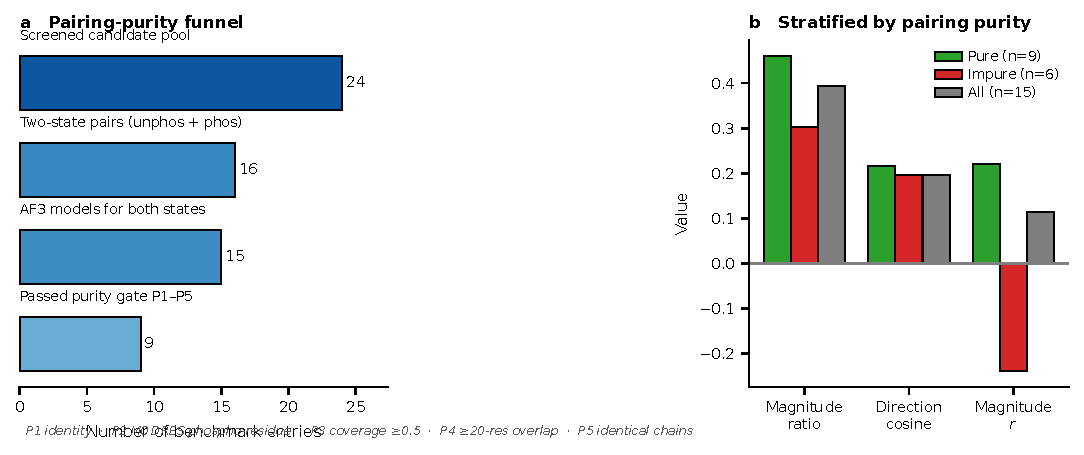
\includegraphics[width=\textwidth]{Fig1_purity_funnel.pdf}
\caption{\textbf{Pairing purity shapes the benchmark and the conclusion.}
(a) Funnel from the screened candidate pool through the two-state and
AF3-availability filters to the pairs passing the P1--P5 purity gate.
(b) The same frozen per-protein results stratified by pairing purity,
showing the median amplitude ratio, median direction cosine and magnitude
correlation for pure ($n=9$), impure ($n=6$) and all ($n=15$) pairs.
Purity here means chain-composition matching (P5), not ligand matching: the
nine pure pairs are not identical apart from the phosphate, and two of them
carry engineered substitutions (AURKA T287D, one residue from the site;
PAK1 K299R, present in both states); a further pair outside the pure
stratum (IKBKB) uses an S177E/S181E phosphomimetic non-phospho reference.
See Sec.~\ref{sec:purity} and the confound audit shipped with the data.}
\label{fig:funnel}
\end{figure*}

\begin{figure*}[t]
\centering
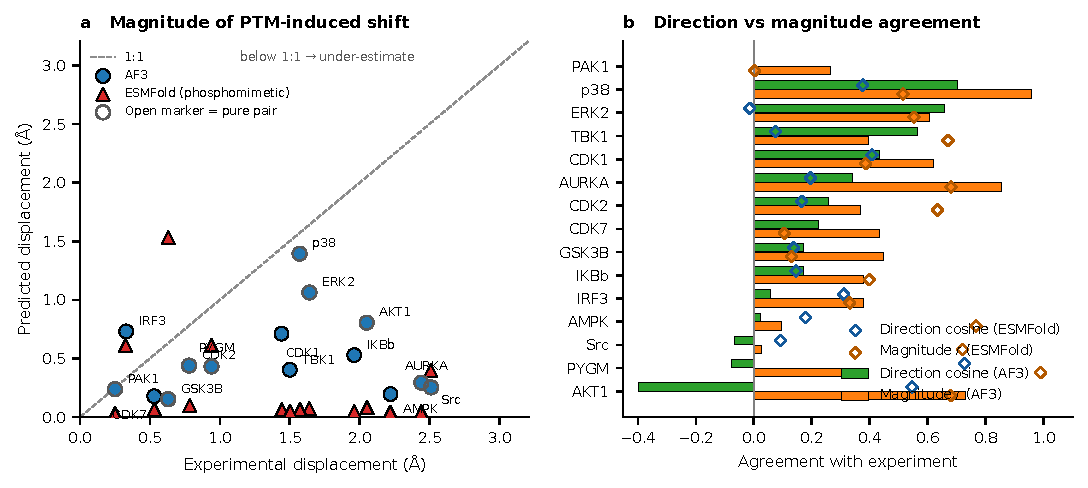
\includegraphics[width=\textwidth]{Fig2_af3_vs_pdb.pdf}
\caption{\textbf{Predicted versus experimental phosphorylation-induced
displacement.} (a) Per-protein mean experimental displacement against the
predicted displacement for AF3 (circles) and ESMFold with a phosphomimetic
phospho state (triangles); the dashed line is $1{:}1$. Open markers denote
purely paired structures. (b) Per-protein direction cosine and magnitude
correlation for AF3 (bars) and ESMFold (diamonds). Neither predictor's
displacement tracks the experimental one.}
\label{fig:fig2}
\end{figure*}

\begin{figure*}[t]
\centering
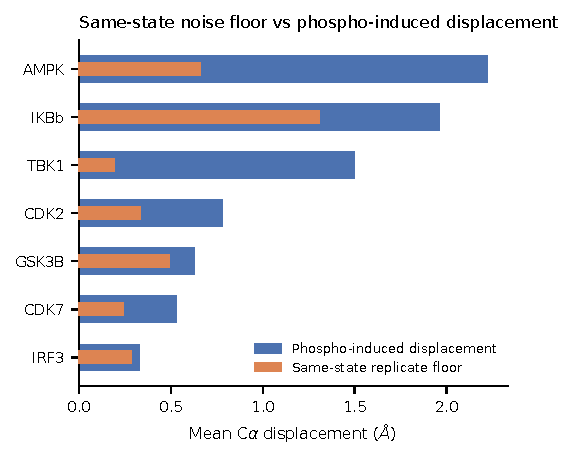
\includegraphics[width=\textwidth]{FigS1_noise_floor.pdf}
\caption{\textbf{Same-state noise floor.} Experimental same-state
dispersion (crystallographically independent copies) and predictor
same-state dispersion (across AF3 models) compared with the
phosphorylation-induced experimental displacement.}
\label{fig:noise}
\end{figure*}

\begin{figure*}[t]
\centering
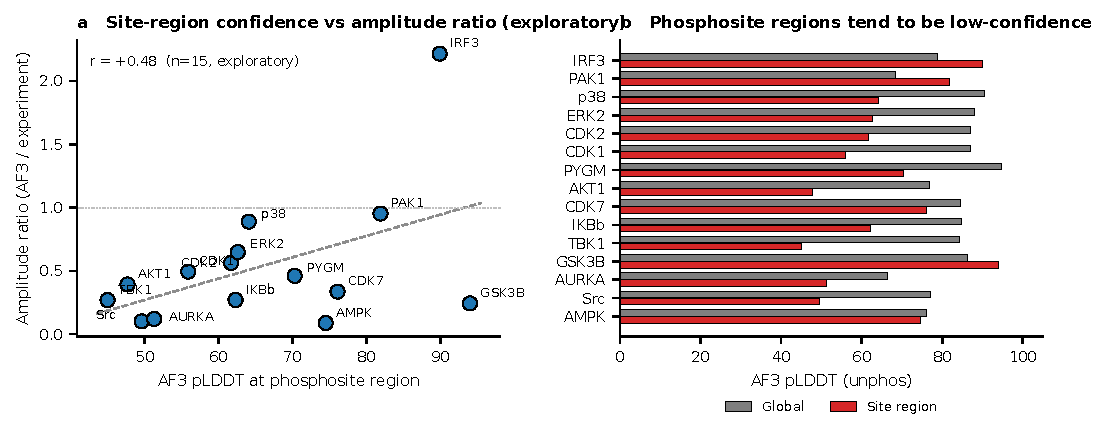
\includegraphics[width=\textwidth]{Fig4_plddt_vs_amplitude.pdf}
\caption{\textbf{Site pLDDT and agreement.} (a) Site-region pLDDT against
amplitude ratio for the 15 pairs (labelled), with a least-squares fit; the
apparent association is carried by IRF3 and collapses when it is removed
(Sec.~\ref{sec:res-confidence}). (b) Site-region versus global pLDDT,
showing that phosphosite regions tend to be lower-confidence than the rest
of the chain.}
\label{fig:plddt}
\end{figure*}

\begin{figure*}[t]
\centering
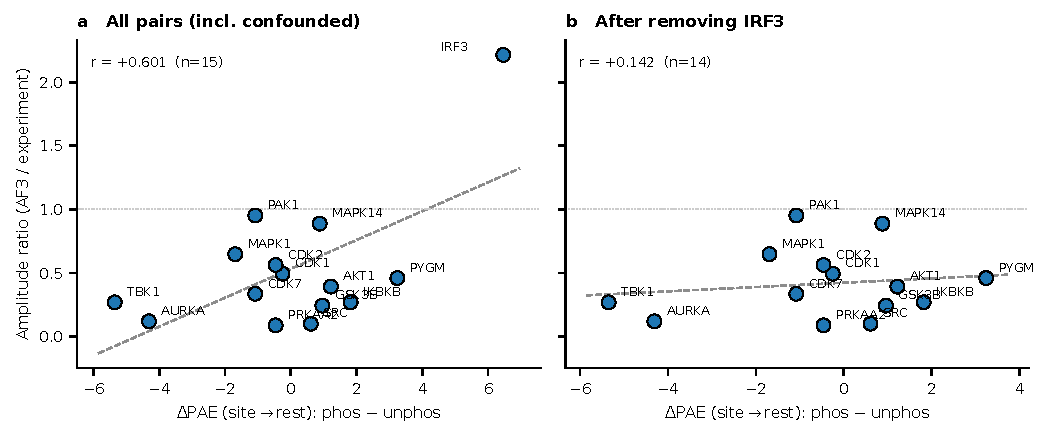
\includegraphics[width=\textwidth]{Fig5_pae_leverage.pdf}
\caption{\textbf{$\Delta$PAE association is a single-point effect.}
$\Delta$PAE (site$\rightarrow$rest) against amplitude ratio, all pairs
(left) and after removing IRF3 (right).}
\label{fig:pae}
\end{figure*}

\begin{figure*}[t]
\centering
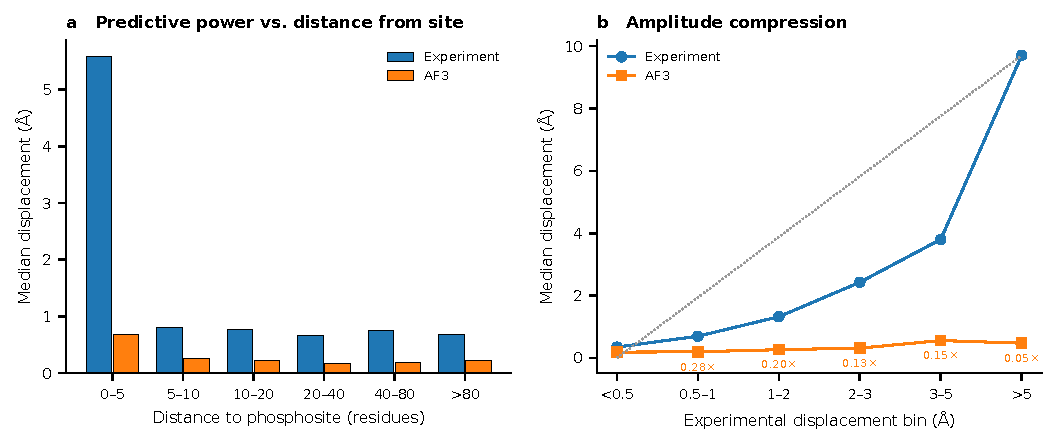
\includegraphics[width=\textwidth]{Fig3_residue_spectrum.pdf}
\caption{\textbf{Residue-level response saturates.} Median
predicted/experimental displacement ratio as a function of experimental
displacement magnitude, over all 5{,}148 common residues across the 15
cohort proteins; the decline is monotone across the six bins. The analysis
uses the first AF3 model of each state (model 0), not a multi-model average.
A distance decomposition of the same residues shows no trend
(Sec.~\ref{sec:res-explore}).}
\label{fig:spectrum}
\end{figure*}

\end{document}
